 % arara: clean: { files: [thesis.aux, thesis.bbl, thesis.blg, thesis.dvi, thesis.fdb_latexmk, thesis.fls, thesis.idx, thesis.ilg, thesis.ind, thesis.lof, thesis.log, thesis.lot, thesis.nlo, thesis.nls, thesis.out, thesis.pdf, thesis.ps, thesis.toc]}
% arara: latex:  { shell: yes }
% arara: bibtex
% arara: nomencl
% arara: latex
% arara: makeindex
% arara: latex:  { shell: yes }
% arara: dvips
% arara: ps2pdf

% ******************************* PhD Thesis Template **************************
% Please have a look at the README.md file for info on how to use the template

\documentclass[a4paper,12pt,times,numbered,print,index,custombib]{Classes/PhDThesisPSnPDF}

% ******************************************************************************
% ******************************* Class Options ********************************
% *********************** See README for more details **************************
% ******************************************************************************

% `a4paper'(The University of Cambridge PhD thesis guidelines recommends a page
% size a4 - default option) or `a5paper': A5 Paper size is also allowed as per
% the Cambridge University Engineering Deparment guidelines for PhD thesis
%
% `11pt' or `12pt'(default): Font Size 10pt is NOT recommended by the University
% guidelines
%
% `oneside' or `twoside'(default): Printing double side (twoside) or single
% side.
%
% `print': Use `print' for print version with appropriate margins and page
% layout. Leaving the options field blank will activate Online version.
%
% `index': For index at the end of the thesis
%
% `draft': For draft mode without loading any images (same as draft in book)
%
% `draftmode': Special draft mode with line numbers, images, and water mark with
% timestamp and custom text. Position of the text can also be modified.
%
% `abstract': To generate only the title page and abstract page with
% dissertation title and name, to submit to the Student Registry
%
% `chapter`: This option enables only the specified chapter and it's references
%  Useful for review and corrections.
%
% ************************* Custom Page Margins ********************************
%
% `custommargin`: Use `custommargin' in options to activate custom page margins,
% which can be defined in the preamble.tex. Custom margin will override
% print/online margin setup.
%
% *********************** Choosing the Fonts in Class Options ******************
%
% `times' : Times font with math support. (The Cambridge University guidelines
% recommend using times)
%
% `fourier': Utopia Font with Fourier Math font (Font has to be installed)
%            It's a free font.
%
% `customfont': Use `customfont' option in the document class and load the
% package in the preamble.tex
%
% default or leave empty: `Latin Modern' font will be loaded.
%
% ********************** Choosing the Bibliography style ***********************
%
% `authoryear': For author-year citation eg., Krishna (2013)
%
% `numbered': (Default Option) For numbered and sorted citation e.g., [1,5,2]
%
% `custombib': Define your own bibliography style in the `preamble.tex' file.
%              `\RequirePackage[square, sort, numbers, authoryear]{natbib}'.
%              This can be also used to load biblatex instead of natbib
%              (See Preamble)
%
% **************************** Choosing the Page Style *************************
%
% `default (leave empty)': For Page Numbers in Header (Left Even, Right Odd) and
% Chapter Name in Header (Right Even) and Section Name (Left Odd). Blank Footer.
%
% `PageStyleI': Chapter Name next & Page Number on Even Side (Left Even).
% Section Name & Page Number in Header on Odd Side (Right Odd). Footer is empty.
%
% `PageStyleII': Chapter Name on Even Side (Left Even) in Header. Section Number
% and Section Name in Header on Odd Side (Right Odd). Page numbering in footer


% ********************************** Preamble **********************************
% Preamble: Contains packages and user-defined commands and settings
% ******************************************************************************
% ****************************** Custom Margin *********************************

% Add `custommargin' in the document class options to use this section
% Set {innerside margin / outerside margin / topmargin / bottom margin}  and
% other page dimensions
\ifsetCustomMargin
  \RequirePackage[left=37mm,right=30mm,top=35mm,bottom=30mm]{geometry}
  \setFancyHdr % To apply fancy header after geometry package is loaded
\fi

% *****************************************************************************
% ******************* Fonts (like different typewriter fonts etc.)*************

% Add `customfont' in the document class option to use this section

\ifsetCustomFont
  % Set your custom font here and use `customfont' in options. Leave empty to
  % load computer modern font (default LaTeX font).
  \RequirePackage{helvet}
\fi

% *****************************************************************************
% **************************** Custom Packages ********************************

% ************************* Algorithms and Pseudocode **************************

%\usepackage{algpseudocode}


% ********************Captions and Hyperreferencing / URL **********************

% Captions: This makes captions of figures use a boldfaced small font.
%\RequirePackage[small,bf]{caption}

\RequirePackage[labelsep=space,tableposition=top]{caption}
\renewcommand{\figurename}{Fig.} %to support older versions of captions.sty


% *************************** Graphics and figures *****************************

%\usepackage{rotating}
%\usepackage{wrapfig}

% Uncomment the following two lines to force Latex to place the figure.
% Use [H] when including graphics. Note 'H' instead of 'h'
%\usepackage{float}
%\restylefloat{figure}

% Subcaption package is also available in the sty folder you can use that by
% uncommenting the following line
% This is for people stuck with older versions of texlive
%\usepackage{sty/caption/subcaption}
\usepackage{subcaption}

% ********************************** Tables ************************************
\usepackage{booktabs} % For professional looking tables
\usepackage{multirow}

%\usepackage{multicol}
%\usepackage{longtable}
%\usepackage{tabularx}


% ***************************** Math and SI Units ******************************

\usepackage{amsfonts}
\usepackage{amsmath}
\usepackage{amssymb}
\usepackage{siunitx} % use this package module for SI units


% ******************************* Line Spacing *********************************

% Choose linespacing as appropriate. Default is one-half line spacing as per the
% University guidelines

% \doublespacing
% \onehalfspacing
% \singlespacing


% ************************ Formatting / Footnote *******************************

% Don't break enumeration (etc.) across pages in an ugly manner (default 10000)
%\clubpenalty=500
%\widowpenalty=500

%\usepackage[perpage]{footmisc} %Range of footnote options


% *****************************************************************************
% *************************** Bibliography  and References ********************

%\usepackage{cleveref} %Referencing without need to explicitly state fig /table

% Add `custombib' in the document class option to use this section
\ifuseCustomBib
   \RequirePackage[square, sort, numbers, authoryear]{natbib} % CustomBib

% If you would like to use biblatex for your reference management, as opposed to the default `natbibpackage` pass the option `custombib` in the document class. Comment out the previous line to make sure you don't load the natbib package. Uncomment the following lines and specify the location of references.bib file

%\RequirePackage[backend=biber, style=numeric-comp, citestyle=numeric, sorting=nty, natbib=true]{biblatex}
%\bibliography{References/references} %Location of references.bib only for biblatex

\fi

% changes the default name `Bibliography` -> `References'
\renewcommand{\bibname}{References}


% *****************************************************************************
% *************** Changing the Visual Style of Chapter Headings ***************
% This section on visual style is from https://github.com/cambridge/thesis

% Uncomment the section below. Requires titlesec package.

%\RequirePackage{titlesec}
%\newcommand{\PreContentTitleFormat}{\titleformat{\chapter}[display]{\scshape\Large}
%{\Large\filleft{\chaptertitlename} \Huge\thechapter}
%{1ex}{}
%[\vspace{1ex}\titlerule]}
%\newcommand{\ContentTitleFormat}{\titleformat{\chapter}[display]{\scshape\huge}
%{\Large\filleft{\chaptertitlename} \Huge\thechapter}{1ex}
%{\titlerule\vspace{1ex}\filright}
%[\vspace{1ex}\titlerule]}
%\newcommand{\PostContentTitleFormat}{\PreContentTitleFormat}
%\PreContentTitleFormat


% ******************************************************************************
% ************************* User Defined Commands ******************************
% ******************************************************************************

% *********** To change the name of Table of Contents / LOF and LOT ************

%\renewcommand{\contentsname}{My Table of Contents}
%\renewcommand{\listfigurename}{My List of Figures}
%\renewcommand{\listtablename}{My List of Tables}


% ********************** TOC depth and numbering depth *************************

\setcounter{secnumdepth}{2}
\setcounter{tocdepth}{2}


% ******************************* Nomenclature *********************************

% To change the name of the Nomenclature section, uncomment the following line

%\renewcommand{\nomname}{Symbols}


% ********************************* Appendix ***********************************

% The default value of both \appendixtocname and \appendixpagename is `Appendices'. These names can all be changed via:

%\renewcommand{\appendixtocname}{List of appendices}
%\renewcommand{\appendixname}{Appndx}

% ******************************** Draft Mode **********************************

% Uncomment to disable figures in `draftmode'
%\setkeys{Gin}{draft=true}  % set draft to false to enable figures in `draft'

% These options are active only during the draft mode
% Default text is "Draft"
%\SetDraftText{DRAFT}

% Default Watermark location is top. Location (top/bottom)
%\SetDraftWMPosition{bottom}

% Draft Version - default is v1.0
%\SetDraftVersion{v1.1}

% Draft Text grayscale value (should be between 0-black and 1-white)
% Default value is 0.75
%\SetDraftGrayScale{0.8}


%% Todo notes functionality
%% Uncomment the following lines to have todonotes.

%\ifsetDraft
%	\usepackage[colorinlistoftodos]{todonotes}
%	\newcommand{\mynote}[1]{\todo[author=kks32,size=\small,inline,color=green!40]{#1}}
%\else
%	\newcommand{\mynote}[1]{}
%	\newcommand{\listoftodos}{}
%\fi

% Example todo: \mynote{Hey! I have a note}

\usepackage{tabularx}

% ************************ Thesis Information & Meta-data **********************
% Thesis title and author information, refernce file for biblatex
% ************************ Thesis Information & Meta-data **********************
%% The title of the thesis
\title{Routers Reconfigurables de Altas Prestaciones}
%\texorpdfstring is used for PDF metadata. Usage:
%\texorpdfstring{LaTeX_Version}{PDF Version (non-latex)} eg.,
%\texorpdfstring{$sigma$}{sigma}

%% Subtitle (Optional)
\subtitle{Proyecto de Grado}

%% The full name of the author
%\author{Autores: \\Emiliano Viotti\\Rodrigo Amaro}

\author{ \fontsize{11pt}{12pt}\selectfont Autores: \\ {\normalfont Emiliano Viotti \\ Rodrigo Amaro } \\ \vspace{1cm} Supervisores: \\ {\normalfont Dr. Eduardo Grampin \\ MSc. Martin Giachino}}

%% Department (eg. Department of Engineering, Maths, Physics)
\dept{\fontsize{12pt}{12pt}\selectfont Instituto de Computación}

%% University and Crest
%\university{Universidad de la República}
\crest{
	
\includegraphics[width=0.185\textwidth]{Udelar} 
	\hspace{3cm}
	
\includegraphics[width=0.25\textwidth]{fing}
	\vspace{1cm}
}

%% You can redefine the submission text:
% Default as per the University guidelines:
% ``This dissertation is submitted for the degree of''
\renewcommand{\submissiontext}{}

%% Full title of the Degree
%\degreetitle{Proyecto de Grado}

%% College affiliation (optional)
\college{\fontsize{11pt}{12pt}\selectfont Facultad de Ingeniería, Universidad de la República}

%% Submission date
% Default is set as {\monthname[\the\month]\space\the\year}
\degreedate{\fontsize{11pt}{12pt}\selectfont Julio de 2015 \\Montevideo, Uruguay} 

%% Meta information
\subject{LaTeX} \keywords{{LaTeX} {PhD Thesis} {Engineering} {University of
Cambridge}}


% ***************************** Abstract Separate ******************************
% To printout only the titlepage and the abstract with the PhD title and the
% author name for submission to the Student Registry, use the `abstract' option in
% the document class.

\ifdefineAbstract
 \pagestyle{empty}
 %\includeonly{Declaration/declaration, Abstract/abstract}
 %\includeonly{Abstract/abstract}
\fi

% ***************************** Chapter Mode ***********************************
% The chapter mode allows user to only print particular chapters with references
% Title, Contents, Frontmatter are disabled by default
% Useful option to review a particular chapter or to send it to supervisior.
% To use choose `chapter' option in the document class

\ifdefineChapter
 \includeonly{Chapter1/chapter1}
\fi

% ******************************** Front Matter ********************************
\begin{document}

\frontmatter

\begin{titlepage}
  \maketitle
\end{titlepage}


%% ******************************* Thesis Dedidcation ********************************

\begin{dedication} 

Emiliano quiere dedicar \\ 
este trabajo a \\
su hermano Andr\'es, \\
compa\~nero de aventuras \\
y a sus abuelos. 

\vspace{1cm}

Rodrigo quiere dedicar \\ 
este trabajo a \\
su amor Sof\'ia,\\ 
a su padre Jorge\\ 
y su madre Silvia. 


\end{dedication}


%% ******************************* Thesis Declaration ***************************

\begin{declaration}

I hereby declare that except where specific reference is made to the work of 
others, the contents of this dissertation are original and have not been 
submitted in whole or in part for consideration for any other degree or 
qualification in this, or any other university. This dissertation is my own 
work and contains nothing which is the outcome of work done in collaboration 
with others, except as specified in the text and Acknowledgements. This 
dissertation contains fewer than 65,000 words including appendices, 
bibliography, footnotes, tables and equations and has fewer than 150 figures.

% Author and date will be inserted automatically from thesis.tex \author \degreedate

\end{declaration}


%% ************************** Thesis Acknowledgements **************************

\begin{acknowledgements}      
A todos aquellos que estuvieron presentes en los buenos momentos y en especial en los malos, sean familiares, amigos o compa\~neros de carrera. Agradecemos a todos los integrantes del MuDi por el apoyo incondicional en el día a día. A nuestros trabajos y novias que nos comprendieron en momentos de ausencia y nunca cesaron en su apoyo. Adem\'as agradecemos a nuestros tutores, Eduardo y Martin por el permanente apoyo a lo largo de este proyecto, por la ayuda brindada en los momentos m\'as difíciles, a todo el gruopo de investigaci\'on MINA por prestarnos una oficina en la cual trabajar, a la Agencia de Investigaci\'on e Innovaci\'on (ANII) y al proyecto Frida por el apoyo económico brindado.


\end{acknowledgements}

%% ************************** Thesis Abstract *****************************
% Use `abstract' as an option in the document class to print only the titlepage and the abstract.
\begin{abstract}


Actualmente, desarrollar aplicaciones de control de red,  manipular el contenido de un paquete e incluso algo tan simple como analizar un cabezal de un paquete es una tarea difícil que requiere de trabajar a un nivel muy bajo y con un nivel de conocimiento bastante específico, trabajando con herramientas no propietarias y de c\'odigo abierto. Por otro lado si se quiere hacer esto en un contexto comercial con tecnologías propietarias, solo es posible si el equipo o API de funcionalidades disponible así lo permite. Este escenario no hace otra cosa que entorpecer y ralentizar el desarrollo de nuevos protocolos y servicios, así como la innovación en el área. El modelo de las Redes Definidas por Software (SDN) desacopla los planos de control y datos a la vez que estandariza la forma en que cualquier equipo de red puede ser manipulado y así también el tráfico que estos procesan. De esta forma se generan las condiciones para que cualquier equipo pueda ser utilizado de forma transparente en la definición de nuevos servicios y protocolos, independientemente del fabricante facilitando así la innovación en el área. 

En este proyecto se construye un prototipo de red de backbone MPLS utilizando el enfoque SDN y placas de red aceleradas en hardware reconfigurable (NetFPGA), orientado a la provisión de redes privadas virtuales como servicio de cara a lo que podría ser una posible implementación de la nueva red académica RAU2. Se diseña e implementa un equipo enrutador de red denominado RAU-Switch, compatible con las tecnologías IP, MPLS y OpenFlow, orientado a convivir con equipos legados, y a un bajo costo económico. Ademas se desarrolla un conjunto de aplicaciones de control y gestión de red denominado RAUFlow y se contribuye a la comunidad en el desarrollo de documentación exhaustiva en relación a tecnologías muy recientes de las que algunas poco se conoce y otras aun están en fases experimentales.

\textbf{Palabras clave:} Redes de Computadoras, SDN, OpenFlow, NetFPGA, MPLS, Open vSwitch.
\end{abstract}





% *********************** Adding TOC and List of Figures ***********************

\tableofcontents

\listoffigures

\listoftables

% \printnomencl[space] space can be set as 2em between symbol and description
%\printnomencl[3em]

\printnomencl

% ******************************** Main Matter *********************************
\mainmatter

%*******************************************************************************
%****************************** Second Chapter *********************************
%*******************************************************************************

\chapter{Introducci\'on}

\ifpdf
    \graphicspath{{Chapter1/Figs/Raster/}{Chapter1/Figs/PDF/}{Chapter2/Figs/}}
\else
    \graphicspath{{Chapter1/Figs/Vector/}{Chapter1/Figs/}}
\fi


\section{Motivación}

En la actualidad, sobre la red Internet conviven aplicaciones académicas, comerciales y particulares con iguales prioridades. Este escenario no es apropiado para actividades de experimentación, investigación y estudio de nuevas herramientas a gran escala. A su vez los proveedores de servicios sobre Internet, contando con que no todos sus clientes hacen uso de su infraestructura a la vez, venden m\'as servicios de los que realmente puede soportar, lo que hace que no sea viable garantizar un ancho de banda para cada servicio. Esta situación es comúnmente conocida como “sobreventa” del ancho de banda y se agrava en horas de mayor uso de Internet (horas pico), lo cual es crítico cuando se piensa en aplicaciones que requieren de niveles de \gloss{cdeser} garantizados. Por estas razones Internet no parece apropiada para su utilización en el contexto académico, ya que se necesita una red que permita proveer de conectividad y a su vez soportar actividades experimentales como desplegar nuevos servicios y protocolos, así como asegurar determinados parámetros de calidad de servicio.

En este contexto y en todo el mundo se vienen desarrollando desde mediados de la década de los 90’s las redes académicas avanzadas de alta velocidad, con el objetivo de proveer una red que posibilite a docentes e investigadores colaborar en aplicaciones altamente demandantes de ancho de banda   
 (educación a distancia, transferencia de grandes cantidades de información, acceso a equipos remotos, telemedicina, etc.), sin competir por este recurso con aplicaciones de naturaleza comercial. En Estados Unidos por ejemplo, el proyecto que lidera este desarrollo es Internet2\citep{Internet2}, en Canadá es el proyecto CA*net4\citep{Canarie2}, en Europa el proyectos GÉANT\citep{GEANT} y en Asia el proyecto APAN\citep{APAN}. Todas estas redes se encuentran a su vez conectadas entre sí, formando una gran red avanzada de alta velocidad de alcance mundial. En Latinoamérica, las redes académicas de Argentina, Brasil y Chile se encuentran integradas a Internet2.

En las \'ultimas dos d\'ecadas no solo se han hecho esfuerzos para desarrollar las redes académicas nacionales, sino que también se ha trabajado arduamente en la construcción de acuerdos que permitan interconectar cada una de estas redes en una gran red académica de alcance global. Una de las iniciativas que encaus\'o estos esfuerzos fue la denominada CAESAR (Connecting All European and South (Latin) American Researchers), reconociendo la necesidad de crear una red troncal regional en América Latina que eventualmente se pueda conectar a GÉANT y tras la cual se llega a la conocida “Declaración de Toledo”. Poco tiempo después las redes latinoamericanas se unen bajo su propia agrupación denominada CLARA (Cooperación Latino Americana de Redes Avanzadas) y adscriben a dicha declaración\footnote{Datos históricos extraídos de sitio oficial de Red Clara \cite{RedClara}.}.

En Uruguay, la Universidad de la República a través del Servicio Central de Informática (SeCIU), es la fundadora de la Red Académica Uruguaya (RAU). Este proyecto persigue en el contexto de las redes académicas mundiales los siguientes objetivos: unir las Instituciones Nacionales Académicas, Universidades (pública y privadas) y Centros de Investigación del Uruguay, promover el desarrollo de Redes Académicas y Científicas donde ellas hagan falta, planificar y desarrollar una red nacional, incentivar la colaboración con iniciativas similares y conectar la RAU con Latinoamérica. 

La RAU brinda servicios a instituciones educativas y de investigación, as\'i como implementa servicios de la propia Universidad de la República a trav\'es de una red de alcance nacional. Actualmente entre facultades, escuelas, institutos y servicios de la Universidad de la República, así como diversas instituciones educativas y de investigación, son 31 las instituciones que forman parte de la RAU, las cuales hacen uso de los 64 nodos que la conforman para brindar servicios a un total aproximado de 8.000 docentes, 4.000 técnicos y 100.000 estudiantes en diferentes partes del país\footnote{Datos de escala de la RAU aproximados brindados por t\'ecnicos del SeCIU.}.

Por otro lado, se viene trabajando en un proyecto para reemplazar la infraestructura actual de la RAU por una red avanzada de altas prestaciones, que pueda brindar mayores y mejores servicios a las instituciones que forman parte de la misma, así como conectarse a las demás redes académicas de Latinoam\'erica. Este proyecto se denomin\'o RAU2  

\section{Definición del Problema}

El problema elegido como eje para el desarrollo de este trabajo es la construcción de lo que se dio en llamar RAU2, la cual estaría dotada de funciones de virtualización de redes que permitan una gran flexibilidad en su definición y uso. Como red universitaria pretende no solo mejorar el ancho de banda disponible para desarrollar las tareas comunes con cualquier otra red de esta magnitud, sino que además busca virtualizar la red como mecanismo de asignar recursos independientes a cada una de las instituciones que hacen uso de la misma (por ejemplo universidades y centros de investigación) y poder utilizarla al mismo tiempo como laboratorio de pruebas sin que esto interfiera con el funcionamiento normal de la red.

Interesa entonces trabajar en el desarrollo de un prototipo para la RAU2 utilizando como plataforma PCs con placas de red aceleradas en hardware reconfigurable, fruto de un desarrollo de la Universidad de Stanford denominado NetFPGA (Field Programmable Gate Arrays)\citep{NetFPGA} y el enfoque de las Redes Definidas por Software (\gloss{SDN})\citep{gude2008nox}\citep{SDNReadingList}.

\section{Objetivos}
El objetivo principal de este trabajo es la implementación de un prototipo de red de altas prestaciones para la RAU2, utilizando como punto de partida el enfoque de SDN y el hardware NetFPGA, para luego ejecutar un conjunto de pruebas que permitan validar estas tecnologías para su utilización en  la posible construcción de la RAU2.

A su vez dado la ausencia de experiencias similares trabajando con estas tecnologías a nivel local y en la órbita de la academia, se busca conocer a fondo estas tecnologías, en particular la arquitectura de SDN y los lenguajes de programación relacionados, así como generar conocimiento y experiencias que puedan contribuir en trabajos a futuro. Por ello se hizo especial hincapié en la generación de  material sobre el estado del arte de las redes definidas por software y una detallada documentación de la experiencia obtenida utilizando el hardware NetFPGA.

\section{Resultados Esperados}
Los resultados esperados de este proyecto son:

\begin{enumerate}
\item El estado del arte en el enfoque de las Redes Definidas por Software (SDN) y el hardware reconfigurable NetFPGA. En particular interesa conocer en profundidad ambas tecnologías, relevando el nivel de madurez y desarrollo de ellas y reunir suficiente información para evaluar su utilización en la construcción de un prototipo m\'as complejo en funcionalidades y superior en rendimiento.
%que sea equiparable en prestaciones y rendimiento a un producto comercial sustituto.

\item Una implementaci\'on de un prototipo de gesti\'on y control de red utilizando estrategias de SDN, en particular enfocado en las funcionalidades y capacidades que se pretenden de la RAU2.

\item Diseño e implementación de pruebas funcionales que permitan validar el prototipo desarrollado y evaluar el potencial de las tecnologías utilizadas.

\end{enumerate}

\section{Estructura del documento}

A continuación se describe la forma en que est\'a estructurado este documento y las temáticas asociadas a cada cap\'itulo.

El cap\'itulo 2 presenta los resultados obtenidos en la investigación del estado del arte en SDN, NetFPGA y conceptos esenciales para el entendimiento de este trabajo; no es estrictamente necesaria la lectura de las secciones \ref{section2.1},\ref{section2.5} y \ref{section2.6}. Luego en el cap\'itulo 3 se presenta el análisis del problema, en donde se incluyen las principales ventajas en la utilización del enfoque SDN y hardware NetFPGA. En el cap\'itulo 4 se muestra el diseño general del prototipo planteado, mientras que en el cap\'itulo 5 se presenta el diseño de RAUFlow, la aplicaci\'on que implementa el plano de control SDN. Se incluyen en este cap\'itulo los casos de uso implementados en RAUFlow, el modelo de datos diseñado y detalles de la arquitectura e implementaci\'on. En cuanto al cap\'itulo 6, en el se presenta el laboratorio de pruebas diseñado para validar funcionalmente el prototipo junto con los resultados obtenidos. Le sigue el cap\'itulo 7 en donde se ofrece una evaluación de los resultados m\'as importantes, así como un breve estudio de la ejecuci\'on del proyecto. Finalmente en el cap\'itulo 8 se presentan las conclusiones obtenidas a partir del desarrollo de este trabajo y las principales l\'ineas de trabajo e investigaci\'on identificadas como trabajo a futuro.

Adicionalmente se incorpora el cap\'itulo de referencias con la informaci\'on bibliográfica del material utilizado en el desarrollo de este trabajo y un cap\'itulo de ap\'endices. Tambi\'en se anexa un manual para la construcci\'on del dispositivo que se dio a llamar RAU-Switch, orientado a la reproducci\'on y posible mejora a futuro del trabajo realizado.
%*******************************************************************************
%*********************************** First Chapter *****************************
%*******************************************************************************

\chapter{Estado del Arte}  %Title of the Second Chapter

\ifpdf
    \graphicspath{{Chapter2/Figs/Raster/}{Chapter2/Figs/PDF/}{Chapter2/Figs/}}
\else
    \graphicspath{{Chapter2/Figs/Vector/}{Chapter2/Figs/}}
\fi

En este capítulo se presentan los resultados obtenidos en el trabajo de investigación sobre el estado
del arte de las Redes Definidas por Software (Software Defined Networking), lenguajes
de programación y herramientas para el desarrollo sobre dicha arquitectura, hardware NetFPGA y otros conceptos esenciales para el desarrollo de este trabajo. En caso de que el lector desee profundizar en alguno de los conceptos presentados en este cap\'itulo o consultar enfoques alternativos
y/o complementarios se recomiendan los siguientes trabajos~\citep{StateOfArt1}~\citep{StateOfArt2}. Para el caso particular en que el lector este familiarizándose con el enfoque de las Redes Definidas por Software, se sugiere también la lectura de \citep{SDNReadingList} y el libro\citep{SDNBook1}.\\

En relación a como se estructura este cap\'itulo, primero se introduce el concepto de Software Defined Networking (SDN) analizando sus principales antecedentes y finalmente brindando una definición. Luego se presenta y analiza en profundidad una de las arquitecturas existentes basadas en este enfoque y en particular utilizada por este trabajo para la construcción del prototipo. Se contin\'ua con la introducción de algunos conceptos esenciales para el desarrollo de este trabajo como el concepto de Redes Privadas Virtuales y Multilabel Protocol Switch (\gloss{MPLS}) entre otros. Finalmente se presenta el relevamiento en el estado del arte realizado sobre la plataforma NetFPGA.  

%********************************** %First Section  **************************************
\section{Antecedentes de SDN} %Section - 1.1
Software Defined Networking, Redes Definidas por Software en español o simplemente SDN por su sigla en ingl\'es, es un concepto relativamente nuevo ya que bajo este nombre puede contextualizarse en la \'ultima década. No obstante muchas de las ideas que yacen detrás de este enfoque han sido introducidas por diferentes propuestas en el pasado. Por ello vale la pena repasar los principales antecedentes que desde nuestra perspectiva contribuyeron al enfoque de SDN. 

\subsection{Open Signaling}
En el año 1995 el grupo de investigación OPENSIG\cite{campbell1999open} dentro del \gloss{IETF}, comenzó a trabajar en alternativas para hacer ATM, Internet y las redes móviles ``más'' abiertas, extensibles y programables.

El principal objetivo de este grupo fue proveer de un acceso al hardware de red (\gloss{router}s, \gloss{switch}es, etc) mediante un conjunto de interfaces abiertas. Con esto se buscaba permitir el despliegue de nuevos servicios de red a través de un ambiente de programación distribuido.

El principal desafío con el que tuvo que lidiar esta iniciativa fue la estricta arquitectura en forma vertical que presenta el hardware de red (modelo de capas OSI), cuya naturaleza a su vez solía ser cerrada. Esto dificultaba una estricta separación entre el software de control y el hardware.\\

Los esfuerzos de esta iniciativa desembocaron en la especificación del General Switch Managment Protocol (GSMP); un protocolo de propósito general para control de etiquetas en switches.
GSMP permitía a un controlador establecer y liberar conexiones en un dispositivo conmutador de tramas (mejor conocido como switch), agregar, eliminar y dejar una conexión multicast, manejar los puertos de un switch, obtener información acerca de la configuración, obtener y eliminar recursos reservados en un switch y obtener información estadística.\\

Tras años de trabajo, el grupo considero concluido su labor, siendo su último trabajo publicado la especificación de GSMPv3 en Junio del 2002\cite{doria2002general}.

\subsection{Active Networking}
Active Networking\citep{tennenhouse1997survey}\citep{tennenhouse2002towards}\citep{moore2001towards} \'o Redes Activas en español es otra iniciativa que surge en la década de los 90's con la propuesta de una red programable que posibilitara la configuración de servicios sobre la misma. Fue propulsada por la USA Defense Advanced Research Projects Agency (DARPA), con el principal objetivo de acelerar la innovación en una área de redes marcada por la lentitud en incorporar nuevas tecnologías y servicios.\\

Se propusieron dos enfoques: (1) enfoque de Switches Programables en donde el tr\'afico es encaminado a través de nodos que ejecutan programas y cada paquete o su segmento correspondiente es derivado al programa apropiado en el nodo y (2) enfoque de C\'apsulas en donde cada paquete enviado en la red transporta un programa, evaluándose en cada nodo en su ambiente de ejecución correspondiente.\\

Como tal, este proyecto no alcanz\'o la suficiente masa cr\'itica como para imponerse en la industria, entre otras razones por la necesidad de un hardware diferente m\'as caro (tradicionalmente se utilizaba hardware de tipo \gloss{ASIC} y se requería de tipo \gloss{TCAM}, \gloss{FPGA} \'o \gloss{NPU}) adem\'as de interrogantes de seguridad y desarrollo de lenguajes de programación apropiados.

\subsection{Routing Control Platform}
Routing Control Platform (RCP)\citep{feamster2004case}\citep{caesar2005design} o Plataforma de Control de Ruteo, propone una entidad de control (Routing Control Platform) encargada de computar las rutas en una red, que luego utilizando protocolos estándares como iBGP traslada dicha configuración a los diferentes dispositivos.\\ 

Esta estrategia ten\'ia como ventajas que al utilizar protocolos existentes estándares facilitaba notablemente la transición entre el paradigma actual y el propuesto. No obstante su potencial 
se encontraba limitado justamente a las capacidades de los protocolos de comunicación existentes.

\subsection{ForCES Protocol}
Otro grupo de trabajo dentro del IETF denominado ForCES (Forwarding and Control Element Separation) comenzó a trabajar a mediados del año 2007 en un protocolo que permita la separación entre los dispositivos de red y la inteligencia que los gobierna. Dicho protocolo fue especificado como una propuesta de estándar y publicado en el año 2010 bajo el nombre ForCES Protocol\citep{doria2010forwarding}.

Este enfoque plantea dos entidades lógicas denominadas Elementos de Control (CE) y Elementos de Reenv\'io (FE), así como un protocolo de comunicación entre ambas entidades.

\subsection{4D Project}
En el año 2004 el proyecto 4D \citep{rexford2004network}\citep{greenberg2005clean} propone una re-estructuración arquitectónica de una red basada en tres principios claves: 

\begin{itemize}
\item Políticas de red (network-level objectives): conjunto de objetivos o requerimientos sobre una red tales como performance, confiabilidad entre otras.

\item Vistas de la red (network-wide views): vistas globales sobre la topolog\'ia de red, tr\'afico y eventos, con ciertos niveles de frescura y exactitud en los datos.

\item Control directo: se debe proveer de una interfaz directa para el control de los dispositivos de red
\end{itemize}

Basándose en estos principios se construye el esquema denominado ``4D'' que merece su nombre por los cuatro planos presentes en su arquitectura: decisión (decision), diseminación (dissemination), descubrimiento (discovery) y datos (data).\\

Dicha arquitectura hace un fuerte énfasis en una completa separación de lo que son las decisiones lógicas que toma un Sistema Autónomo (\gloss{AS}), del conjunto de protocolos que gobiernan las redes e interacciones entre sus diferentes componentes.\\

Los objetivos al nivel de un AS son especificados en el plano de decisiones y mediante los servicios de los planos de diseminación y descubrimiento se ejerce un control directo sobre como se encamina y redirigen paquetes en el plano de datos.\\

\begin{figure}[htbp!] 
\centering    
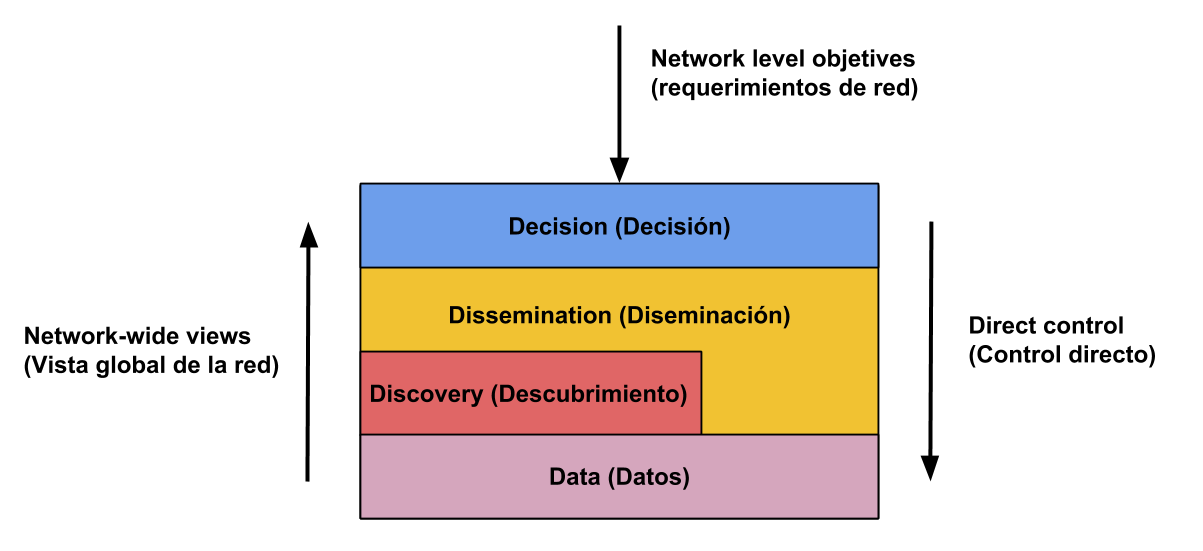
\includegraphics[width=0.8\textwidth]{4DProject3}
\caption[Capas de la arquitectura]{Capas de la arquitectura, imagen extraída de \cite{greenberg2005clean}}
\label{fig:4DProject}
\end{figure}

%En otras palabras el plano de decisión es responsable de crear la configuración de la red, mientras que el plano de diseminación se encarga de recolectar información sobre el estado de la red para el plano de decisión y distribuir la salida del plano de decisión. 

En resumen, utilizando el plano de diseminación se recolecta diferente información acerca del estado de la red, sobre la cual luego el plano de decisión construye las \textit{Políticas de red}. También a través del plano de diseminación se distribuyen dichas políticas a los distintos dispositivos de red. Mientras tanto el plano de descubrimiento permite a dispositivos descubrir vecinos directamente conectados en la red. Finalmente el plano de datos se encarga de redirigir el tráfico de red.\\ \\

Una vez introducidos a los principales antecedentes de las redes definidas por software, en la siguiente secci\'on se propone profundizar en dicho concepto.

\section{Software Defined Networking}
\label{section2.2}

Definir el concepto de Software Defined Networking no es una tarea simple, puesto que no existe una definici\'on \'unica entre las distintas organizaciones que se encuentran trabajando en la temática. En particular se pueden destacar el grupo de trabajo Software-Defined Networking Research Group (SDNRG) del \gloss{IRTF}, quien se encuentra trabajando en la redacción de las definiciones y estándares para este concepto, y la organización Open Networking Foundation (ONF)\cite{ONF} que concentra gran cantidad de material y documentación sobre SDN y adem\'as se encuentra trabajando en el desarrollo del protocolo \gloss{OpenFlow} el cual se explica mas adelante en este trabajo.\\

Acorde a la Open Networking Foundation, SDN puede resumirse como:

\begin{quote}
\textit{``La separación física del plano de control de la red del plano de datos, y donde el plano de control controla varios dispositivos.''}
\end{quote}

Más en detalle, SDN es una arquitectura de red que desacopla los planos de control y de datos, moviendo el plano de control (inteligencia, construcción y c\'alculo de políticas de red) hacia una entidad denominada Controlador. Esto habilita al control de la red a ser directamente programable y a la infraestructura subyacente ser abstraída por las aplicaciones y servicios de red.\\ 

La ONF presenta a SDN como una arquitectura emergente, dinámica, escalable, rentable y adaptable, haciéndola ideal para aplicaciones de naturaleza dinámica y exigentes de los recursos de red disponibles. En particular destaca las cualidades de presentar una gestión centralizada y de estar basada en estándares abiertos neutrales a los vendedores.\\

\begin{figure}[htbp!] 
\centering    
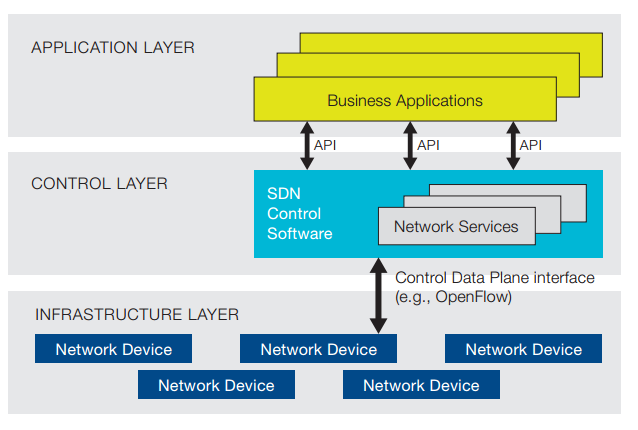
\includegraphics[width=10cm]{SDNArchitecture}
\caption[Arquitectura de SDN - Capas lógicas]{Arquitectura de SDN - Capas lógicas. Imagen extraída de \cite{ONF}}
\label{fig:SDNArchitecture}
\end{figure}

El enfoque de SDN propone tres capas lógicas (ver imagen ~\ref{fig:SDNArchitecture}): (1) capa de aplicaciones (Application Layer), (2) capa de control (Control Layer) y (3) capa de infraestructura  
 (Infraestructure Layer).\\

La capa de infraestructura se compone por los dispositivos de red tradicionales como switches y routers, en particular compatibles con la arquitectura SDN. La inteligencia de dichos dispositivos a diferencia de switches y routers convencionales es retirada de los mismos para ser trasladada a la capa de control.

Cada dispositivo implementa un conjunto de operaciones bien definidas mediante la cual es manipulado por la capa de control. Esta API de operaciones forma parte de lo que se denomina Interfaz Sur.
\\

En la capa de control se encuentra el software encargado de implementar el plano de control en dicho modelo, usualmente denominado Controlador.\\

El Controlador expone un conjunto de operaciones a las aplicaciones SDN de la capa superior(capa de Aplicación) para la manipulación de los dispositivos de la capa inferior (capa de Infraestructura).  Esta API de operaciones es conocida en el modelo bajo el nombre de Interfaz Norte.\\

La capa de aplicaciones, contiene implementado en software (aplicaciones SDN) toda la inteligencia que originalmente se agregaba en un dispositivo de la capa de infraestructura, por ejemplo la implementaci\'on de protocolos de red. En dicha capa se pueden implementar desde protocolos de ruteo como OSPF y \gloss{RIP}, backbones sobre MPLS, políticas de seguridad y hasta aplicaciones de ingeniería de tráfico.

Notese aqu\'i la diferencia entra la capa de aplicaci\'on del modelo de capas OSI y la capa de aplicaci\'on  del modelo SDN. En el modelo SDN, una aplicaci\'on puede implementar protocolos y servicios de cualquier capa del modelo OSI.\\

De esta forma Software Defined Networking centraliza el control de la red en una aplicación de software  
 (Controlador) y transforma algoritmos, procesos de control, políticas de seguridad y toda la inteligencia antiguamente acoplados a los dispositivos de red, en aplicaciones de controlador.\\

\section{Arquitecturas basadas en SDN}
\label{section2.3}

Existen varias arquitecturas o implementaciones en las que de una forma u otra puede encontrarse argumentos para afirmar que siguen el enfoque de SDN. Si bien este trabajo se basa en la utilización de la arquitectura OpenFlow, existen otras arquitecturas basadas en este enfoque como el protocolo ForCES y alternativas m\'as comerciales como OpFlex.

A continuaci\'on se explican los principales conceptos relacionados a la arquitectura OpenFlow.

\subsection{OpenFlow}

Orientado por el enfoque en tres capas de SDN y bajo la misma premisa de desacoplar completamente los planos de datos y control, OpenFlow\cite{mckeown2008openflow} brinda una implementaci\'on estándar para el mecanismo de comunicación entre las capas de control e infraestructura (Interfaz Sur). En otras palabras, provee de un protocolo de comunicación estándar para manipular los distintos dispositivos de la red y así el plano de datos.\\ 

OpenFlow se basa en tres componentes (ver figura ~\ref{fig:OpenFlowArch}): (1) Controlador OpenFlow compatible, (2) Protocolo OpenFlow y (3) Switch OpenFlow compatible.

  
%OpenFlow logra estandarizar la forma mediante la cual cada entrada de la tabla de flujos en un switch, puede ser modificada externamente (Protocolo OpenFlow), brindando un mecanismo transparente y confiable para la manipulación del plano de datos en los switches compatibles con OpenFlow independientemente del vendedor y fabricante del equipo.\\

%Un switch OpenFlow, como se ilustra en la Figura 6, esta compuesto al menos por 3 partes: (1) Una Tabla de Flujos (Flow Table), con una acción asociada a cada flujo en la misma(Flow table entry) para decirle al switch como procesar cada flujo, (2) un Canal Seguro (Secure Channel) que conecta el switch con un proceso de control remoto (Controlador) permitiendo enviar comandos y paquetes entre el controlador y el switch utilizando (3) el protocolo OpenFlow el cual provee una forma abierta y estándar de comunicación entre el controlador y el switch.\\

\begin{figure}[htbp!] 
\centering    
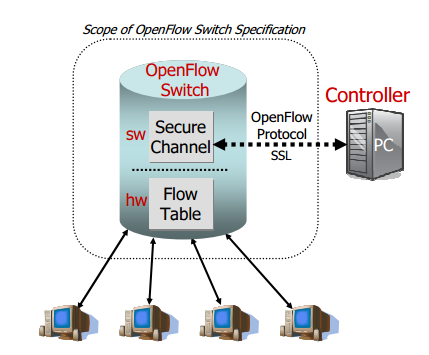
\includegraphics[width=7cm]{OpenFlowArchitecture1}
\caption[Estructura de un switch OpenFlow]{Estructura de un switch OpenFlow. Imagen extraída de \cite{mckeown2008openflow}}
\label{fig:OpenFlowArch}
\end{figure}

Desde la perspectiva de un Controlador OpenFlow, todos los dispositivos de red son equivalentes en sus funcionalidades y se denominan simplemente switches OpenFlow. Un switch OpenFlow se compone de tres componentes principales (ver figura ~\ref{fig:OpenFlowArch}): (1) Tabla de flujos, (2) Canal Seguro 
 (Secure Channel) que conecta el switch con el Controlador habilitando el intercambio de paquetes y comandos entre estos últimos dos utilizando (3) el protocolo OpenFlow.\\
 
Cada switch OpenFlow presenta una o m\'as tablas de flujos. Cada una de las entradas de estas tablas es denominada flujo y determina c\'omo una clase de paquetes deben ser procesados y reenviados.\\

Cada entrada o flujo en esta tabla (ver figura ~\ref{fig:OpenFlowArch2}) se compone de: (1) campos de selección (matching fields), utilizados para identificar a un conjunto de paquetes a ser tratados de una forma en particular, basándose en información relacionada a campos en los cabezales del paquete para esto; (2) contadores para la recolección de información estadística en relación al flujo (n\'umero de paquetes recibidos, cantidad de bytes, duración de un flujo, etc.) y (3) un conjunto de instrucciones y acciones que son aplicadas a cada paquete que coincide con el flujo descrito. Estos campos establecen la forma en que un paquete es procesado y reenviado.
 
\begin{figure}[htbp!] 
\centering    
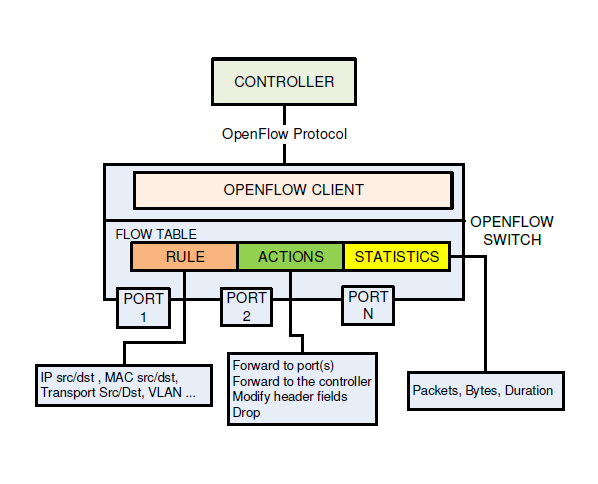
\includegraphics[width=9cm]{OpenFlowArchitecture2}
\caption[Visión esquemática del funcionamiento de un Switch OpenFlow]{Visión esquemática del funcionamiento de un Switch OpenFlow. Imagen extraída de \cite{mckeown2008openflow}}
\label{fig:OpenFlowArch2}
\end{figure}

Cuando un paquete arriba a un switch (ver figura ~\ref{fig:OFPacketProcessing}), se extraen y comparan cabezales del paquete acorde a las reglas definidas en el matching field del flujo, comparando los campos utilizados. En caso que el paquete coincida con las reglas definidas, se aplican el conjunto de instrucciones y acciones asociadas a dicho flujo. En caso que el paquete no coincida con ningún flujo, el accionar a desempeñar dependerá del conjunto de instrucciones y acciones definidas por una entrada especial en la tabla de flujos, denominada Table-miss Flow Entry.\\ 

\begin{figure}[htbp!] 
\centering    
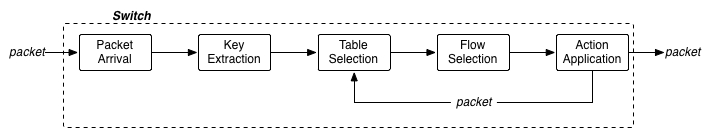
\includegraphics[width=12cm]{OFPacketProcessing}
\caption[Ciclo de vida de un paquete en pipe OpenFlow]{Ciclo de vida de un paquete en el pipe OpenFlow}
\label{fig:OFPacketProcessing}
\end{figure}


La Table-miss Flow Entry esta pensada para contemplar el tr\'afico que no es definido por ningún otro flujo, por ello en esencia es el ultimo flujo a ser considerado (menor prioridad) al momento de procesar un paquete. Generalmente tiene asociada la acción de eliminar el paquete (Drop), procesar el paquete en la siguiente tabla de flujos (GoTo Table) \'o reenviar el paquete al Controlador.\\

Otra caracter\'istica importante de un switch OpenFlow, es la capacidad para procesar paquetes utilizando protocolos tradicionales de red adem\'as del procesamiento normal de OpenFlow. Esta característica a su vez da lugar a la clasificaci\'on en switches OpenFlow puros y switches OpenFlow h\'ibridos. Mientras que los switches OpenFlow puros son aquellos que solamente soportan el protocolo de igual nombre, los switches OpenFlow h\'ibridos son aquellos que adicionalmente permiten procesar paquetes de la misma forma en que lo har\'ia un hardware de red legado.

Aprovechando las capacidades de un switch OpenFlow h\'ibrido, se puede definir por ejemplo la Table-Flow-Entry de forma que se procese todo paquete contemplado por esta entrada como un hardware de red tradicional, aplicando por ejemplo esquemas de reenvío IP. 

\subsection{Reglas OpenFlow}
Cada entrada en la tabla de flujos, distingue un tipo de tr\'afico en particular y la forma en que se procesa (acciones e instrucciones). Es uno de los pilares del protocolo la expresividad disponible para escribir las reglas de cada flujo; es decir, la capacidad de agrupar tipos de tr\'afico acorde a diferentes propiedades en el mismo.\\

\begin{figure}[h] 
\centering    
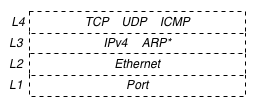
\includegraphics[width=6cm]{ofv1MF}
\caption[OF 1.0 Matching Fields]{OpenFlow v1.0 Matching Fields}
\label{fig:OF10MatchingFields}
\end{figure}

Las reglas OpenFlow se basan en los valores de cabezales asociados a diferentes capas del modelo OSI. Estos cabezales a su vez varían con la versi\'on del protocolo, incorporándose m\'as opciones en cada versi\'on del mismo. Por ejemplo en la versi\'on 1.0 del protocolo se tiene un soporte mínimo para cabezales de capas 1 a 4 (ver imagen ~\ref{fig:OF10MatchingFields}).

Por otro lado en la version 1.3.3 del protocolo se cuenta soporte para utilizar cabezales de IPv6, ICMPv6 y MPLS en la definición de los flujos (ver imagen ~\ref{fig:OF13MatchingFields}).
 
\begin{figure}[ht] 
\centering    
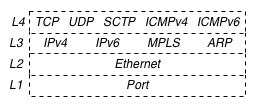
\includegraphics[width=6cm]{ofv13MF}
\caption[OF 1.3.3 Matching Fields]{OF 1.3.3 Matching Fields}
\label{fig:OF13MatchingFields}
\end{figure}

\subsection{Acciones OpenFlow}

Como se menciona anteriormente la acci\'on de un flujo OpenFlow determina la forma en que un paquete es procesado en un switch. Las tres acciones principales que todo switch OpenFlow debe implementar son:

\begin{enumerate}
\item \textbf{[Output:Puerto]:} Reenviar un paquete hacia un puerto determinado (o conjunto de puertos). Esto permite encaminar paquetes a través de la red.

\item \textbf{[Output:Controller]:} Encapsular y reenviar un paquete hacia el Controlador. Utilizando el canal de comunicación con el Controlador y el protocolo OpenFlow, se reenvía el paquete al plano de Control. Esto permite procesar un paquete no identificado en ningún flujo en cualquier momento o en una etapa de configuración de la red. Luego el Controlador decide si descartar el paquete o instalar un nuevo flujo que lo contemple.

\item \textbf{[Drop]:} Descartar un paquete. Puede ser utilizado por razones de seguridad, para prevenir ataques de negación de servicios (\gloss{DoS}), eliminar paquetes sospechosos, disminuir el impacto de paquetes de descubrimiento en redes de difusión (broadcast), o simplemente descartar paquetes no contemplados.
\end{enumerate}

\subsection{Controlador OpenFlow}
Un controlador SDN brinda implementaciones a las Interfaces Sur y Norte. Un controlador OpenFlow/SDN requiere adem\'as de esto la compatibilidad con el protocolo OpenFlow en la interfaz sur. 

Basándose solamente en estos principios, las implementaciones de controladores OpenFlow pueden ser muy variadas. Desde controladores muy simples como NOX\cite{ControllersNOX} y POX\cite{ControllersPOX} que siguen estrictamente el enfoque de SDN/OpenFlow, hasta controladores m\'as elaborados como OpenDaylight\cite{ControllersOpendaylight} (ver imagen ~\ref{fig:OpenDayLightHydrogen}) que implementan OpenFlow como una característica mas de su implementaci\'on de interfaz Sur.

Sin embargo existen aspectos relacionados a la entidad Controlador dentro del enfoque SDN/OpenFlow que son afines a cualquier implementaci\'on y arquitectura. A continuaci\'on se mencionan los principales:
  
\begin{figure}[ht!] 
\centering    
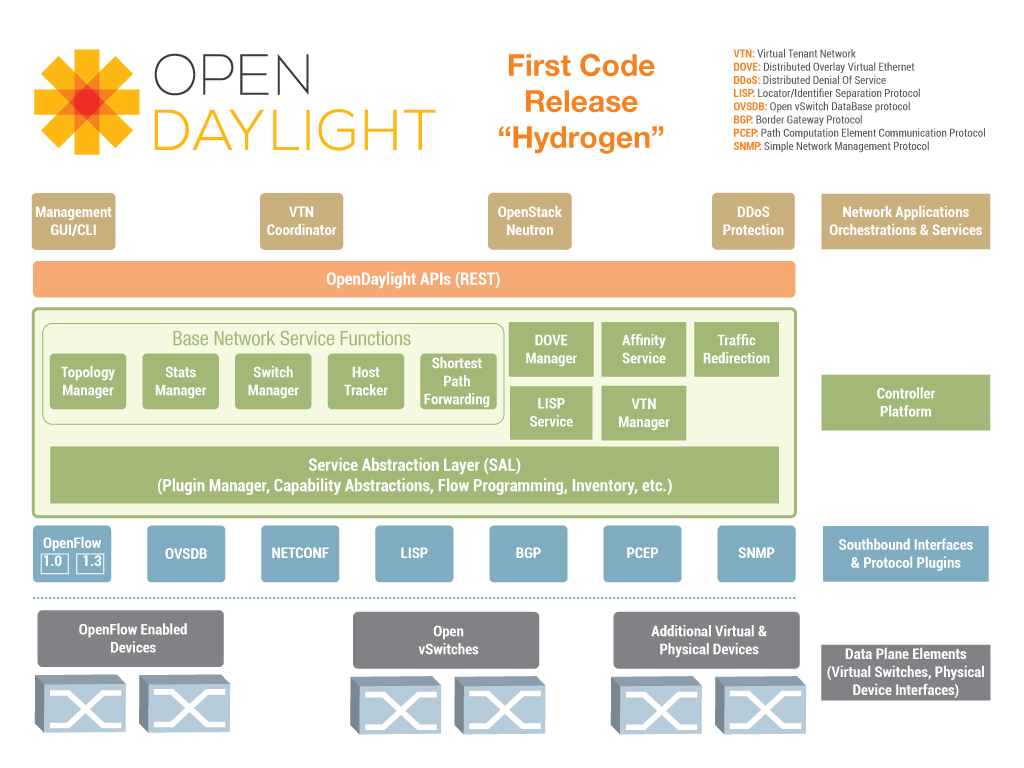
\includegraphics[width=1\textwidth]{opendaylight-hydrogen}
\caption[Arquitectura de OpenDaylight Hydrogen]{Arquitectura de OpenDaylight Hydrogen. Imagen extraída de \cite{OpenDaylightArch}}
\label{fig:OpenDayLightHydrogen}
\end{figure}

\subsubsection{Granularidad en el control}
Tradicionalmente, la unidad básica de tráfico en una red es el paquete. Cada paquete contiene información de direccionamiento necesaria para la toma de decisiones dentro del switch a nivel de reenvío. Sin embargo muchas aplicaciones de red envían datos como un flujo de muchos paquetes individuales, mientras que las redes que desean proveer de calidad de servicios (\gloss{QoS}) se benefician utilizando flujos. Por ello resulta beneficioso adoptar un nivel de abstracción superior en el control del plano de datos, distinguiendo tr\'afico por flujos y a través de paquetes individuales.\\
 
Por otro lado uno de los puntos vulnerables del enfoque SDN, es la comunicación entre switch y Controlador. Sobrecargar este canal de comunicación, pensando en redes a gran escala en la cantidad de dispositivos, supone una debilidad importante. Basar la granularidad de control en paquetes individuales, profundiza esta debilidad; mientras que el enfoque basado en flujos atenúa esta debilidad. 

Para fijar ideas, en el enfoque de flujos, cuando un paquete recibido no es contemplado por ning\'un flujo particular puede ser reenviado al Controlador para decidir su procesamiento. \'Este tras analizar dicho paquete puede resolver adem\'as del procesamiento instalar un nuevo flujo para contemplar m\'as adelante paquetes similares (incluyendo al mismo paquete). De esta forma cualquier otro paquete contemplado por el nuevo flujo no es m\'as reenviado al Controlador, mientras que en el enfoque de paquetes individuales la regla instalada contemplar\'ia solamente al paquete inicial.

A su vez se pueden utilizar las mismas prácticas que con el control a nivel
de paquetes individuales, como agrupar flujos relacionados al tráfico entre dos hosts, tomando
decisiones sobre los flujos agregados. 

\subsubsection{Centralizado vs Distribuido}
SDN no establece ninguna restricción en cuanto a si el plano de control debe ser tanto lógica como físicamente centralizado o distribuido. De hecho resulta conveniente pensar en enfoques distribuidos cuando se piensa en arquitecturas robustas y escalables. No es el objetivo de este trabajo profundizar en esta área de investigación por lo cual se recomienda para profundizar sobre esta temática las referencias \cite{heller2012controller} y \cite{levin2012logically}. 

En relación a OpenFlow, si bien el protocolo no establece mecanismos para la comunicación entre controladores, habilita a un switch a conectarse a múltiples controladores.\\

Algunos proyectos como Onix\cite{koponen2014distributed} e HyperFlow\cite{tootoonchian2010hyperflow} toman la idea de mantener un plano de control lógicamente centralizado, pero físicamente distribuido. Este enfoque tiene como principal beneficio disminuir la sobrecarga en el proceso de búsqueda sobre una tabla de flujos, permitiendo la comunicación con controladores locales.\\

Kandoo\cite{hassas2012kandoo}, proponen utilizar controladores locales para el manejo de aplicaciones y redirigir hacia un Controlador global flujos que requieran de una visión global del estado de la red, bastante similar a lo anterior. Esto tiene como principal beneficio la reducción de la carga sobre el Controlador global, debido al filtrado de solicitudes de flujo que realizan los controladores locales, y a la vez proveen al plano de datos de una rápida respuesta para las solicitudes que pueden ser manejadas por los controladores locales.\\

Concluyendo con este apartado, otro de los enfoques que buscan generar una distribución del plano de control en SDN es el asumido por FlowVisor\cite{sherwood2010carving}. Este enfoque propone la virtualización de una red de switches OpenFlow con múltiples controladores, construyendo lo que denominan Slices de la red. De esta forma brindan a cada controlador una visión local a su slice; mientras que un controlador especial actuá de \gloss{Proxy}, manteniendo una visión global de toda la red.

\subsubsection{Políticas reactivas vs proactivas}
Existen dos enfoques para la intervención del controlador en el plano de datos: (1) reactivo y (2) proactivo.

\begin{enumerate}
\item \textbf{Instalación reactiva de políticas:} En este enfoque, un switch se configura con la tabla de flujos vac\'ia o al menos una configuración mínima al encenderse. Luego, cada vez que un paquete arriba al switch y no es contemplado por ning\'un flujo, es reenviado al Controlador. Este decide que hacer con el paquete e instala un flujo en el dispositivo para procesar de igual forma paquetes similares.

Este modelo adoptado en particular por Ethane\cite{casado2007ethane}, presenta como principal desventaja la sobrecarga en el canal de comunicación Switch-Controlador. Por ello juega un rol sumamente importante en este esquema la definición de los flujos (flujos m\'as generales disminuyen la sobrecarga con el controlador y flujos muy específicos aumentan esta sobrecarga), tiempo de vida de los flujos en la tabla (flujos con tiempo de vida de un solo paquete aumentan la sobrecarga), la ubicación física del controlador y las características del canal de comunicación. Utilizando una jerarquía de controladores, canales de comunicación de alta velocidad o redundancia de enlaces, se puede mejorar la penalizaci\'on en los tiempos de respuesta por la sobrecarga del canal de comunicación. 

\item \textbf{Instalación proactiva de políticas:} En este enfoque, un switch se configura con la mayor cantidad de flujos posibles, contemplando la mayor cantidad de tr\'afico en la red al momento de encender el switch. Luego, cuando un paquete ingresa al switch, en caso de no ser contemplado por ninguno de los flujos instalados, se reenvía al Controlador para decidir c\'omo actuar. Luego el Controlador puede instalar un flujo para contemplar el caso asociado a este paquete. 

En \cite{yu2011scalable} se analiza el impacto de utilizar un enfoque de políticas proactivas en la performance de una red.  

\end{enumerate} 

%\subsubsection{Escalabilidad}
%[No se si aplique hablar de esto capaz es mucho]

\section{Herramientas SDN/OpenFlow disponibles}

La principal herramienta para el desarrollo de aplicaciones SDN/OpenFlow es el software de control o Controlador. No obstante también existen entornos de emulación compatibles con estas tecnologías y que merecen la pena ser mencionados en este trabajo por su utilidad.

\subsection{Controlador}
Existe un cantidad interesante de propuestas para la implementaci\'on del plano de control. En este trabajo se ha mencionado algunos como OpenDaylight, NOX y POX, pero existen varias alternativas. Pueden encontrarse desde controladores comerciales y académicos, en código abierto y propietario, compatibles solamente con OpenFlow y compatibles con múltiples protocolos incluyendo OpenFlow, etc.\\   

Estas características son utilizadas en este proyecto para la elección de la mejor alternativa de software de control, basándose en las necesidades y restricciones del prototipo. Por ello se cree conveniente incluir el siguiente cuadro comparativo, en el que se presentan las principales características utilizadas en la elecci\'on del controlador m\'as apropiado. Cabe destacar que esta tabla esta basada en una tabla m\'as reducida presentada en \cite{StateOfArt1}.\\

\newpage
\clearpage
\begin{table}[htbp!]
\fontsize{7pt}{8pt}\selectfont
\begin{tabular}{|l|l|l|p{2cm}|l|p{5cm}|}
\hline   
\textbf{Controlador} & \textbf{Implementación} & \textbf{Opensource} & \textbf{Desarrollador}         & \textbf{OpenFlow} & \textbf{Detalle}                                                                                                                                                                                                                                                                                                          \\
\hline
POX\cite{ControllersPOX}                  & Python                  & Si                  & Nicira                         & 1.0               & Controlador de propósito general implementado en Python, compatible con Linux, Mac OS, y Windows.                                                                                                                                                                                                                         \\
\hline
NOX\cite{ControllersNOX}                  & C++                     & Si                  & Nicira                         & 1.0               & Uno de los primeros controladores ampliamente utilizado. Implementa funcionalidades para descubrimiento de topologías, learning switch, y Network-wide switch.                                                                                                                    \\
\hline
OpenMUL\cite{ControllersOpenMUL}          & C                       & Si                  & Kulcloud                       & 1.4               & Controlador basado en OpenFlow con compatibilidad hacia atrás (OpenFow v1.0, v1.2, etc) con soporte multi-thread basado en lenguaje C, soporte SSL, soporte a múltiples interfaces norte, API REST                                                                                                                        \\
\hline
Maestro\cite{ControllersMaestro}              & Java                    & Si                  & Rice University                & -                 & Maestro es un controlador orientado a la orquestaci\'on de aplicaciones de control de red. Provee de interfaces para el acceso y modificación de los dispositivos de la red a estas aplicaciones, as\'i como para coordinar la interacci\'on entre ellas. \\
\hline
Trema\cite{ControllersTrema}                & Ruby/C                  & Si                  & NEC                            & 1.0               & Framework full-stack para el desarrollo de Controladores OpenFlow en Ruby y C, compatible con Ubuntu 13.04 y Fedora 16-19 entre otras distribuciones Linux.                                                                                                                                                                \\
\hline
Beacon\cite{ControllersBeacon}           & Java                    & Si                  & Stanford                       & 1.0              & Controlador multi-plataforma, rápido y modular basado en Openflow con soporte a programación orientada a eventos y concurrente (threads). Incorpora la plataforma web Jetty y un modulo GUI extensible.                                                                                                                   \\
\hline
Jaxon\cite{ControllersJaxon}                & Java                    & Si                  & Desarrolladores independientes & 1.0              & Controlador OpenFlow basado en NOX para desarrollo en  Java.                                                                                                                                                                                                                                                              \\
\hline
Helios\cite{ControllersHelios}               & C                       & No                  & NEC                            & -                 & Controlador basado en OpenFlow orientado a lenguaje C, extensible. Interfaz de comunicación Norte en formato Shell.                                                                                                                                                                                                       \\
\hline
Floodlight\cite{ControllersFloodlight}           & Java                    & Si                  & BigSwitch                      & 1.3               & Controlador SDN basado en OpenFlow, soporte para switches virtuales y físicos, maneja redes OpenFlow y redes no OpenFlow así como islas OpenFlow, soporte a OpenStack.                                                                                                                                                     \\
\hline
SNAC\cite{ControllersSNAC}                 & C++                     & No                  & Nicira                         & -                 & Controlador basado en OpenFlow para redes LAN con GUI y un lenguaje definido para declarar reglas. Esta basado en el controlador NOX más un módulo para un lenguaje de modelado formal  
 (FML).                                                                                                                             \\
\hline
\gloss{Ryu}\cite{ControllersRyu}                  & Python                  & Si                  & NTT, OSRG group                & 1.4               & Framework de programación para SDN, provee Controladores basados en OpenFlow, Netconf, Of-config entre otros. Brinda soporte para OpenFlow v1.0 v1.2 v1.3 y v1.4 y extensiones propuestas por le empresa Nicira.                                                                                                                                    \\
\hline
Nodeflow\cite{ControllersNodeFlow}             & Javascript              & Si                  & NTT, OSRG group                &                   & Controlador basado en OpenFlow orientado a programación en Javascript, basado en el framework Node.js.                                                                                                                                                                                                                    \\
\hline
OVS-Controller\cite{OVSController}       & C                       & Si                  & Desarrolladores independientes & -                 & Controlador basado en OpenFlow de referencia con soporte a Open vSwitch y gran parte de otros tipos de switches. Como resultado los switches funcionan como un Switch de capa 2 MAC-learning.                                                                                                                             \\
\hline
FlowVisor\cite{ControllersFlowvisor}            & C                       & Si                  & Stanford/Nicira                & -                 & Controlador de propósitos particulares, que actúa como proxy de forma transparente entre una red OpenFLow y múltiples Controladores OpenFlow.                                                                                                                                                                             \\
\hline
RouteFlow\cite{ControllersRouteflow}            & C++                     & Si                  & CPqD                           & 1.3               & Proyecto opensource que provee de servicios de routing virtualizados sobre hardware OpenFlow. Un escenario de uso común puede ser su utilización en conjunto con otro Controlador como Ryu.                                                                                                                                \\
\hline
OpenDaylight\cite{ControllersOpendaylight}         & Java                   & Si                  & Linux Foundation               & 1.3               & Open Daylight es un framework abierto a la comunidad y apoyado por fabricantes, orientado a mejorar y agilizar la adopción de nuevos protocolos y aplicaciones así como e innovación. Este controlador esta desarrollado en java y provee diferentes m\'odulos de conexión para la interfaz Sur, entre los cuales se encuentra el protocolo OpenFlow. Brinda soporte al protocolo OpenFlow hasta versión 1.3 actualmente.\\
\hline   
\end{tabular}
\caption[Principales controladores disponibles]{Principales controladores disponibles (Basada en una tabla similar y más reducida en \cite{StateOfArt1})}
\label{table:Controladores}
\end{table}

\newpage
\subsection{Mininet y mini NExT}
\textbf{Mininet}\cite{Mininet1} es un emulador de red, que habilita a crear hosts, switches, links y controladores, en un entorno virtual. Se encuentra disponible tanto para instalarse nativamente en un entorno Linux, como a través de una m\'aquina virtual configurada con todo el software de desarrollo necesario para iniciarse en el desarrollo de aplicaciones OpenFlow/SDN (Mininet Kit Starter). 

Soporta diferentes versiones del protocolo OpenFlow y es una de las herramientas m\'as utilizadas para la prototipaci\'on y experimentación de aplicaciones desarrolladas en dicha arquitectura; puesto que habilita a investigadores y desarrolladores, aprender, prototipar, probar y depurar aplicaciones rápidamente utilizando una computadora convencional.\\

\textbf{mini NExT} es una extension de Mininet que permite entre otras cosas asignar a cada host su propio sistema de ficheros, permitiendo as\'i modificar la configuraci\'on por defecto de cada nodo virtual e instalar diferentes herramientas en ellos. Esta orientado al despliegue virtual de arquitecturas m\'as complejas que las posibles con Mininet.\\   

En este trabajo Mininet es utilizado para realizar pruebas de experimentaci\'on y benchmark con las alternativas de controladores disponibles, con el objetivo de determinar el controlador OpenFlow a ser utilizado en la arquitectura del prototipo.\\

\section{Aplicaciones de SDN}
SDN presenta un campo de aplicación bastante extenso, y es posible que a medida que el concepto siga evolucionando y asentándose se irán descubriendo nuevos casos de uso y campos de aplicación. A continuación se muestran algunos casos de uso:

\begin{itemize}

\item \textbf{Monitorizaci\'on de Red:}
En una arquitectura OpenFlow por ejemplo, cada switch provee de información estadística (similar a SNMP) de cada flujo en tiempo real. De esta forma un Controlador puede recolectar información estadística sobre el tráfico en el plano de datos, lo cual es de gran interés para operadores de red y aplicaciones, con la granularidad exacta que estos requieran. Esta información puede ser agregada de diferentes formas: por dirección IP, por dirección MAC, etiquetas VLAN, por aplicación, etc. De esta forma se logra una gran versatilidad en la entrega de información estadística sobre el tráfico en una red.

\item \textbf{Redes \gloss{Tap} programables:}
Utilizando OpenFlow se pueden implementar taps de redes programables en forma centralizada de una forma simple, transparente y eficiente. También pueden filtrarse los datos que son enviados por ejemplo a un sistema de detección de intrusos (IDS), reduciendo la carga de trabajo a los dispositivos de procesamiento de datos utilizados, filtrando previamente los datos que son realmente necesarios y evitando replicar datos innecesarios.\\
Además desde que el control de los dispositivos intermediarios puede realizarse desde un controlador, se facilita enormemente a gestión de los mismos, permitiendo una configuración dinámica en caso de fallas o averías técnicas.

%Utilizando OpenFlow se pueden implementar redes taps
%programables y replicar el tráfico para su monitoreo de una forma más eficiente que los
%métodos tradicionales de SPAN/RSPAN. También pueden filtrarse los datos que son
%enviados por ejemplo a un sistema de detección de intrusos(IDS), reduciendo la carga
%de trabajo a los dispositivos de procesamiento de datos utilizados, filtrando previamente
%los datos que son realmente necesarios y evitando replicar datos innecesarios.
%Además desde que el control de los dispositivos intermediarios puede realizarse desde
%un controlador, se facilita enormemente a gestión de los mismos, permitiendo una
%configuración dinámica en caso de fallas o averías técnicas.

\item \textbf{Balanceo de carga y QoS:}
Contar con una visión global de los dispositivos del plano de datos, habilita al Controlador a implementar diferentes políticas de balanceo de carga en función del estado de la red y permite un uso óptimo de todos los recursos disponibles. A su vez se pueden priorizar diferentes tipos de tráfico, encaminar tráfico dependiendo de un tipo de servicio o contenido y otras técnicas de QoS.

\item \textbf{Herramientas para mitigación de ataques DoS:}
Herramientas para la mitigación de ataques de negación de servicios (DoS) pueden beneficiarse de las estadísticas provistas por un switch OpenFlow por ejemplo para detectar anomalías. Además utilizando la acción de redirección de un flujo al Controlador, se puede analizar y detectar tráfico sospechoso de ataques DoS, permitiendo a posteriori insertar un flujo en el switch de ingreso específico para bloquear el tipo de ataque o tráfico malicioso detectado. 

De todos modos vale la pena recordar la inconveniencia de sobrecargar el canal de comunicaci\'on entre un dispositivo y el controlador. 

\item \textbf{Implementaci\'on de Servicios de red:}
Con una arquitectura basada en SDN como openFlow, resulta sumamente sencillo la incorporación de servicios al plano de datos de una infraestructura de red dada. Independientemente de la marca del hardware utilizado, sus características y funcionalidades, siempre que sean compatibles con OpenFlow puede incorporarse nuevos servicios como autenticación, firewall, almacenamiento secundario, etc., simplemente programando una nueva aplicación en el Controlador que implemente dichos servicios.

\item \textbf{Experimentación:}
El desarrollo, verificación y puesta en producción de nuevos servicios y protocolos resulta sumamente sencillo puesto que consta simplemente de desplegar una nueva aplicación en un entorno de software 
 (Controlador). Por ello resulta sumamente útil el enfoque de SDN para la academia y la industria en lo que refiere al desarrollo de nuevos protocolos de red, nuevos servicios, mejoras a servicios existentes, entre otros.

\end{itemize}

Por estas razones soluciones basadas en el enfoque SDN con OpenFlow por ejemplo, u otras arquitecturas basadas en SDN resultan de gran utilidad en escenarios como:

\begin{enumerate}
\item Redes empresariales
\item Centros de cómputo (Data Centers)
\item Academia
\end{enumerate}

\section{Casos de éxito de SDN}
OpenFlow en particular se ha hecho con un cierto protagonismo recientemente. Tal es el hecho que se pueden nombrar casos de éxito en la migración de servicios sobre esquemas tradicionales de redes a SDN/OpenFlow.\\

La Open Networking Foundation en particular elabor\'o un articulo\cite{ONFSuccessCase} en donde se recomiendan métodos y se proveen guías para la migración de servicios desde un esquema tradicional a SDN, nombrando en particular tres casos de éxito en este tipo de migraciones, en escenarios reales: (1) Google InterDatacenter WAN, (2) NTT Provider Edge y (3) Stanford Campus Network.

Por mayores detalles en relación a estos casos de \'exitos se recomienda continuar con la lectura en dicho articulo.

%A continuaci\'on se explica en detalle el primer caso de éxito, en relaci\'on a los otros dos casos se sugiere continuar la lectura en \cite{ONFSuccessCase}.

%\textbf{Google InterDatacenter:}\\

%Los servicios de Google orientados a usuarios de Internet como su motor de búsquedas, Google+, GMail, Youtube, Google Maps, entre otros, requieren que una gran cantidad de datos sean movidas desde una región a otra todo el tiempo, haciendo a estas aplicaciones y servicios consumidores intensivos de la WAN. Debido a esto Google concluy\'o que la oferta de dichos servicios no sería escalable con las tecnologías disponibles actualmente, debido a la complejidad en la configuración y manejo de dichas tecnologías las cuales no son lineales con el crecimiento en la demanda de dichos servicios. Como resultado, Google decidió apostar por el enfoque de SDN para el manejo de su \gloss{WAN}. Si el lector est\'a interesado en esta experiencia, puede encontrar una descripción completa en \cite{jain2013b4}.

%\item NTT Provider Edge:

%En el modelo de despliegue tradicional de BGP, los routers  proveedores de servicios de borde(Provider Edge Roputer), mantienen numerosas adyacencias BGP; tantas como routers/caminos BGP para diferentes familias de direcciones, como IPv4, IPv6, VPNv4, VPNv6, etc.\\
 
%Mantener la máquina de estados de BGP, procesar las actualizaciones BGP y configuraciones de políticas, calcular los mejores caminos para cada familia de direcciones, constituyen una gran carga de procesamiento en el hardware del router. Adicionalmente los servicios por definición están sujetos a modificaciones en el tiempo, ya sea para proveer de servicios a nuevos clientes como para actualizar sus políticas. Por otro lado los recursos disponibles como CPU y memoria son limitados, y la naturaleza de los sistemas operativos y hardware de cada equipo es propietaria de la implementación de cada fabricante. Esto limita la aceleración de servicios y la innovación a las políticas de cada vendedor de hardware.\\

%Por ello BGP free edge, define un nuevo paradigma que simplifica el encaminamiento eBGP en los routers PE. En este modelo de despliegue, el router PE se convierte en un nodo de reenvío para manejar el plano de datos, mientras que el plano de control BGP se desacopla a una entidad externa. El plano de control de SDN/Openflow encaja perfectamente en el rol de dicha entidad.\\

%Algunas de las razones por las cuales apostar por BGP free edge:
%\begin{itemize}
%\item Simplificar y abaratar la arquitectura de un router PE-BGP con una política BGP centralizada.
%\item Acelerar el despliegue de nuevos servicios de borde mediante la separación en plano de control y %plano de datos
%\item Mejor control sobre patrones de tráfico
%\item Flexibilidad para calcular mejores caminos configurables
%\item Reducción del efecto ``BGP Wave'', ayudando a la escalabilidad de Internet.
%\end{itemize}

%\item Stanford Campus Network:

%Una parte de la red del campus de la Universidad de Stanford, fue exitosamente migrada para soportar %OpenFlow en el año 2010.
%Inicialmente esta migración fue orientada a usuarios en particular (wireless), luego se agregaron los %usuarios físicamente conectados por cable en el ala 3A del edificio William Gates, y finalmente se %expandió en múltiples islas a través de 2 edificios.

%\end{enumerate}

\section{Red Privada Virtual}
\label{section2.7}

En pocas palabras una Red Privada Virtual o VPN por su sigla en ingl\'es, es la extension de una red privada sobre una infraestructura de red p\'ublica como lo es por ejemplo Internet.

Este concepto habilita a un equipo en una determinada subred privada a enviar y recibir información a otro equipo en otra subred separadas f\'isicamente, utilizando una infraestructura de red p\'ublica o compartida para la comunicaci\'on entre ambas subredes, y de la misma forma que si estuviese directamente conectada a la red privada. Adem\'as permite mantener las políticas de seguridad y funcionalidades de la red privada.\\

%Conceptualmente se han propuesto tres arquitecturas b\'asicas de redes VPN: (1) VPN de acceso remoto, (2) VPN punto a punto y (3) VPN sobre LAN.\\

Las implementaciones de redes privadas se caracterizan entre otras cosas por las funcionalidades que son capaces de proveer. En relaci\'on a aspectos de seguridad se buscan principalmente funcionalidades de autenticaci\'on de usuarios, confidencialidad e integridad de los datos. Por otro lado en relaci\'on al procesamiento del tr\'afico dentro de la red p\'ublica, algunas implementaciones de VPN ofrecen funcionalidades de clasificaci\'on de tr\'afico y calidad de servicios (QoS), permitiendo por ejemplo garantizar un ancho de banda m\'inimo para el tr\'afico de una organizaci\'on cuando es transportado a trav\'es de la red p\'ublica de una red privada a otra. 

Algunas implementaciones proveen adem\'as la capacidad de priorizar tipos de tr\'afico como por ejemplo el asociado a una aplicaci\'on en particular, o distribu\'ir la carga entre diferentes caminos, lo que se conoce como balanceo de carga.\\

%Pensando en el contexto de la RAU, alguna de estas funcionalidades como la clasificaci\'on de tr\'afico, priorizaci\'on de tr\'afico por aplicaciones y balanceo de carga se adaptan muy bien a los requerimientos existentes para la nueva versi\'on de la misma(RAU2).\\  

En relaci\'on a la implementaci\'on de redes privadas, a lo largo de los años han surgido diferentes alternativas; diferenciándose por las funcionalidades que implementan y tambi\'en por las capas en el stack OSI en la cual operan. Algunos ejemplos son: 

\begin{itemize}
\item VPN tradicionales
	\begin{itemize}
	\item Frame Relay (Capa 2)	
	\item ATM (Capa 2)
	\end{itemize}
	
\item VPNs basadas en \gloss{CPE}
	\begin{itemize}
	\item L2TP (Capa 2)
	\item IPSec (Capa 2)
	\end{itemize}
	
\item VPNs implementadas por proveedores de servicios
	\begin{itemize}
	\item VPN de capa dos con MPLS (Capa 2)
	\item \gloss{BGP}/MPLS VPNs de capa tres (Capa 3)
	\end{itemize}
\end{itemize}

Otra de las características por la cual es interesante diferenciar a dichas implementaciones, es la capacidad de conectar dos o m\'as puntos de una red privada, lo cual da lugar a redes privadas punto a punto \'o multipunto.

\subsubsection{Redes Privadas Punto a Punto}

Las redes privadas punto a punto son un tipo de implementaci\'on orientada a conectar solamente dos extremos de la red de una organizaci\'on, utilizando lo que se denominan t\'uneles sobre la infraestructura de un proveedor de servicios o Internet. T\'ipicamente se utilizan para conectar un cliente con un servidor en una organizacai\'on cuando se encuentran f\'isicamente separados, o dos edificios de una misma organizaci\'on de una forma simple. 

\begin{figure}[htbp!] 
\centering    
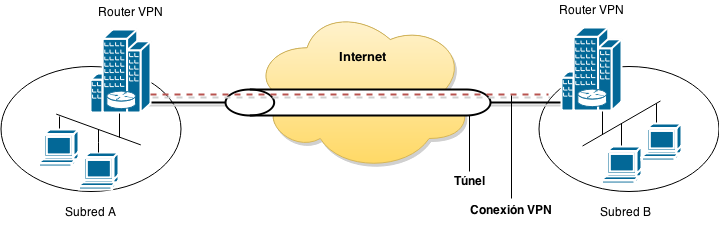
\includegraphics[width=0.7\textwidth]{VPNPuntoaPunto}
\caption[Esquema de una VPN Punto a Punto]{Esquema de una VPN Punto a Punto}
\label{fig:VPNPuntoAPunto}
\end{figure}

En este enfoque el tr\'afico de la subred A al llegar al nodo de borde, es encapsulado y enviado a trav\'es de un túnel sobre la red p\'ublica. Al llegar al otro extremo del túnel el tr\'afico es desencapsulado y entregado al nodo de borde en la subred B, tomando luego el camino correspondiente dentro de esta subred en forma normal. Esto genera la percepci\'on desde ambas subredes que se tiene un “cable” entre ambos nodos de borde, conectando ambas subredes como si fuesen una sola red privada.
 
\subsubsection{Redes Privadas Multipunto}

Las redes privadas multipunto, extienden el enfoque punto a punto con el objetivo de brindar conectividad a una organizaci\'on dispersa geogr\'aficamente en m\'ultiples lugares.

Permiten establecer dominios de difusi\'on compartidos, creando de forma transparente la ilusi\'on de que se tiene una gran LAN compuesta por varias subredes. Sin embargo al ser m\'as completas en funcionalidades y casos de uso soportados, tambi\'en son m\'as complejas de implementar.\\ 

Virtual Private LAN Service (VPLS), es una implementaci\'on de red privada multipunto, bastante difundida y provista de los dos enfoques definidos en los \gloss{RFC}4761\citep{kompella2007virtual} y RFC4762\cite{lasserre2007virtual}. Esta implementaci\'on crea dominios de difusión Ethernet utilizando diferentes tecnologías como IP/MPLS, L2TPv3 y túneles GRE.

\begin{figure}[htbp!] 
\centering    
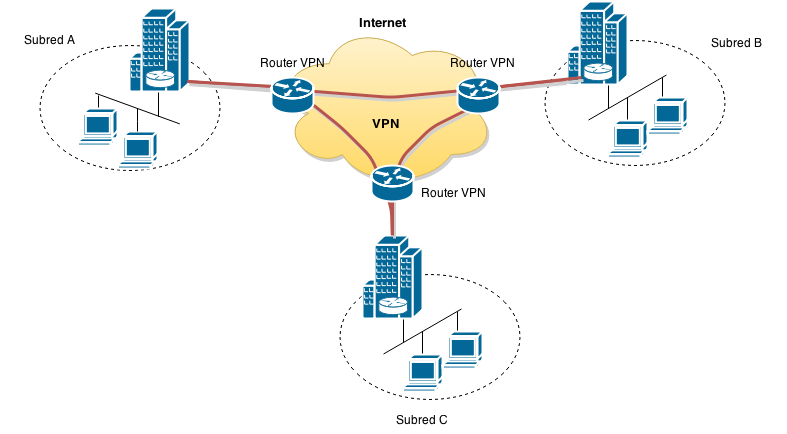
\includegraphics[width=0.7\textwidth]{VPNMultipunto}
\caption[Esquema de una VPN Multipunto]{Esquema de una VPN Multipunto}
\label{fig:VPNMulipunto}
\end{figure}
 
En una red privada multipunto VPLS como la de la figura \ref{fig:VPNMulipunto}, compuesta por las subredes A, B y C, cuando se origina un paquete en un equipo de la subred A con destino a otro equipo en la subred B sucede lo siguiente: (1) primero el paquete es encaminado al nodo de borde de la subred A (Router VPN), (2) luego se resuelve din\'amicamente a que punto de la VPN debe ser enviado el paquete (subred B \'o subred C), para lo cual se utiliza un protocolo de ruteo de borde como BGP, después (3) el paquete es encapsulado dentro de MPLS y encaminado mediante conmutaci\'on de etiquetas hasta el nodo de borde en la subred B, finalmente (4) el paquete es desencapsulado y entregado a la subred B para su encaminamiento normal hacia el equipo destino.

\subsection{Redes Privadas en Uruguay y proyecciones para la RAU}
En Uruguay ANTEL (el principal proveedor de servicios de telecomunicaciones del país) ofrece servicios de redes privadas basados en tres tecnolog\'ias principalmente\footnote{Informaci\'on extraida en base a los servicios comerciales ofrecidos por ANTEL en su sitio oficial \cite{ANTELVPN}}: 

\begin{itemize}
\item Lan to Lan con conexiones Ethernet punto a punto
\item VLAN Hub con conexiones Ethernet 
\item VPN IP/MPLS multipunto con QoS opcionalmente.\\
\end{itemize} 

Dentro de las proyecciones existentes para la RAU2, se encuentran funcionalidades como calidad de servicios, clasificaci\'on de tr\'afico y priorizaci\'on del mismo de acuerdo a pol\'iticas definidas. A su vez se busca conectar m\'ultiples oficinas y organizaciones dispersas geogr\'aficamente en todo el país, manteniendo las pol\'iticas de seguridad de la red privada de cada organizaci\'on. 

De acuerdo a las implementaciones mencionadas anteriormente, la soluci\'on que m\'as se adapta a los requerimientos de la RAU2 es una VPN IP/MPLS multipunto con funcionalidades de QoS, en donde el rol de proveedor de servicios lo asume la propia red académica o la organizaci\'on encargada de su mantenimiento (SeCIU).\\ 

Para complementar la lectura en relaci\'on a la arquitectura de una implementaci\'on de VPN IP/MPLS Multipunto recomendamos continuar con RFC2547\citep{rosen1999bgp} y RFC4364\citep{rosen2006bgp}.

\section{Multiprotocol Label Switching}
\label{section2.8}

Multiprotocol Label Switching (MPLS) o conmutación de etiquetas con soporte para múltiples protocolos, es un mecanismo de transporte de datos desarrollado y estandarizado por el IETF, en particular por los RFC 3031\cite{rosen2001multiprotocol}, 3032\citep{rosen2001mpls} y 3814\citep{nadeau2004multiprotocol}.\\

De acuerdo al modelo de capas OSI, MPLS opera entre las capas de Red y Enlace. Fue diseñado para unificar el servicio de transporte de datos basado en circuitos virtuales y en conmutación de paquetes.\\

MPLS sustituy\'o a los servicios de Frame Relay y ATM en la construcci\'on de servicios de redes privadas, siendo hoy en d\'ia el est\'andard de facto para esto y contando con una amplia adopci\'on de fabricantes.\\

%Actualmente cuenta con una amplia adopción por parte de fabricantes y se ha convertido en el est\'andard de facto  para la construcci\'on de servicios de redes privadas, sustituyendo a los servicios de Frame Relay y ATM.\\
 
MPLS incluye una gran cantidad de características entre las cuales se distinguen soporte para VPNs, Ingeniería de Tráfico, calidad de servicios (QoS), clases de servicios (CoS), a la vez que es independiente del protocolo de capa de enlace pudiendo operar por ejemplo sobre ATM ó Ethernet.\\

En una red MPLS, cuando un paquete ingresa se le coloca un cabezal MPLS. Este cabezal esta compuesto por cuatro campos: Label, Exp, S, TTL. De ellos se destacan el valor de la etiqueta MPLS, utilizada para encaminar paquetes a través de la red hacia su nodo destino, y eventualmente realizar clasificación de tr\'afico.

En cada nodo de la red, el cabezal MPLS es extraído y analizado para determinar el próximo nodo al que se debe enviar dicho paquete. Luego del procesamiento un nuevo cabezal MPLS con otra etiqueta es colocado en el paquete y se reenvía hacia el siguiente nodo en la red.

De esta forma el paquete es encaminado dentro de la red MPLS mediante la conmutaci\'on de etiquetas, hasta que el paquete arriba a un nodo de salida de la red, en donde el paquete ya no contiene etiquetas.\\

Por otro lado, un paquete MPLS puede presentar más de un cabezal MPLS solapados. Esta superposición de etiquetas se conoce bajo el nombre de pila o stack MPLS. De esta forma se pueden agregar más variables al servicio que simplemente encaminar paquetes en la red, como puede ser distinguir entre diferentes tipos de tráfico.\\

Otro punto a destacar de este protocolo es la configuración del plano de reenvío. El plano de control de las redes MPLS se componen de un algoritmo de ruteo y un algoritmo de distribución de etiquetas. Mientras que con el primero se calculan los mejores caminos que un paquete debe tomar para atravesar la red, el segundo se encarga de la asignación y distribución de etiquetas para que cada switch conmute correctamente el paquete hasta su destino.\\

Algunos de los principales términos en la definici\'on del protocolo MPLS son:

\begin{itemize}
\item LER (Label Edge Router): Elemento de la red MPLS por la cual ingresa o egresa tráfico hacia o desde la misma.
\item LSR (Label Switching Router): Elemento de la red MPLS que conmuta etiquetas.
\item FEC (Forwarding Equivalence Class): Nombre asignado al tráfico que es encaminado bajo una misma etiqueta. En otras palabras, es una clase de equivalencia de tráfico a la cual se le asigna una etiqueta.
\item LSP (Label Switched Path): Nombre genérico que se le asigna a un camino MPLS para tráfico de una determinada FEC, es decir un túnel MPLS establecido entre dos extremos de la red.
\item \gloss{LDP} (Label Distribution Protocol): Protocolo de distribución de etiquetas MPLS entre los equipos de la red.
 
\end{itemize}
\vspace{1cm}

%Hasta ahora, se ha presentado un resumen del trabajo de estudio en el estado del arte en las redes definidas por software y se han introducido los principales conceptos para el correcto entendimiento de este trabajo. Resta entonces presentar las conclusiones obtenidas en el trabajo de estudio del estado del arte del hardware NetFPGA. La siguiente secci\'on esta destinada a esta empresa.

En la siguiente secci\'on se presenta un resumen del estudio en el estado del arte realizado sobre la plataforma NetFPGA.

\section{NetFPGA}
\label{section2.9}

NetFPGA\cite{NetFPGA1} es una plataforma de hardware reconfigurable y software de c\'odigo abierto (Open Source), flexible y potente, diseñada para un uso académico en tareas de investigación y enseñanza.\\

El hardware esta basado en un chip FPGA (Field Programmable Gate Array), el cual se programa con lenguajes de descripci\'on de hardware (\gloss{HDL}) como por ejemplo \gloss{VeriLog}. Cuenta con una amplia variedad de proyectos desarrollados tanto por el equipo de NetFPGA (proyectos de referencia), como por instituciones académicas y comerciales involucradas (proyectos comunitarios) que permiten programar el comportamiento del hardware  de diferentes formas. Se pueden encontrar desde proyectos que programan el hardware con una implementación de referencia de una tarjeta de red (Reference NIC), como un Learning Switch, Simple Router, Router OpenFlow, hasta un generador de tr\'afico entre otros (por mayor informaci\'on ver \citep{NetFPGA2}).\\ 

Surge en el año 2007 como un proyecto de investigación en la Universidad de Stanford, bajo el nombre de NetFPGA-1G, con la consigna de construir una plataforma de desarrollo e investigación basada en un chip FPGA.
 
La plataforma alcanz\'o una versi\'on comercial consistente en una placa PCI con un chip Xilinx Virtex-II proFPGA y cuatro interfaces Ethernet de 1Gigabit, m\'as un repositorio de código fuente descargable y abierto a la comunidad, conteniendo librerías IP y unos pocos ejemplos de diseño.\\

El proyecto prosper\'o vendiendo mas de 2.600 tarjetas en 150 instituciones educativas en 15 países diferentes del mundo hasta el momento en que se discontinuo dicho producto.\\

Tras el éxito de la NetFPGA-1G, en el año 2009 comenzó a trabajarse en la NetFPGA-10G una version m\'as potente que la  anterior basada en un chip Xilinx Virtex5 y cuatro interfaces 10-Gigabit SFP+, que remplazaría a la NetFPGA-1G. Tras iniciarse su comercialización en el año 2011 la misma cosech\'o un éxito similar a su antecesora llegando a vender mas de 470 unidades al año 2014, y contando con una plataforma de al menos 15 proyectos desarrollados específicamente para esta plataforma.\\

A la fecha, NetFPGA cuenta con cuatro versiones de plataformas comerciales, la NetFPGA-1G  
 (discontinuada), NetFPGA-10G, NetFPGA CML y NetFPGA-SUME. A su vez la plataforma se ha popularizado entre investigadores y desarrolladores como plataforma ideal para la experimentación e innovación, contando a la fecha con mas de 226 artículos académicos\cite{NetFPGA4} en diversas áreas, utilizando como plataforma de trabajo NetFPGA.\\

En resumen NetFPGA es una plataforma robusta que propicia a investigadores, docentes y estudiantes en el área de redes de computadoras a la construcción de prototipos sobre sistemas de redes de alta velocidad y acelerados por hardware, en poco tiempo y con un costo inferior a otras alternativas de prototipaci\'on.\\

En este trabajo, se utiliza la plataforma NetFPGA-10G para la prototipaci\'on de un dispositivo compatible con OpenFlow, a partir del cual a su vez implementar una red prototipo basada en el enfoque OpenFlow/SDN. 


\chapter{An\'alisis del problema}

% **************************** Define Graphics Path **************************
\ifpdf
    \graphicspath{{Chapter3/Figs/Raster/}{Chapter3/Figs/PDF/}{Chapter3/Figs/}}
\else
    \graphicspath{{Chapter3/Figs/Vector/}{Chapter3/Figs/}}
\fi

El primer paso en el proceso de construcción del prototipo para la RAU2, es el análisis del problema planteado. Definir en función de requerimientos el alcance del prototipo, investigar qu\'e alternativas se tienen para construir un nodo del prototipo a partir del hardware NetFPGA, resolver qu\'e estrategia ser\'a la utilizada para implementar servicios de VPNs, entre otros aspectos.

El presente cap\'itulo est\'a destinado al planteo de estos aspectos y los fundamentos sobre los que se basan las decisiones de diseño. 

\section[Definición de requerimientos]{Definición de requerimientos}
\label{3.1}

Para identificar posibles requerimientos a implementar en el prototipo para la RAU2, se trabaja inicialmente en identificar requerimientos generales sobre esta red. Luego los resultados obtenidos ser\'an contextualizados en el alcance, los objetivos y resultados esperados de este trabajo, alcanzando as\'i los requerimientos para el prototipo.

La RAU definió las funcionalidades esperadas para su evolución hacia RAU2, considerando a ANTEL como el proveedor de la infraestructura de red necesaria para el despliegue. Las principales características que se desean implementar son las siguientes:

\begin{enumerate}
\item \textbf{Clasificación y separación del tráfico:} Una de las necesidades y objetivos de la futura actualizaci\'on de la RAU, es la facilidad para clasificar y aislar tráfico. Alineado con las actuales necesidades, en particular se precisa al menos diferenciar las siguientes 3 categorías, as\'i como aislar el tr\'afico de cada categoría y para cada organizaci\'on: (a) público, (b) académico y (c) servicios de contenido.

\item \textbf{Manejo de grandes volúmenes de datos:} En la RAU intervienen instituciones como el Instituto Pasteur, Centro Uruguayo de Imagenología Molecular (CUDIM) entre otros, en donde la generación e intercambio de grandes volúmenes de datos como lo son los exámenes PET del Pasteur o una secuenciación de ADN del CUDIM entre otros es una de los servicios que la RAU2 deber\'a soportar.

\item \textbf{Escalabilidad:} Se espera alcanzar en un mediano plazo un total de 11.000 docentes, 7.000 funcionarios y 140.000 estudiantes, por lo que el prototipo para la RAU2 debe ser escalable en la cantidad de usuarios soportados por la infraestructura.

\item \textbf{Red de entrega de contenidos (Content Delivery Network):} Resulta sumamente útil tomar un enfoque de red de entrega de contenidos para el diseño de la red académica. Las organizaciones partícipes de la misma tienen y generan grandes volúmenes de información de gran interés por parte de otras organizaciones de la RAU. Una red de distribución de contenidos garantiza un mejor acceso en tiempo real a dicha información por parte de múltiples organizaciones en simultáneo. 
 
\end{enumerate}

Este conjunto de funcionalidades o requerimientos representa un problema de dimensiones mayores al que se pretende resolver en este trabajo, por ello pensando en resolver un problema acorde a las dimensiones de un proyecto de fin de carrera, se decide hacer foco en el primer requerimiento, la Clasificación de Tr\'afico.

Partiendo de la clasificación de tr\'afico como funcionalidad principal, se llega a los siguientes requerimientos:

\newpage
\begin{table}[Ht!]\centering
\begin{tabularx}{\textwidth}{|>{\setlength\hsize{1.0\hsize}\setlength\linewidth{\hsize}}X|}
\hline
\multicolumn{1}{|c|}{Requerimientos Funcionales}\\ 
\hline
\begin{itemize}
\item Dada una organización o aplicación, el Sistema debe tener la capacidad de clasificar y distinguir el tráfico asociado a la misma de cualquier otro tipo de tráfico. Esto se conoce como clasificación de tráfico.

%\item Dado el tipo de tr\'afico asociado a una organización, el Sistema debe poder asignar un porcentaje de los recursos disponibles de la red para el procesamiento del mismo.

%\item Dado el tipo de tr\'afico asociado a una organización, el Sistema debe poder establecer m\'as de un camino en la red para transportar dicho tr\'afico implementando lo que se conoce como balanceo de carga.

\item Dadas dos subredes asociadas a una misma organización e interconectadas mediante el Sistema, se debe garantizar que la  numeración IP del tráfico generado por una de las subredes sea mantenida al ser entregado a la segunda subred, manteniendo de esta forma la identidad de los usuarios en ambas subredes. 
\end{itemize}\\
\hline
\end{tabularx}
\end{table}

\begin{table}[Ht!]\centering
\begin{tabularx}{\textwidth}{|>{\setlength\hsize{1.0\hsize}\setlength\linewidth{\hsize}}X|}
\hline
\multicolumn{1}{|c|}{Requerimientos no Funcionales}\\ 
\hline
\begin{itemize}

\item Open Source: En la medida que sea posible interesa utilizar herramientas y componentes libres y abiertas como software libre y de código abierto, hardware libre.

\end{itemize}\\
\hline
\end{tabularx}
\end{table}
  
\section[¿Por qu\'e utilizar SDN?]{¿Por qu\'e utilizar SDN?}

Se tiene ya una noción básica del sistema que se pretende construir, interesa entonces analizar por qu\'e se quiere utilizar el enfoque de SDN en el mismo.

El mecanismo estándar y transparente que propone SDN para manipular los diferentes dispositivos de red (se han hecho grandes esfuerzos para estandarizar algunas de las implementaciones de la Interfaz Sur existentes, OpenFlow es un buen ejemplo de ellos) brinda flexibilidad y agilidad para el desarrollo de nuevos protocolos y servicios de redes en una infraestructura de dispositivos heterogénea, facilitando as\'i la innovaci\'on en el \'area. A su vez, se gana independencia de la implementaci\'on propuesta por cada fabricante. Actualmente utilizar productos de un determinado fabricante para la construcci\'on de servicios, muchas veces implica configurar equipos y desarrollar aplicaciones sobre la plataforma del mismo, la cual usualmente tiene su propia API de operaciones generalmente propietaria y su propio lenguaje de desarrollo. Esto implica dificultades para la incorporaci\'on de nuevos dispositivos a una red existente, eventualmente de diferente fabricante, dificultades para la incorporaci\'on de nuevos servicios y m\'as dificultades para migrar servicios existentes, eventualmente a una plataforma diferente.

En pocas palabras, SDN facilita notablemente la investigaci\'on e innovaci\'on en el desarrollo de nuevos servicios y protocolos, eliminando barreras en la manipulaci\'on de los diferentes dispositivos de red, y ganando libertad de los fabricantes de hardware.

\section[¿Por qu\'e utilizar NetFPGA?]{¿Por qu\'e utilizar NetFPGA?}

Se necesita para el desarrollo de este proyecto una plataforma tecnol\'ogica compatible con SDN y en particular con el protocolo OpenFlow con la cual desarrollar un prototipo. El hardware NetFPGA puede configurarse para construir dicha plataforma a un precio significativamente menor que el de un equipo comercial, con funcionalidades y capacidades suficientes para el desarrollo del prototipo. 

Por otro lado, como se quiere estudiar la aplicabilidad del enfoque OpenFlow/SDN en la construcción de la RAU2, es necesario adem\'as de la construcción de un prototipo implementar algunos casos de uso representativos sobre el mismo en una red experimental. Por tanto, es imperativo la construcción de un laboratorio de pruebas compuesto por un conjunto de nodos que de ser hardware comercial tendría un costo significativamente mayor que el hardware NetFPGA.

Otro de los beneficios de utilizar hardware reconfigurable, es la capacidad de prototipar diferentes dispositivos de red en un mismo equipo. Se puede modificar din\'amicamente el laboratorio de pruebas en función de los casos de uso que se quieran probar sin la necesidad de adquirir nuevo hardware, reutilizando el disponible. Adem\'as la capacidad para programar el hardware, permite sacar provecho de las características del mismo para la implementaci\'on de funcionalidades espec\'ificas para la RAU, que en hardware comercial solo se podrían implementar si el mismo ya tuviera incorporadas dichas funcionalidades.

Finalmente la utilizaci\'on de hardware abierto, en conjunci\'on con software libre y de código abierto posibilitan la construcci\'on de lo que se podría llamar “Router Open Source”, un nodo para la nueva red académica basado en tecnologías abiertas. Esto otorgaría una mayor flexibilidad y capacidades de reutilizaci\'on del hardware disponible en la red académica avanzada.

\section[¿Qu\'e arquitectura basada en SDN utilizar?]{¿Qu\'e arquitectura basada en SDN utilizar?}
 
Naturalmente, otra de las decisiones de dise\~no importantes a tomar es la elecci\'on de una de las arquitecturas existentes basadas en el enfoque SDN. Dentro de las alternativas existentes, OpenFlow se presenta como una opci\'on madura y probada~\citep{Ofelia}. Como se mencion\'o en el estado del arte OpenFlow  se ha caracterizado por un desarrollo sostenido y una amplia adopci\'on tanto por la academia como por la industria, adem\'as de ser compatible con una amplia variedad de tecnolog\'ias. Debido a esto cuenta con una amplia comunidad de usuarios, extensa documentaci\'on y es soportado en varios productos comerciales (algunos ejemplos son \citep{Pica8}, \citep{HP}, \citep{Centec} y
 \citep{SDNProductlist}. Finalmente se puede agregar que OpenFlow est\'a íntegramente desarrollado bajo la filosof\'ia Open Source (c\'odigo abierto). 

Por estas razones, se decide utilizar OpenFlow como la implementaci\'on de SDN en el desarrollo del prototipo.

Por otro lado, OpenFlow ha ido incorporando nuevas funcionalidades a medida que evolucionaron las versiones del protocolo. Actualmente con cinco versiones estables entre las cuales se pueden destacar la versi\'on 1.4 (versi\'on disponible m\'as reciente al momento de iniciar este trabajo) y versi\'on 1.5 (versi\'on m\'as reciente al momento de culminar este trabajo). Se debe decidir entonces cu\'al es la versi\'on del protocolo a utilizar, teniendo en cuenta a su vez que la versi\'on elegida debe garantizar:

\begin{itemize}
\item Soporte para MPLS, tanto en la capacidad de reconocer los cabezales como para la manipulaci\'on de los mismos mediante las primitivas POP, PUSH y SWAP
\item Soporte para calidad de servicios (QoS)
\end{itemize}

A partir de la versión 1.3.1 OpenFlow brinda tanto soporte completo para MPLS, así como también incorpora el concepto de métricas por flujo, orientado a implementar funcionalidades de QoS. Por ello se decide utilizar la versión 1.3.1 pese a no ser la m\'as nueva para la construcción del prototipo.
 
En la siguiente secci\'on veremos por qu\'e es de inter\'es trabajar con la versi\'on de OpenFlow m\'as sencilla y minimalista posible que d\'e soporte a todas las funcionalidades y restricciones impuestas sobre el prototipo.

\section[Alternativas de dise\~no para el router]{Alternativas de dise\~no para el router}

Como se menciona en el cap\'itulo 1, una de las premisas para la construcción del prototipo es la utilizaci\'on del hardware NetFPGA. El mismo es utilizado en la construcción de cada nodo del prototipo; por lo que asumiendo el uso de OpenFlow en la arquitectura, es necesario partiendo del mismo obtener nodos compatibles con OpenFlow.

Existen dos estrategias bien definidas para la construcci\'on un switch OpenFlow partiendo del hardware NetFPGA y utilizando los diferentes proyectos de la plataforma. Una de ellas es programar el hardware para que se comporte como un switch compatible con el protocolo OpenFlow y la otra es programar el hardware para que se comporte como una tarjeta de red estándar, e implementar todo el comportamiento de un switch OpenFlow en software.

Para la primer estrategia se cuenta con un proyecto de la plataforma y disponible libremente en el repositorio de c\'odigo fuente. No obstante este proyecto presenta una dificultad y es que a pesar de haber sido dise\~nado para soportar en un futuro cualquier versi\'on disponible del protocolo OpenFlow, en su versi\'on actual solo soporta un conjunto reducido de funcionalidades de la versi\'on 1.0 de dicho protocolo. Como se mencion\'o anteriormente la m\'inima versi\'on de este protocolo que permite soportar el conjunto de requerimientos es la versi\'on 1.3.1. Esto conlleva a la necesidad de extender el proyecto existente, para soportar las nuevas caracter\'isticas incorporadas en las sucesivas versiones posteriores a la 1.0, \'o al menos aquellas que son esenciales para soportar las caracter\'isticas pretendidas sobre el prototipo.

Para la segunda estrategia se cuenta con un proyecto de la plataforma NetFPGA denominado ReferenceNIC. Este proyecto habilita a programar el hardware para que se comporte como una placa de red estándar. Adicionalmente se debe incluir o desarrollar herramientas que permitan implementar por software el comportamiento de un switch OpenFlow. En particular sobre este \'ultimo punto vale la pena destacar la existencia de Open vSwitch, herramienta que entre otras caracter\'isticas realiza esto mismo utilizando hardware convencional como una placa de red estándar.

En las tablas \ref{table:EOFP} y \ref{table:RNIC} se exponen comparativamente las principales ventajas y desventajas de cada alternativa.

\begin{table}[h]\centering\small
\begin{tabularx}{\textwidth}{|>{\setlength\hsize{1.0\hsize}\setlength\linewidth{\hsize}}X|>{\setlength\hsize{1.0\hsize}\setlength\linewidth{\hsize}}X|}
\hline
\multicolumn{2}{|c|}{Ventajas}\\ \hline 
\hline
Extender proyecto OpenFlow NetFPGA & ReferenceNIC + Open vSwitch\\
\hline
\begin{itemize}
\item \'Optimo aprovechamiento de la capacidad de c\'omputo y procesamiento del hardware disponible.
\item Mayor posibilidad de lograr velocidades de procesamiento competitivas con productos comerciales similares.
\item Mayor posibilidad de obtener resultados aceptables en performance para puesta en producción.

\end{itemize}
&
\begin{itemize}
\item No se tiene la necesidad de modificar o desarrollar software en el lenguaje y en el entorno de programaci\'on de la tarjeta NetFPGA.

\item Evitar desarrollar software para la NetFPGA ahorra tiempo del proyecto que se puede invertir en otras l\'ineas de trabajo igualmente importantes. 

\item Programar el hardware NetFPGA con proyectos precompilados como el ReferenceNIC requiere de licencias de software que son accesibles sin costo ya sea mediante licencias gratuitas o de prueba.
\end{itemize}
\\
\hline
\end{tabularx}
\caption[OpenFlow NetFPGA vs ReferenceNIC - Ventajas]{OpenFlow NetFPGA vs ReferenceNIC + Open vSwitch - Ventajas}
\label{table:EOFP}
\end{table}

\newpage
\begin{table}[!Ht]\centering\small
\begin{tabularx}{\textwidth}{|>{\setlength\hsize{1.0\hsize}\setlength\linewidth{\hsize}}X|>{\setlength\hsize{1.0\hsize}\setlength\linewidth{\hsize}}X|}
\hline
\multicolumn{2}{|c|}{Desventajas}\\ \hline
\hline
Extender proyecto OpenFlow NetFPGA & ReferenceNIC + Open vSwitch\\
\hline
\begin{itemize}

\item Extender el proyecto existente en s\'i mismo constituye un empresa del porte de un proyecto de fin de carrera
\item El conocimiento técnico necesario se perfila m\'as al de un Ingeniero Eléctrico que al de un Ingeniero en Computación lo cual constituye un riesgo del proyecto.
\item Desarrollar software para el hardware NetFPGA y compilarlo requiere de licencias de software costosas.
\end{itemize}

&

\begin{itemize}
\item No se aprovecha de forma óptima las capacidades de procesamiento del hardware disponible. En otras palabras se tiene hardware ``caro'' y potente en forma ociosa.
\item Los resultados obtenidos en relaci\'on al rendimiento del prototipo probablemente no sean los esperados para un equipo de producción.
\end{itemize}
\\
\hline
\end{tabularx}
\caption[OpenFlow NetFPGA vs ReferenceNIC - Desventajas]{OpenFlow NetFPGA vs ReferenceNIC + Open vSwitch - Desventajas}
\label{table:RNIC}
\end{table}

Teniendo presente el alcance del proyecto y el tiempo disponible para su ejecuci\'on, se opt\'o por la  estrategia de programar el hardware con el proyecto ReferenceNIC e implementar en software funcionalidades de OpenFlow. Con esta estrategia se logra obtener en forma rápida un prototipo de switch OpenFlow con el cual trabajar en la implementaci\'on del plano de control, desarrollando estrategias para construir servicios en una red h\'ibrida IP/MPLS, as\'i como dise\~nar casos de uso y un laboratorio de pruebas que permitan validar tecnol\'ogicamente la soluci\'on propuesta.


\section[¿Qu\'e implementaci\'on de Controlador OpenFlow utilizar?]{¿Qu\'e implementaci\'on de Controlador OpenFlow \\ utilizar?}
En el desarrollo de este proyecto, basándose en el estudio del estado del arte de las redes definidas por software realizado y en particular en el estudio sobre los controladores OpenFlow disponibles, se plantean dos alternativas que se ajustan bien a los requerimientos de este proyecto. Estas alternativas surgen de analizar todas las propuestas estudiadas y comparadas en la tabla \ref{table:Controladores}. 

Se elige dentro de este conjunto, las propuestas OpenDaylight y Ryu puesto que est\'an desarrolladas bajo la filosofía de software libre y de código abierto, cuentan con soporte, tienen una buena comunidad de usuarios, soportan el protocolo OpenFlow en su versi\'on 1.3.1 y son las dos propuestas m\'as utilizadas en la comunidad SDN/OpenFlow en la actualidad.

Para elegir el controlador a utilizar en el prototipo, se instalan ambas implementaciones y utilizando el entorno de emulación Mininet se desarrollan pequeñas aplicaciones para cada alternativa. Comparando los resultados obtenidos y evaluando principalmente la expresividad y facilidad para el desarrollo de aplicaciones en cada entorno se resuelve utilizar el controlador Ryu para la implementaci\'on del prototipo de acuerdo a las siguientes razones:

\begin{itemize}
\item El ambiente de desarrollo de OpenDaylight hace un uso intensivo de los recursos CPU y Memoria de un equipo, impidiendo ejecutarlo en un equipo de capacidades limitadas. A su vez la instalaci\'on del mismo es compleja y requiere de m\'odulos adicionales en gran medida.

\item Empíricamente el tiempo de adaptaci\'on al entorno de desarrollo de OpenDaylight es considerablemente mayor al de Ryu (curva de aprendizaje).  

\item El controlador Ryu est\'a completamente implementado en el lenguaje Python y as\'i lo debe ser también las aplicaciones que se ejecutan sobre el. Al ser Python un lenguaje interpretado, se gana agilidad en el proceso de desarrollo, verificaci\'on y despliegue de las aplicaciones en comparaci\'on a un lenguaje compilado como el utilizado por OpenDaylight (Java).

\item El enfoque de Ryu es m\'as minimalista y académico que el enfoque de OpenDaylight. Mientras que este \'ultimo est\'a enfocado a la industria y cuenta con un extenso conjunto de módulos para la compatibilidad de diferentes protocolos, Ryu ofrece una implementaci\'on m\'as liviana enfocada en el protocolo OpenFlow en exclusividad. 
\end{itemize}  

\chapter{Dise\~no e Implementaci\'on del prototipo}

% **************************** Define Graphics Path **************************
\ifpdf
    \graphicspath{{Chapter4/Figs/Raster/}{Chapter4/Figs/PDF/}{Chapter4/Figs/}}
\else
    \graphicspath{{Chapter4/Figs/Vector/}{Chapter4/Figs/}}
\fi

Este cap\'itulo esta destinado a la comprensi\'on de los aspectos principales que hacen al dise\~no e implementaci\'on del prototipo para la RAU2,tomando como punto de partida las decisiones reseñadas en el cap\'itulo anterior.

%Cabe destacar que en el mismo se toman como punto de partida las decisiones asumidas en el cap\'itulo anterior.

Por otro lado aspectos muy t\'ecnicos o problemas encontrados en cada componente de la arquitectura son tratados en profundidad en los ap\'endices, citándose aquí las referencias en caso que corresponda para complementar su lectura.\\

\section[Lineamientos generales]{Lineamientos generales}

Como se menciona en el cap\'itulo destinado al estado del arte, la arquitectura del prototipo a construir esta orientada a la implementaci\'on de servicios de VPN IP/MPLS Multipunto.

Sin embargo varios aspectos de la arquitectura a\'un deben ser definidos. Es necesario definir la estrategia para calcular las rutas o caminos en la red del prototipo (algoritmo de ruteo), la forma en que se asignan y distribuyen etiquetas MPLS para implementar el plano de reenvío (algoritmo de distribución de etiquetas), como se implementa la clasificaci\'on de tr\'afico y de que forma se implementan múltiples caminos para un mismo destino, ya sea para priorizar tr\'afico por tipo de aplicaci\'on o simplemente para hacer balanceo de carga. 

A continuaci\'on se explica de que forma el prototipo implementa cada uno de los aspectos anteriores.

\subsection{Algoritmo de Ruteo}

Una alternativa para el c\'alculo de rutas en el prototipo es utilizar protocolos de ruteo en base a IP, sacando provecho as\'i de algoritmos existentes, robustos y ampliamente probados tanto en la academia como en la industria.\\

Hist\'oricamente se han utilizado algoritmos distribuidos para el computo de rutas, siendo algunos de los m\'as renombrados en la literatura \gloss{OSPF}\cite{moy1998rfc}, RIP\cite{malkin1994rip} y \gloss{IS-IS}\cite{routingprotocol}. Por otro lado también puede sacarse provecho de la visi\'on global del plano de control de SDN para implementar un algoritmo de ruteo centralizado, sencillo y transparente.

En este trabajo se combinan ambos enfoques, utilizando el protocolo de ruteo OSPF en conjunto con un algoritmo centralizado en el controlador.\\

Se decide utilizar OSPF dado que es una opción robusta y confiable, adem\'as de que existen buenas implementaciones en software libre (por ejemplo \gloss{Quagga}\cite{Quagga} y \gloss{BIRD}\cite{BIRD}).

OSPF basa su algoritmo para el c\'alculo de rutas en el algoritmo Dijkstra (ampliamente conocido para el calculo de mejores caminos en un grafo) y utiliza como m\'etrica el costo asociado a cada enlace. Este costo es ingresado manualmente por el administrador de la red y es un n\'umero \'unico, as\'i que es necesario definir una relaci\'on matem\'atica entre las diferentes caracter\'isticas de un enlace a considerar (ancho de banda disponible, tecnolog\'ia, latencia, etc.) y \'este n\'umero.

Sin embargo, para la definición de políticas en ingeniería de tr\'afico que permitan hacer balanceo de carga y construcción de caminos alternativos, es necesario incorporar m\'as informaci\'on en el algoritmo de ruteo, como la saturaci\'on de enlaces entre otras restricciones.

Esto es equivalente a extender OSPF para implementar un algoritmo de ruteo con restricciones, lo que en algunas implementaciones se denomina CSPF (Constrained Shortest Path First). Adem\'as interesa que estas restricciones puedan definirse dinamicamente en función de la alta y baja de servicios en el prototipo.\\

En el prototipo se ejecuta el protocolo OSPF en cada nodo y el controlador para construir y mantener una base de datos topol\'ogica de la red. Luego esta información es utilizada por el algoritmo de ruteo centralizado en el controlador (eventualmente CSPF) para el computo de las mejores rutas asociadas al tr\'afico de cada servicio de VPN.\\

La clasificaci\'on de tr\'afico, creación de m\'ultiples caminos y balanceo de carga son implementados en el controlador a través de una aplicaci\'on SDN, por lo que ser\'an explicados en el capitulo 5.

\subsection{Algoritmo de distribución de etiquetas}

Para la implementaci\'on de un algoritmo de distribución de etiquetas, se pueden tomar también dos enfoques posibles: enfoque centralizado y enfoque distribuido.\\

Siguiendo un enfoque distribuido una de las propuestas existentes es el protocolo LDP (Label distribution Protocol), del cual adem\'as se cuenta con la extensi\'on de la herramienta Quagga para soportar este protocolo (Quagga-LDP).

Al igual que la implementaci\'on normal de Quagga, la cual funciona interactuando con el kernel de Linux para la construcci\'on de la tabla de ruteo, Quagga-LDP interact\'ua con el kernel de Linux para la construcci\'on de dos tablas. Estas dos tablas implementan los conceptos de FTN (Fec To NHLFE), ILM (Incoming Label Mapping) y NHLFE (Next Hop Label Forwarding Entry) introducidos en la definición del protocolo MPLS.  Estas tablas determinan la forma en que un paquete es procesado y reenviado en un nodo.

Quagga-LDP toma como entrada el resultado de la ejecuci\'on del protocolo OSPF, para luego ejecutar el protocolo LDP y así poblar las tablas mencionadas.

Como Linux no ofrece nativamente soporte al protocolo MPLS, Quagga-LDP funciona en conjunto con MPLS-Linux; un kernel de Linux modificado para ofrecer una implementaci\'on de MPLS a nivel de kernel.\\

Utilizar Quagga-LDP y MPLS-Linux tiene dos ventajas: en primer lugar no se debe implementar un algoritmo propio con lo cual se ahorra tiempo de implementaci\'on y se tiene un algoritmo probado y confiable; en segundo lugar se disminuye la carga de computo en el controlador puesto que se ejecuta el algoritmo en cada nodo.

%Por ello en este trabajo se decide probar esta alternativa y experimentar con el algoritmo de distribución de etiquetas implementado por Quagga-LDP.\\

Pese a dedicar un tiempo considerable a la instalaci\'on de las herramienats Quagga-LDP y MPLS-Linux, proceso el cual implica entre otras cosas recompilar diferentes versiones de kernels de Linux, no fu\'e posible contar con ambas herramientas funcionando correctamente. A su vez la documentaci\'on disponible sobre estas herramientas es escasa e inexacta. En el apéndice \ref{apendiceB6} se explica en detalle la experiencia generada trabajando con esta herramienta.

%En este trabajo, se dedica un tiempo considerable a la instalaci\'on de las herramientas Quagga-LDP y MPLS-Linux para lo cual fu\'e necesario recompilar diferentes versiones de kernel de Linux .
%intentando encontrar una versi\'on apropiada para la configuración de herramientas con la que se viene trabajando en la arquitectura del prototipo. Ademas existen dos versiones bien diferentes de la implementaci\'on MPLS-Linux: una versi\'on original del año 2005 de la cual existe poca documentación y una versi\'on m\'as nueva basada en la primera que data del año 2011, de la cual se cuenta con a\'un menos documentación. 

%Por un lado se prueba con ambas versiones, teniendo problemas para que el ambiente funcione correctamente (ver apéndice \ref{apendiceB6} por mayores detalles). Mientras que por otro lado se evidenci\'o dificultades para la integración entre la salida del protocolo LDP y el algoritmo de ruteo semidin\'amico definido en la sección anterior.

Debido a esto, en este trabajo decidimos implementar un algoritmo de distribución de etiquetas centralizado en el controlador en vez de utilizar Quagga LDP. Los detalles de implementaci\'on del mismo ser\'an explicados m\'as adelante en la sección \ref{section5.5.4}.\\

\section{Construcci\'on del prototipo y Arquitectura}

A continuación se explica la arquitectura general del prototipo. 

La arquitectura del prototipo (ver figura ~\ref{fig:OpenSourceRArch0}), sigue la arquitectura del enfoque OpenFlow/SDN como se mencion\'o anteriormente. En concordancia con esta arquitectura en el prototipo se tienen dos componentes importantes: el controlador SDN y el switch compatible con OpenFlow.\\

En el controlador SDN se ejecuta \gloss{RAUFlow}, la aplicaci\'on encargada de proveer una implementaci\'on para servicios de redes privadas virtuales, desarrolladas para este proyecto. A su vez esta aplicaci\'on implementa el algoritmo de ruteo  centralizado, el algoritmo de distribución de etiquetas e implementa a su vez una interfaz gr\'afica de gesti\'on para la red prototipo.\\

\begin{figure}[h] 
\centering    
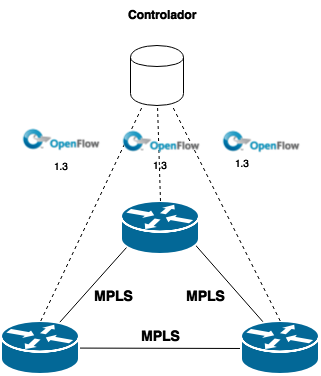
\includegraphics[width=0.4\textwidth]{Arch_Figure0}
\caption[Esquema general del prototipo]{Esquema general del prototipo}
\label{fig:OpenSourceRArch0}
\end{figure}

Por otro lado se tiene el switch compatible con el protocolo OpenFlow. Este dispositivo, denominado de aqu\'i en m\'as \gloss{RAU-Switch}, es implementado mediante una PC de escritorio con el hardware NetFPGA instalado y el software \gloss{Open vSwitch} entre otras componentes.\\ 

Para la implementaci\'on del plano de reenvío (encaminar un paquete de un nodo origen a otro destino), en cada nodo del prototipo se utilizan las tablas de flujos de OpenFlow. Mediante el esquema de flujos de OpenFlow se definen reglas de reenv\'io en base a la conmutaci\'on de etiquetas MPLS, as\'i como pol\'iticas de clasificaci\'on de tr\'afico.\\

De esta forma el prototipo para la RAU2 se compone entonces de unos pocos nodos constru\'idos en base a RAU-Switch y un controlador SDN compatible con OpenFlow, en donde se ejecuta la aplicaci\'on RAUFlow.\\

A continuaci\'on se explica en detalle cada una de estas componentes y su interacci\'on.

\section{RAU-Switch}
Cada nodo en la red prototipo es lo que en este trabajo se denomina RAU-Switch: un switch IP/MPLS h\'ibrido compatible con OpenFlow. Por un lado es un switch OpenFlow dise\~nado en base a dicha arquitectura y por otro lado es un router IP/MPLS puesto que conceptualmente el plano de reenvío es implementado a trav\'es de la conmutación de etiquetas MPLS, mientras que el descubrimiento de la topolog\'ia y la construccui\'on de rutas se basa en algoritmos en base a IP.\\

Debido a que en la literatura OpenFlow es común la denominación de switch OpenFlow a cualquier dispositivo, no importando si en la practica implementa las funcionalidades de un switch de capa dos \'o un router de capa tres, se decidió denominar a esta componente RAU-Switch.\\

\begin{figure}[h] 
\centering    
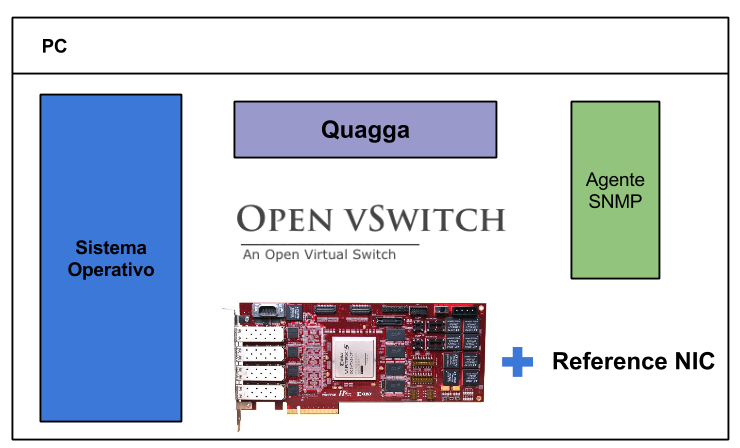
\includegraphics[width=0.7\textwidth]{Arch_Figure1}
\caption[RAU-Switch - diagrama de componentes]{RAU-Switch - diagrama de componentes}
\label{fig:OpenSourceRArch}
\end{figure}

La estructura de este dispositivo esta caracterizada por las componentes que se muestran en la figura~\ref{fig:OpenSourceRArch}. Se utiliza una PC de escritorio como plataforma inicial a la cual se le incorpora una tarjeta NetFPGA-10G programada para que se comporte como una placa de red (proyecto ReferenceNIC) m\'as componentes adicionales de software como Open vSwitch, Quagga y un administrador SNMP. A continuaci\'on se explica en profundidad el rol de cada componente.

\subsection{Plataforma de la PC}
El switch esta constru\'ido sobre la plataforma de una PC de escritorio convencional. En particular se trabaja con un procesador Intel Core i7 de 64 bits, una Mother ASUS ROG Maximus Formula VI, 16GB de memoria DDR3, y un disco HDD de 1TB de capacidad. En el anexo \ref{annexI.1} pueden encontrarse estos detalles con mayor profundidad.

\subsection{Sistema Operativo}
En relación al sistema operativo, se decide trabajar con Ubuntu 12.04 sobre una arquitectura de 64 bits. %Esta elecci\'on responde a dos criterios esencialmente: por un lado la premisa de trabajar con software libre y de c\'odigo abierto preferentemente sugiere la b\'usqueda de un sistema operativo entre alternativas basadas en GNU/Linux; por otro el hardware NetFPGA asi como los proyectos existentes para su programaci\'on fueron desarrollados trabajando sobre la plataforma Fedora14. 

Puesto que la documentaci\'on de la plataforma NetFPGA recomienda el uso del sistema operativo Fedora 14 para trabajar con dicho hardware (la tarjeta NetFPGA 10G fu\'e desarrollada y verificada trabajando sobre esta plataforma), resulta natural trabajar con \'este sistema o al menos una versi\'on superior.\\

En este proyecto se prueban diferentes versiones de esta distribución como Fedora 17 y Fedora 19 adem\'as de la versi\'on ya mencionada, detectando problemas de compatibilidad entre la placa madre y dichas versiones adem\'as de falta de drivers para el cable JTAG.

%Teniendo presente esto, se intenta infructuosamente instalar y configurar el hardware sobre Fedora14. Se prueba con versiones m\'as recientes de la plataforma como Fedora17 y Fedora19 obteniendo los mismos resultados; detectándose entre las causas de error, incompatibilidades entre la placa madre de la PC y las versiones de sistema operativo mencionadas y falta de drivers apropiados para cable JTag utilizado para programar el hardware. 

Tambi\'en se prueban diferentes versiones de la distribuci\'on Ubuntu, logrando en particular instalar y configurar exitosamente el hardware sobre la plataforma Ubuntu 12.04. \\

De esta forma y siguiendo siempre la premisa de trabajar con software libre y c\'odigo abierto se elige Ubuntu 12.04 como plataforma de trabajo.

\subsection{Hardware NetFPGA}

El hardware NetFPGA puede funcionar tanto conectado a una PC por un slot PCIe (modo servidor), como conectado \'unicamente a una fuente de energ\'ia el\'ectrica (modo standalone). En el dise\~no planteado el hardware se encuentra conectado a la PC mediante un slot PCIe; es decir, en modo servidor.

%\subsubsection{Instaaci\'on}
%La tarjeta NetFPGA se encuentra conectada a la PC mediante un slot PCIe. Para programarla, es necesario contar con la suite de Xilinx ISE instalada correctamente, con las respectivas licencias de productos, y un cable de programaci\'on JTAG. En particular, en el prototipo cada router cuenta con la suite de Xilinx ISE instalada, habilitando su reprogramaci\'on. Notar de todos modos que no es estrictamente necesario contar con la suite de Xilinx en el router para su funcionamiento.  

\subsubsection{Herramientas de Programaci\'on}

El hardware puede programarse mediante un cable programador JTAG y la herramienta Impact de la suite de desarrollo de Xilinx ISE SDK. Para ello es indispensable contar con una estaci\'on de trabajo con dichas herramientas instaladas, habilitando la programaci\'on  de la tarjeta NetFPGA que luego ser\'a colocada en la PC de cada nodo. A su vez esta suite se compone por varias herramientas las cuales están licenciadas. Estas licencias adem\'as contemplan la arquitectura del chip Xilinx que en este caso tiene la tarjeta NetFPGA, por ello es indispensable contar con el paquete de licencias apropiado al modelo de chip con que se trabaja (en nuestro caso Virtex5) y a las herramientas utilizadas. 

Esta estaci\'on de trabajo puede o bien ser la propia PC utilizada para el switch (alternativa utilizada en este proyecto) \'o bien puede ser una PC independiente.

%Cabe destacar que en la b\'usqueda de una plataforma compatible para la programaci\'on del hardware se probo con diferentes sistemas operativos como se menciono, logrando programarse el mismo en Windows XP y Ubuntu 12.04.

\subsubsection{Programaci\'on simple}
El hardware puede programarse al menos de dos formas diferentes; una de ellas es lo que aqu\'i se denomina programaci\'on simple. Esta estrategia consiste en la utilizaci\'on de la herramienta Impact y el cable JTAG para grabar en dos chips de la tarjeta (chip FPGA y chip \gloss{CPLD}) dos archivos binarios, uno con la arquitectura de un proyecto y otro con la implementaci\'on del mismo.

Como principales ventajas de esta estrategia se destacan su simplicidad, no requiere de licencias pagas 
 (puede descargarse una licencia gratuita para la herramienta Impact) y adem\'as es el procedimiento que se describe en la documentaci\'on de la plataforma NetFPGA.

No obstante presenta una desventaja importante y es que al producirse un corte de corriente el hardware pierde su programación . Concretamente el contenido del chip FPGA se borrada y solo perdura el contenido del chip CPLD.\\

Tras constatarse este comportamiento, luego de revisar la documentaci\'on de la plataforma y recurrir al foro de la comunidad NetFPGA, se accede a una lista de correos mediante la cual se establece una comunicaci\'on con el equipo de desarrollo de NetFPGA (ver ap\'endice ~\ref{apendiceB2}). Este di\'alogo adem\'as de ayudar en la comprensión del funcionamiento de la plataforma, desemboca en la segunda estrategia de programaci\'on.

\subsubsection{Programaci\'on persistente}
El hardware NetFPGA cuenta en su arquitectura con dos unidades de memoria flash (Flash A y Flash B). En la programaci\'on persistente estas unidades se utilizan para almacenar la programaci\'on del hardware, permitiendo que en cada encendido el chip FPGA sea programado a partir del contenido de una de estas unidades. Por defecto el chip siempre se programa con el contenido de la memoria flash A, habilitando su reprogramaci\'on desde la memoria flash B v\'ia la interfaz PCIe (por mayores detalles de este procedimiento ver ~\citep{PCIEProgProject}).\\

Reprogramar el contenido del chip FPGA en tiempo de encendido, así como también mediante la interfaz PCIe requiere de módulos adicionales tanto en el contenido del chip FPGA, como en el del CPLD. En particular los proyectos ReferenceNIC\citep{ReferenceNICProject}, ReferenceSwitch~\citep{ReferenceSwitchProject} y ReferenceRouter~\citep{ReferenceRouterProject} incorporan estas características.\\

En el procedimiento empleado, inicialmente se programa el hardware con el proyecto ReferenceNIC utilizando la Programaci\'on Simple. Luego es necesario transformar la implementaci\'on del proyecto (archivo bitfile) en un archivo con el formato apropiado para ser almacenado en una de las memorias flash (archivo binario). Esto \'ultimo se realiza utilizando herramientas inclu\'idas en la plataforma de NetFPGA. Finalmente utilizando la herramienta \textbf{pcieprog} también de la plataforma se transfiere el archivo generado a una de las memorias.\\

Cabe destacar que durante la ejecuci\'on de este procedimiento se detectaron algunos errores y comportamientos inesperados en el hardware. Esto fue reportado al equipo de desarrollo de NetFPGA a través de la lista oficial de correos de soporte, reportándose en total dos errores. Luego de este di\'alogo se obtiene una soluci\'on a dichos errores los cuales cabe destacar que son contemplados y resueltos en la siguiente actualizaci\'on del repositorio de c\'odigo fuente. Por m\'as detalles acerca de estos errores y la forma en que son resueltos provisoriamente referirse al ap\'endice~\ref{apendiceA}.\\

Otro detalle a destacar de esta estrategia, es la utilizaci\'on de herramientas de la suite de Xilinx que requieren de licencias especiales con un costo ecnon\'omico considerable. En relaci\'on a este aspecto en el marco de este proyecto se solicit\'o asesoramiento al Instituto de Ingeniería Eléctrica de la Facultad de Ingenieria (IIE) adem\'as de solicitar una donaci\'on a trav\'es del programa de apoyo universitario de Xilinx. Por mayores detalles acerca de este problema puede consultarse el apéndice ~\ref{apendiceB3}

%En el marco de este proyecto se solicita apoyo en relaci\'on a este tema a docentes del Instituto de Ingeniería Eléctrica de la Facultad de Ingenieria 
 %(IIE) y a través del programa de apoyo universitario de Xilinx, en busca de una soluci\'on a este problema.

%Si bien en el IIE no se trabaja con esta plataforma se obtiene de parte de este instituto asesoramiento sumamente \'util para la resoluci\'on de este obstáculo. Por otro lado a través del programa de apoyo a universidades de Xilinx se obtiene una interesante donaci\'on de licencias, posibilitando a una real explotaci\'on del hardware y de la plataforma. Por mayores detalles acerca de este problema puede consultarse el apéndice ~\ref{apendiceB3}.

\subsection{Open vSwitch}
En la arquitectura del dispositivo, Open vSwitch es el encargado de implementar el plano de datos de OpenFlow. En otras palabras es la componente que convierte al nodo construido en un switch OpenFlow, mediante una implementaci\'on en software.\\

Siguiendo la especificaci\'on de OpenFlow, Open vSwitch implementa el concepto de tabla de flujos. Estas tablas (Open vSwitch implementa 256 tablas) son utilizadas por la aplicaci\'on RAUFlow para construir caminos en la topolog\'ia, instalando en forma de flujos OpenFlow las reglas de reenvío que sean necesarias en cada nodo involucrado en un camino.

Para implementar el plano de reenvío en base a la conmutaci\'on de etiquetas MPLS, se utilizan primitivas del protocolo OpenFlow, que permiten colocar y extraer etiquetas MPLS de un paquete (PUSH y POP), así como clasificar un paquete acorde al valor de la etiqueta MPLS contenida en \'el.\\

Vale la pena destacar en relaci\'on a este \'ultimo punto, que la documentaci\'on de la herramienta presenta inconsistencias entre algunas de las funcionalidades declaradas y las realmente implementadas. En particular la manipulaci\'on de etiquetas MPLS no esta completamente soportada. Por mayores detalles en relaci\'on a estos aspectos y la resoluci\'on de otros problemas detectados al trabajar con esta herramienta referirse al ap\'endice ~\ref{apendiceB5}.
 
%En relaci\'on a este \'ultimo punto, vale la pena destacar que la compatibilidad con estas funcionalidades del protocolo OpenFlow, están acotadas naturalmente  por la implementaci\'on de Open vSwitch. En este trabajo inicialmente se utiliza la versi\'on oficial m\'as reciente de dicha herramienta (versi\'on 2.3.1), en la cual acorde a las notas de liberaci\'on y a la secci\'on de preguntas frecuentes se garantiza soporte para solo un subconjunto de funcionalidades de la versi\'on 1.3 del protocolo OpenFlow. Entre estas funcionalidades se destacan la capacidad para match, push y pop de una \'unica etiqueta MPLS, así como su posterior procesamiento en el pipe de OpenFlow. No obstante como se explica en el apéndice ~\ref{apendiceB5} junto a otras características a destacar de Open vSwitch, este comportamiento no es el que realmente manifiesta esta versi\'on de la herramienta. En particular la operación Pop de MPLS no funciona correctamente, así como el posterior procesamiento del paquete tras manipular etiquetas acorde al pipe de OpenFlow.\\ 

%Afortunadamente esta falla se encuentra reportada como error y es resuelta en la versi\'on de desarrollo~\citep{OVSSourceCode}, la cual a su vez tras instalarse se comprueba que soporta match, push y pop de hasta tres etiquetas mpls, junto el posterior procesamiento del paquete. De esta forma la versi\'on de Open vSwitch utilizada es la de desarrollo.\\

Por otro lado, resulta interesante a tener en consideraci\'on que las operaciones de Match, Push y Pop de MPLS son implementadas en modo usuario, con una considerable penalizaci\'on en rendimiento en comparaci\'on a una implementaci\'on en modo Kernel.

%Por otro lado en relaci\'on a las componentes de software, el router se compone de un sistema operativo escritorio basado en linux, con las instalaciones de Open vSwitch, Quagga y el agente de gesti\'on SNMP. Nuevamente por mayores detalles acerca de las versiones de software utilizadas, sistema operativo entre otros detalles refierase al anexo [link al anexo].\\

\subsection{Quagga}
En cada nodo se ejecuta una instancia del software de enrutamiento Quagga, configurada para ejecutar el demonio Unix OSPF.\\ 

Este demonio Unix, ejecuta el protocolo de igual nombre, utilizado en la arquitectura propuesta para obtener información de cada nodo y sus adyacencias en la topolog\'ia, guardando dicha información en una base de datos local (Link-State-Database o \gloss{LSDB}). Entre los datos que se incluyen en esta base de datos topol\'ogica se destaca el costo asociado a cada adyacencia.\\ 

Como se menciona anteriormente, el algoritmo OSPF se utiliza solamente para la construcci\'on de la base de datos topol\'ogica. Si bien en un inicio se pensó en trabajar con la salida de dicho algoritmo, finalmente se decidió trabajar con el algoritmo de ruteo centralizado implementado en el controlador. Por ello en la versi\'on final del prototipo no se utiliza la salida de este algoritmo a pesar de que la arquitectura permite su utilización para alimentar la entrada de procesos que se ejecuten en el controlador.\\

De esta forma cada switch del prototipo así como el propio controlador ejecuta una instancia de Quagga con el demonio Unix OSPF configurado como se muestra en el apéndice \ref{appendix4}. Cabe destacar de dicha configuración que la adyacencia entre un switch y el Controlador (enlace utilizado para el canal de comunicación OpenFlow) tiene asociado costo infinito para evitar que sea utilizado tanto por el algoritmo OSPF como por el algoritmo CSPF en la construcción de algún camino. En la implementaci\'on de Quagga el costo infinito es representado por el numero 65535 (16 bits).

\subsection{Agente SNMP}
El protocolo de comunicación OpenFlow dentro de las estructuras de datos utilizadas para el intercambio de información entre un switch y el Controlador, no prevee una forma de comunicar el direccionamiento IP propio del equipo (direcciones IP de cada interfaz física). En particular la estructura \textit{ofp\_port} utilizada por el mensaje \textit{OFPMP\_PORT\_DESCRIPTION} no provee de dicho campo (ver especificación del protocolo OpenFlow 1.3\citep{ofv133spec}). Por esta razón es necesaria una forma de comunicar al controlador información adicional sobre características de cada nodo como la dirección IP de una interfaz, que no puede ser enviada a través del protocolo OpenFlow. Para evitar modificar el protocolo extendiéndolo para comunicar dicha informaci\'on, se utiliza un agente SNMP.\\

SNMP definido a través de los RFC1065~\citep{rose1990structure} y RFC1157~\citep{case1989simple} entre otros, es un protocolo que permite intercambio de información entre dispositivos de red y una entidad administradora. Para su despliegue en una red son necesarias tres componentes: 

\begin{enumerate}

\item Dispositivo administrado: Es el dispositivo de red que se quiere monitorizar.

\item Agente: Es el software que se ejecuta en el dispositivo administrado y se encarga de comunicarse mediante el protocolo con el sistema administrador de red.

\item Sistema administrador de red: El dispositivo que se encargara de realizar las consultas sobre la información deseada a los dispositivos administrados.

\end{enumerate}	

En el prototipo se instala un agente SNMP en cada switch (dispositivo administrado), para enviar la correspondencia entre números de puerto OpenFlow y direcciones IP al Controlador (sistema administrador).\\

No es el objetivo de este trabajo entrar en detalle sobre el protocolo SNMP por lo que si el lector desea profundizar en estos conceptos se recomienda seguir las referencia mencionadas anteriormente.

\section{Entidad Controlador}
Como se muestra en \ref{fig:OpenSourceRArch0} cada nodo del prototipo responde a una entidad denominada Controlador. Esta entidad en la pr\'actica es una PC convencional con determinadas componentes de software (ver figura \ref{fig:OpenSourceRArch3}) entre las cuales se destaca el controlador SDN Ryu, pilar fundamental en la implementaci\'on de la aplicaci\'on RAUFlow. A su vez se encuentran los módulos Administrador SNMP utilizado en la comunicaci\'on con los agentes SNMP instalados en cada nodo RAUSwitch y LSDBSync utilizado en el proceso de extracci\'on de informaci\'on de la base de datos topol\'ogica de Quagga. 

Estas tres componentes se ejecutan en una PC de escritorio con Ubuntu 12.04 como sistema operativo. \\

\begin{figure}[h] 
\centering    
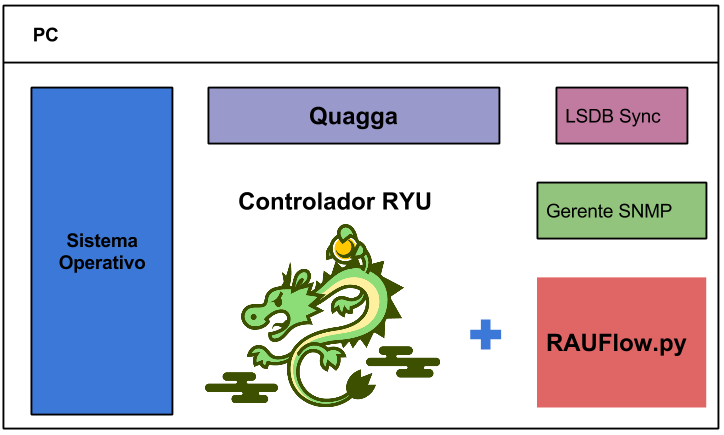
\includegraphics[width=0.6\textwidth]{Arch_Figure3}
\caption[Diagrama de componentes del Controlador]{Diagrama de componentes del Controlador}
\label{fig:OpenSourceRArch3}
\end{figure}

A continuación se explica en detalle cada una de las tres componentes mencionadas.

\subsection{Controlador Ryu}
Ryu es la alternativa de software elegido para implementar el controlador SDN compatible con el protocolo OpenFlow. 

Utilizando esta herramienta para la construcci\'on y ejecuci\'on de una o m\'as aplicaciones SDN, se implementa prácticamente la totalidad del plano de control del prototipo. Esto es en otras palabras la implementaci\'on del modelado de la realidad, la implementaci\'on de funcionalidades para la creaci\'on de servicios de redes privadas, implementaci\'on de cliasficiaci\'on de tr\'afico y eventualmente la implementaci\'on de pol\'iticas de ingenieria de tr\'afico y calidad de servicios (QoS).\\ 

Dada la complejidad en el diseño y arquitectura de esta componente, se destina el próximo cap\'itulo a la explicaci\'on de las diferentes características e implementaci\'on de las aplicaciones Ryu que constituyen el plano de control del prototipo, as\'i como la interacci\'on de las otras componentes mencionadas dentro del plano de control como los m\'odulos LSDBSync y Administrador SNMP. 

\subsection{Quagga}
El controlador ejecuta una instancia de Quagga, obteniendo de esta forma acceso local a la información de la base de datos topol\'ogica construida por OSPF (Link-State-Database), una vez que el algoritmo converge.

Para obtener esta informaci\'on y detectar cambios la topolog\'ia se utiliza el m\'odulo LSDB Sync.

\subsection{LSDB Sync}
LSDB Sync se encarga de tomar la información de la base de datos topol\'ogica una vez que el algoritmo OSPF converge, procesarla y enviarla a las aplicaciones que se ejecutan en el controlador.\\

Esta componente consta de dos módulos. El primero se encarga de escuchar los mensajes del protocolo enviados por Quagga, generando un evento cuando el mismo converge, luego de producirse un cambio en la topolog\'ia; el cual luego es tomado por el segundo m\'odulo.

Una vez capturado el evento anterior, el segundo m\'odulo toma la información topol\'ogica en la base local del controlador y la procesa para ser enviada a las aplicaciones en el controlador.

Luego se produce un proceso de actualizaci\'on topol\'ogica, en el que eventualmente el controlador utilizando el m\'odulo Administrador SNMP obtiene informaci\'on adicional sobre los dispositivos del prototipo. 

\begin{subsection}{Administrador SNMP}
El administrador SNMP es utilizado para consultar al agente SNMP instalado en un nodo, por la correspondencia entre números de puerto OpenFlow y direcciones IP. Esta componente es utilizada por las aplicaciones en el Controlador cada vez que es preciso obtener esta información de mapeo para un nodo (por ejemplo en el proceso de actualización de la topolog\'ia).\\\\\

\end{subsection}

En resumen, los nodos del prototipo son construidos en base al hardware NetFPGA y una PC convencional a la cual se le instalan diferentes componentes de software de forma de implementar un switch MPLS/OpenFlow. Luego el plano de control de la red se implementa en una PC con el software controlador Ryu instalado m\'as un conjunto de m\'odulos adicionales.

%En resumen, el prototipo se compone de nodos construidos en base al hardware NetFPGA y una PC convencional el la cual se instalan diferentes componentes de software de forma de implementar un switch MPLS/OpenFlow. Luego una PC normal en la que se instala el controlador Ryu m\'as un conjunto de m\'odulos adicionales. Como se muestra en la figura\ref{fig:OpenSourceRArch4}, luego la comunicación entre cada par de nodos es IP/MPLS, mientras que cada nodo es manipulado por el protocolo OpenFlow. Adicionalmente se tiene un canal IP entre cada nodo y el plano de control por donde se comunican cada agente SNMP con el administrador.

\begin{figure}[h] 
\centering    
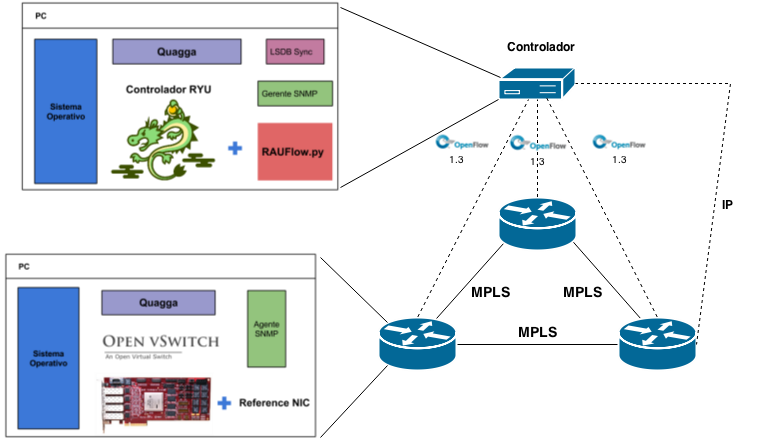
\includegraphics[width=0.9\textwidth]{Arch_Figure4}
\caption[Vista l\'ogica ampliada del prototipo]{Vista l\'ogica ampliada del prototipo}
\label{fig:OpenSourceRArch4}
\end{figure}

En el siguiente cap\'itulo se explica en detalle el proceso de diseño e implementaci\'on de la aplicaci\'on RAUFlow, as\'i como la interaci\'on con las diferentes componentes de RAUSwitch.

%\chapter{RAUFlow}
\label{Capítulo 5}

% **************************** Define Graphics Path **************************
\ifpdf
    \graphicspath{{Chapter5/Figs/Raster/}{Chapter5/Figs/PDF/}{Chapter5/Figs/}}
\else
    \graphicspath{{Chapter5/Figs/Vector/}{Chapter5/Figs/}}
\fi

En cap\'itulos anteriores se ha detallado las caracter\'isticas m\'as importantes del prototipo, as\'i como las principales componentes del router opensource y la entidad Controlador. 
Resta detallar el dise\~no de la aplicaci\'on a ejecutarse en el Controlador, y encargada de implementar el plano de control del prototipo; de aqu\'i en m\'as RauFlow. Por ello en el presente cap\'itulo se propone un an\'alisis de dicha componente, siguiendo un proceso de dise\~no tradicional de Ingenier\'ia de Software, dividido en 4 etapas. Una primera etapa de an\'alisis de requerimientos, una segunda etapa de relevamiento de casos de uso, una tercera etapa de dise\~no del modelo de datos, y finalmente una cuarta etapa para el dise\~no general de la arquitectura de la aplicaci\'on. Finalmente se presentan los aspectos m\'as importantes relacionados a la implementaci\'on de RAUFlow, como por ejemplo las implementaciones de un algoritmo de ruteo din\'amico y de un algoritmo de distribución de etiquetas. 

\section[An\'alisi de requerimientos]{An\'alisis de requerimientos}

Anteriormente en ~\ref{section1.2.2} se definieron algunos de los requerimientos relevados para el prototipo de la RAU. De ellos y de un trabajo de an\'alisis sobre la realidad modelada, se desprende la siguiente tabla de requerimientos para RauFlow:

\clearpage
\begin{table}[Htl]\centering
\begin{tabularx}{\textwidth}{|>{\setlength\hsize{1.0\hsize}\setlength\linewidth{\hsize}}X|}
\hline
Requerimientos Funcionales\\ \hline
\hline
\begin{itemize}
\item El Sistema debe de proveer la facilidad para obtener la informaci\'on asociada a cada nodo de la red, permitiendo a su vez agregar informaci\'on que facilite la identificaci\'on del mismo para un usuario.
\item El Sistema debe proveer la facilidad para agregar, modificar y eliminar redes virtuales. 
%En particular al trabajar con redes virtuales y sus datos, se debe soportar el manejo de datos como la numeraci\'on IP del tr\'afico asociado a una red virtual, informaci\'on de capa de transporte, entre otros.
\item El Sistema debe proveer la facilidad para obtener toda la informaci\'on relevante de una red virtual.
\item El Sistema debe permitir visualizar de alguna forma los caminos constru\'idos para encaminar el tr\'afico de una red virtual en particular, a trav\'es de la red del protot\'ipo.
\item El Sistema debe proveer la facilidad para visualizar el estado de las tablas de flujos asociadas a cualquier nodo de la red del protot\'ipo.
\end{itemize}\\
\hline
\end{tabularx}
\end{table}

\begin{table}[Htl]\centering
\begin{tabularx}{\textwidth}{|>{\setlength\hsize{1.0\hsize}\setlength\linewidth{\hsize}}X|}
\hline
Requerimientos no Funcionales\\ \hline
\hline
\begin{itemize}
\item Se debe utilizar siempre que sea posible herramientas de software libre y c\'odigo abierto.
\end{itemize}\\
\hline
\end{tabularx}
\end{table}

Teniendo en cuenta la descripci\'on del problema y los requerimientos anteriores, se procedio con el modelado de la realidad. Los resultados obtenidos se presentan en la siguiente secci\'on.

%Teniendo en cuenta los requerimientos anteriores, se procede con el relevamiento de los casos de uso. Los resultados obtenidos se presentan en la siguiente secci\'on.

\section[Modelado de la realidad]{Modelado de la realidad}

En la figura ~\ref{fig:ModeloDeDominio} se presenta el modelo de dominio realizado a partir de la realidad planteada. En el mismo se destacan en color amarillo aquellas entidades que se entiende se corresponden al modelado de los elementos de la topolog\'ia como lo son Nodos e Interfaces. Por otro lado en rosado se destacan aquellas entidades relacionadas al concepto MPLS que se consideran importantes, como lo son las tablas FTN, ILM y NHLFE. Finalmente vale la pena destacar el concepto de Servicio, con el cual se decidi\'o representar a las redes virtuales soportadas en el protot\'ipo. Interesa destacar adem\'as del concepto de Servicio, que es una redefinici\'on desde una visi\'on centralizada del concepto FEC en la teor\'ia de MPLS, concepto que en la literatura de MPLS tradicional esta vinculado a un solo nodo en una red, y no a muchos como se propone en este trabajo.  

\begin{figure}[ht!] 
\centering    
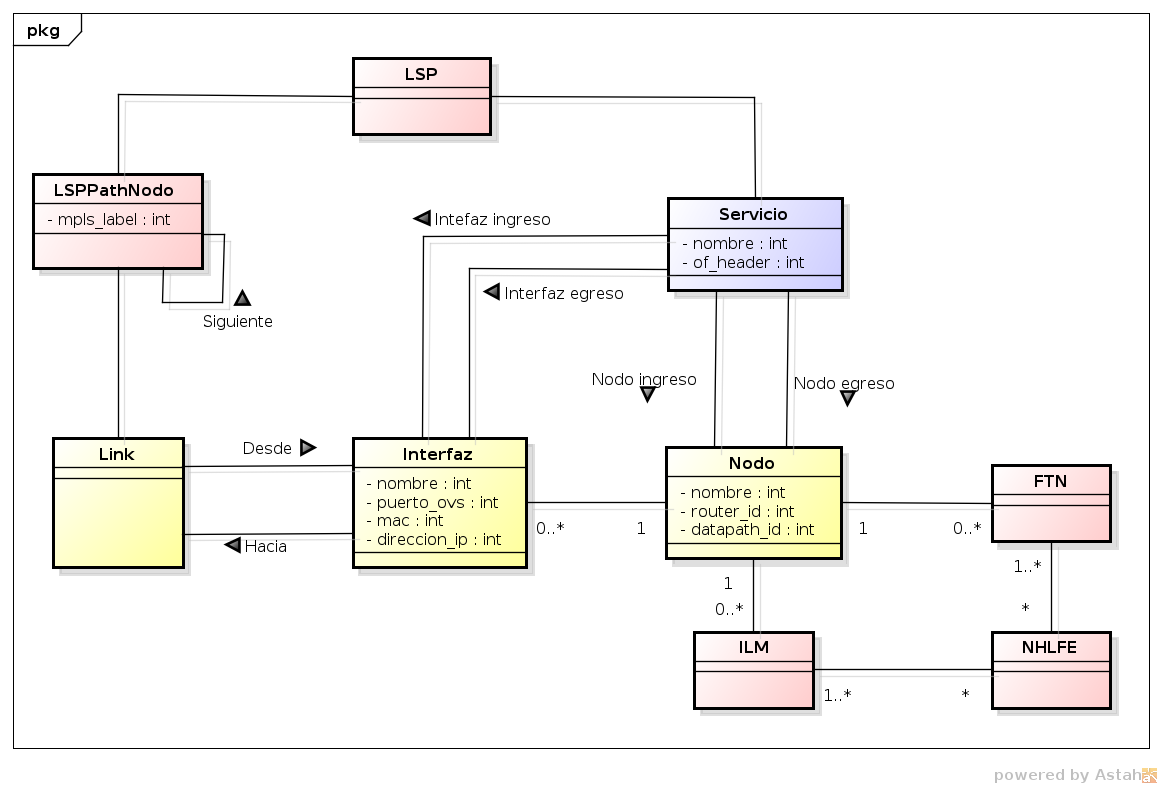
\includegraphics[width=0.7\textwidth]{Disenio_Figure1}
\caption[ModeloDeDominio]{Modelo de Dominio}
\label{fig:ModeloDeDominio}
\end{figure}

Sobre este modelo de dominio se trabaj\'o hasta llegar finalmente al diagrama de clase de dise\~no que se presenta a continuaci\'on en la figura [ref].\\

Teniendo en cuenta los requerimientos mencionados, y el modelado de la realidad presentado, se procede con el relevamiento de los casos de uso. Los resultados obtenidos se presentan en la siguiente secci\'on.

\section[Relevamiento de casos de uso]{Relevamiento de casos de uso}

La lista de casos de uso presentada a continuaci\'on se corresponde con un conjunto de funcionalidades b\'asicas, que permiten la exploraci\'on de la potencialidad del enfoque SDN aplicado al problema planteado. 

\begin{itemize}
\item Listar Servicios
\item Agregar Servicio
\item Modificar Servicio
\item Eliminar Servicio
\item Ver Topolog\'ia
\item Ver informaci\'on b\'asica Nodo
\item Ver tabla de Flujos Nodo
\item Filtrar Lsps
\item Editar Informaci\'on extra Nodo
\item Editar Informaci\'on extra Interfaz
\end{itemize}

%De esta forma quedan presentados los requerimientos relevados sobre RauFlow, el modelado de la realidad, y los casos de uso relevados. Resta entonces presentar un esbozo de la arquitectura de la aplicaci\'on RauFlow, para que el lector finalmente este en condiciones de comprender el dise\~'no del prototipo en su totoalidad.
\section[Arquitectura de RauFlow]{Arquitectura de RauFlow}

En esta secci\'on se presenta la arquitectura de la aplicación RauFlow(ver figura ~\ref{fig:VistaComponentes2}), profundizándose en el funcionamiento de sus principales componentes.\\

Como se muestra en la figura\ref{fig:VistaComponentes2}, RauFlow esta basado principalmente en una aplicaci\'on Ryu(RauFlowApp) y un conjunto de aplicaciones Ryu adicionales.\\ 

Con el objetivo de mantener simple y modular el dise\~no de RauFlow, se implementa en RauFlowApp solamente aquellas funcionalidades y responsabilidades asociadas al protocolo OpenFlow y sus respectivos eventos. Luego responsabilidades y funcionalidades asociadas a la realidad modelada y sus reglas de negocios, son delegadas a una capa de negocios. Ademas se tiene un conjunto de aplicaciones Ryu dise\~nadas e implementadas por terceros, las cuales se encuentran dentro del conjunto de aplicaciones que vienen con el software Ryu. M\'as adelante se explicar\'a en detalle cual es el rol que cumplen estas aplicaciones en el dise\~no de RauFlow.

Para completar esta visi\'on general de RauFlow, se incluye en su arquitectura una interfaz de usuario gr\'afica.\\ 

%Como se explico anteriormente, Ryu habilita la programaci\'on del plano de control mediante aplicaci\'ones desarrolladas en lenguaje Phyton con una cierta estructura particular. Por consiguiente RauFlow esta basado en al menos una aplicaci\'on de este tipo.\\

%Por otro lado si bien Ryu ofrece un entorno para la ejecuci\'on de m\'ultiples aplicaciones, asi como un mecanismo para la comunicaci\'on entre ellas, por simplicidad se opta por basar el dise\~no de RauFlow en una \'unica aplicaci\'on Ryu lo m\'as simple posible. Luego funcionalidades y responsabilidades que no son previstas en dicha aplicaci\'on son implementadas por componentes adicionales, siguiendo un dise\~no modular.\\

%Cabe destacar adem\'as, la existencia en el dise\~no de un conjunto de aplicaciones Ryu, dise\~nadas e implementadas por terceros. Estas aplicaciones en particualr se encuentran dentro del conjunto de aplicaciones que vienen con el software Ryu. M\'as adelante se explicar\'a en detalle cual es el rol que cumplen estas aplicaciones en el dise\~no de RauFlow.\\

En res\'umen, el dise\~no de RauFlow se caracteriza por una arquitectura en cuatro capas: (1) capa de presentación, (2) capa de aplicaciones Ryu, (3) capa de negocios, y (4) capa de dispositivos.\\

\newpage
\begin{figure}[ht!] 
\centering    
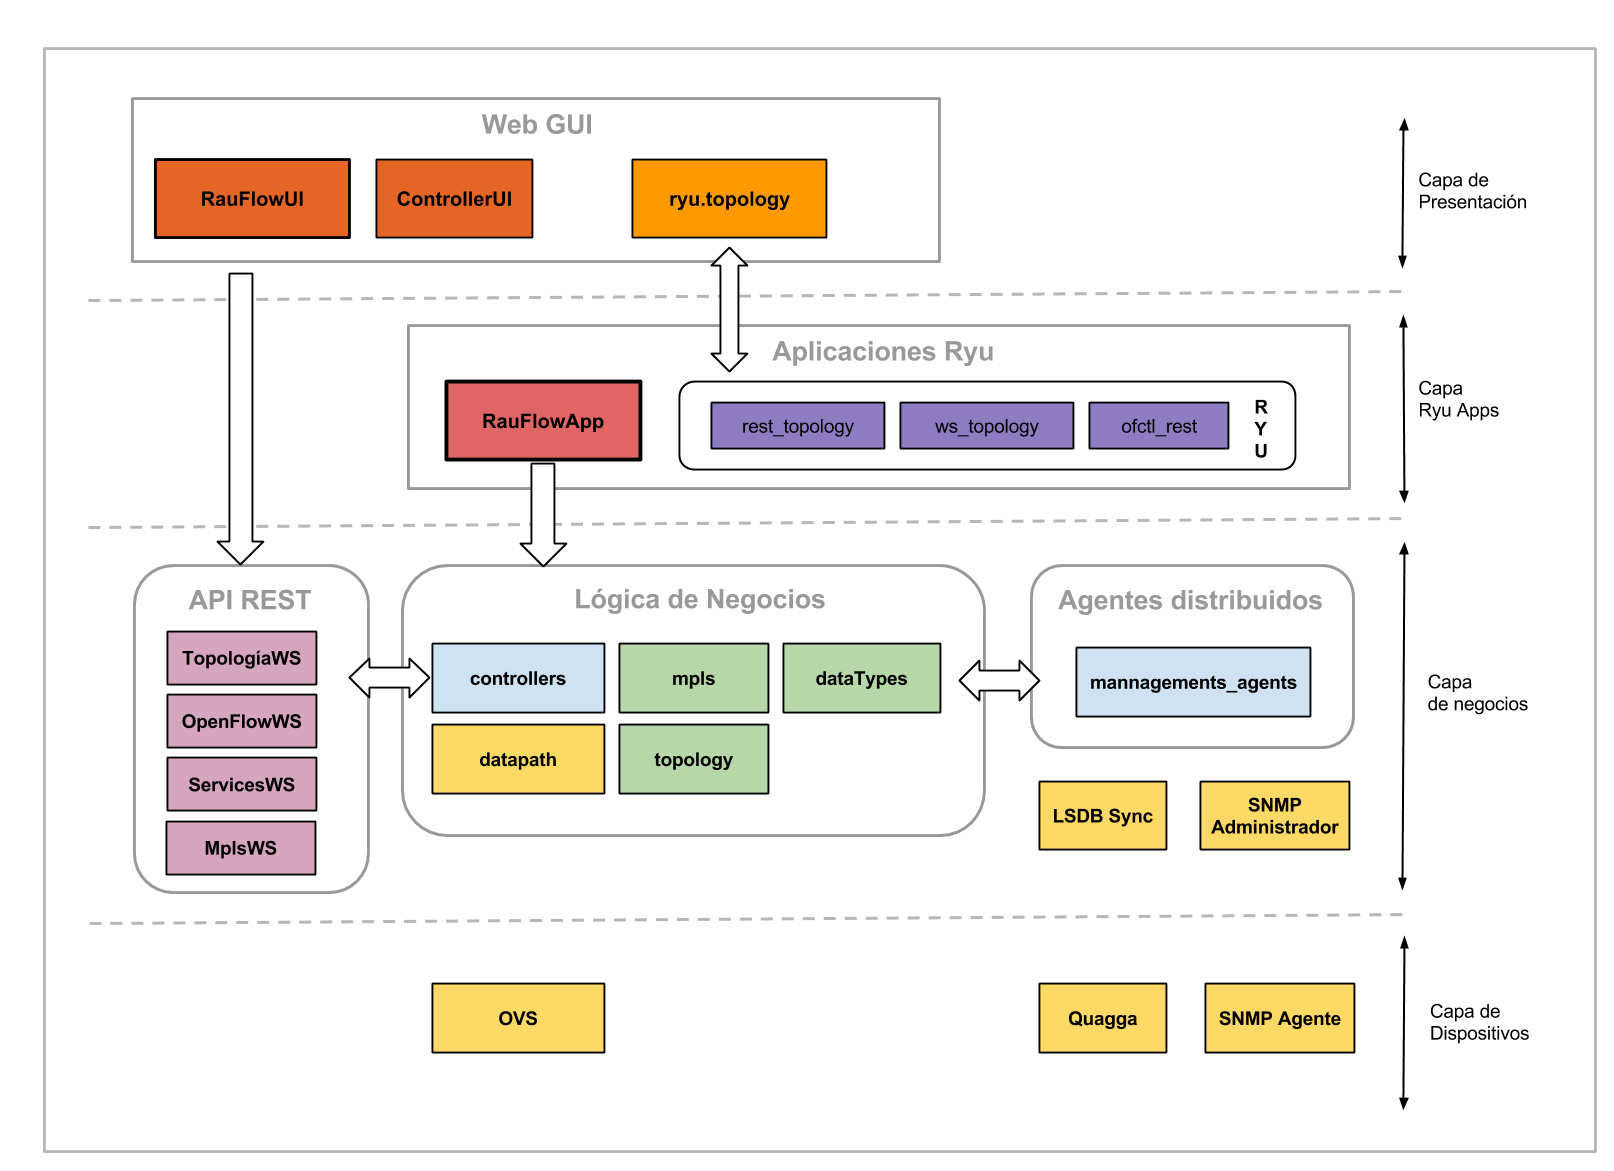
\includegraphics[width=1.0\textwidth]{Disenio_Figure3}
\caption[Vista l\'ogica]{Vista l\'ogica}
\label{fig:VistaComponentes2}
\end{figure}

\subsection{Capa de aplicaciones Ryu}
En esta capa se encuentran las diferentes aplicaciones Ryu que conforman al prototipo. Como se menciona anteriormente, RauFlow esta compuesto por una aplicaci\'on de autoria propia, y tres aplicaciones de terceros(incluidas en las aplicaciones que vienen con el software de controlador).\\

La aplicaci\'on RauFlowApp es la encargada de implementar el plano de control en el prototipo; por lo tanto, a priori su alcance puede ser tan grande como el propio alcance de RauFlow. Esto redunda en una complejidad mayor en el dise\~no de la misma. Por esta razón se decide desacoplar las reglas de negocio de la realidad, de dicha aplicación. De esta forma se genera la mencionada capa de negocios; en donde se coloca todo este conocimiento de la realidad modelada, reglas de negocio, y funcionalidades.  

\subsubsection{Aplicaciones de terceros}
Ryu incluye tres aplicaciones dise\~nadas para implementar una interfaz gr\'afica. Dicha interfaz consiste en un p\'agina web implementada sobre html, javascript y web sockets, que permite visualizar la red en su totalidad. Estos son los dispositivos del datapath con sus interfaces, y los enlaces existentes.

Por esta razon se incluyen en el dise\~no del proptotipo dichas aplicaciones, agregando funcionalidades  a la capa de presentaci\'on, y reutilizando desarrollos existentes.

\subsection{Capa de Negocios}
La capa de negocios presenta tres componentes bien definidas: una componente de reglas y l\'ogica de negocios de la realidad, una API REST de servicios para el acceso y la manipulaci\'on de datos relacionados a la primera componente, y una tercera componente denominada Agentes distribu\'idos.

\subsubsection{Lógica de Negocios}
La componente lógica de negocios se subdivide en diferentes m\'odulos que agrupan funcionalidades acorde a su naturaleza y responsabilidades. Vale la pena destacar a su vez que cada uno de estos m\'odulos se corresponde en la implementaci\'on con un package en la nomenclatura de Python. Estas funcionalidades y responsabilidades se corresponden de la siguiente forma:

\begin{itemize}
\item \textbf{controller:} Este m\'odulo agrupa diferentes controladores de objetos. Actualmente contiene un \'unico controlador façade, responsable de mantener el \'unico punto de acceso a la las componentes de la l\'ogica de negocios. Contiene desde la implementaci\'on de funciones para dar de alta Servicios, crear LSPs, obtener el mejor camino entre dos nodos de la red, etc.

\item \textbf{topology:} Agrupa las definiciones de objetos utilizados para representar la topolog\'ia como las clases Nodo, Interfaz y Link, así como otros conceptos de la realidad.
 
\item \textbf{mpls:} Contiene las definiciones de los conceptos FTN, ILM, NHLFE(rectificar esto xq esta en topology actualmente), as\'i como el conceptos de Servicio ya explicado anteriormente, y de LSP(label switched path).

\item \textbf{dataTypes:} Mantiene representaciones reducidas de los principales objetos definidos en todos los m\'odulos de la componente de negocios, para el intercambio de datos con por ejemplo la capa de presentaci\'on. 

\item \textbf{datapath:} Agrupa funcionalidades para el acceso al datapath de OpenFlow, como funciones para agregar y eliminar flujos en un switch, u obtener estad\'isticas de una tabla de flujos.
\end{itemize} 

\subsubsection{API REST de servicios}
La componente de Servicios REST, se encuentra subdividida en varios m\'odulos respondiendo al criterio utilizado para el dise\~no modular de la componente de l\'ogica de negocios. [De repente podemos poner como anexo la especificacion de la api para que se vean las funcionalidades que tiene].

\subsubsection{Agentes distribuidos}
Esta componente es la encargada de la interacci\'on con diferentes agentes y procesos instalados en cada router opensource a través de un canal de comunicación IP. Este m\'odulo de comunicaci\'on, as\'i como los diferentes agentes instalados en cada router opensource, juegan un rol irreemplazable en la obtenci\'on de informaci\'on adicional sobre cada nodo; puesto que a partir del canal de comunicaci\'on OpenFlow solamente es accesible Open vSwitch y la informaci\'on contemplada por el protocolo OpenFlow.

Dentro de esta componente, en el diagrama se muestra un modulo denominado \textbf{managements\_ agents}. Este m\'odulo opera como una interfaz de conexi\'on entre los diferentes m\'odulos de la l\'ogica de negocios, y los diferentes m\'odulos que implementan la comunicaci\'on con su respectivo agente distribu\'ido.

En la figura ~\ref{fig:VistaComponentes2} se muestran el modulo \textbf{SNMP Management}, responsable de  la comunicaci\'on con un agente SNMP distribu\'ido entre los nodos del prototipo, con el fin de obtener informaci\'on extra acerca de las interfaces de red de cada router opensource.\\

\subsection{Capa de Presentación}
Dentro de la capa de presentaci\'on se destacan: (1) una interfaz gr\'afica identificada en el esquema como RauFlowUI, la cual implementa cada uno de los casos de uso mencionados anteriormente en [link a la secci\'on de casos de uso], (2) ControladorUI, componente que funciona como nexo entre las funcionalidades de RauFlowUI y la API Rest de Servicios, y (3) \textbf{ryu.topology}. Esta \'ultima componente forma parte del conjunto de apliaciones Ryu adicionales que se incluyen en el dise\~no de RauFlow, y tiene como principal funci\'on la de proveer una representaci\'on gr\'afica en tiempo real de la topolog\'ia existente en el prototipo.\\

\section[Implementaci\'on]{Implementaci\'on}

En esta secci\'on se presentan los aspectos m\'as importantes en relaci\'on a la implementaci\'on de RauFlow. Entre ellos se destacan la presentaci\'on del algoritmo de ruteo din\'amico implementado, el algoritmo de distribusi\'on de etiquetas, las convenciones utilizadas para identificar y crear clases de servicios, entre otros.\\

\subsection{Implementación de Servicio}

En la realidad modelada se tienen dos conceptos fundamentales asociados a una red privada virtual (VPN): (1) el concepto de servicio y (2) el concepto de calidad de servicio.

\begin{enumerate}
\item El concepto de servicio establece un trato diferencial para el tr\'afico asociado a una VPN, bajo ciertas condiciones bien definidas(tipicamente temporales). 
\item El concepto de calidad de servicio (QoS), establece características sobre el procesamiento del trafico en la red(tipicamente reserva de ancho de banda) que repercuten luego en el calculo del camino a seguir por dicho trafico.
\end{enumerate}

En relación al concepto de servicio, en la perspectiva que se adopta en RauFlow presenta las siguientes  características:

\begin{itemize}
\item Es un concepto global que involucra a toda la topolog\'ia
\item Queda determinado parcialmente por la cuádrupla 
\begin{center}
(nodo\_ingreso, interfaz\_ingreso, nodo\_egreso, interfaz\_egreso)
\end{center}
\item Interesa distinguir servicios utilizando las capacidades provistas por los matching fields de OpenFlow 
\item Esta definido temporalmente (para un rango horario espec\'ifico)[esto no se si lo ponemos]
\end{itemize}

De esta forma el concepto de servicio se define mediante la clase Servicio como se muestra a continuación.

\begin{python}
class Service(object):

		#General attributes
		ID 				    #str(uuid.uuid4()) Unique ID 
		name 				#Service name for clear 
							#identification by RauFlow users
							
		lsps				#List of services lsps
		
		ingress_node		#Ingress node of service traffic 
							#in the core
							
		egress_node 		#Egress node of service traffic 
							#in the core
							
		ingress_interface 	#Ingress interface of the service 
							#traffic in the ingress node
							
		egress_interface 	#Egress interface of the service 
							#traffic in the egress node
        
		#Attributes from OFv1.3 matching fields
		in_port			# Switch input port.
		in_phy_port 	# Switch physical input port. 
		metadata 		# Metadata passed between tables. 
		eth_dst 		# Ethernet destination address.
		eth_src 		# Ethernet source address. 
		eth_type 		# Ethernet frame type. 
		vlan_vID 		# VLAN id. 
		vlan_PCP		# VLAN priority. 
		IP_dscp 		# IP DSCP (6 bits in ToS field). 
		IP_ecn  		# IP ECN (2 bits in ToS field). 
		IP_proto		# IP protocol. 
		IPv4_src 		# IPv4 source address. 
		IPv4_dst 		# IPv4 destination address. 
		TCP_src 		# TCP source port. 
		TCP_dst 		# TCP destination port. 
		UDP_src 		# UDP source port. 
		UDP_dst 		# UDP destination port. 
		SCTP_src 		# SCTP source port. 
		SCTP_dst 		# SCTP destination port. 
		ICMPv4_type 	# ICMP type. 
		ICMPv4_code 	# ICMP code. 
		ARP_op			# ARP opcode. 
		ARP_spa 		# ARP source IPv4 address. 
		ARP_tpa 		# ARP target IPv4 address. 
		ARP_sha 		# ARP source hardware address. 
		ARP_tha 		# ARP target hardware address. 
		IPv6_src 		# IPv6 source address. 
		IPv6_dst 		# IPv6 destination address. 
		IPv6_flabel 	# IPv6 Flow Label 
		ICMPv6_type 	# ICMPv6 type. 
		ICMPv6_code 	# ICMPv6 code. 
		IPv6_nd_target 	# Target address for ND. 
		IPv6_nd_ssl 	# Source link-layer for ND. 
		IPv6_nd_tll  	# Target link-layer for ND. 
		MPLS_label 		# MPLS label. 
		MPLS_tc 		# MPLS TC. 
		MPLS_bos		# MPLS BoS bit. 
		PBB_is_id 		# PBB I-SID. */
		tunnel_id 		# Logical Port Metadata. 
		IPv6_txhdr 		# IPv6 Extension Header pseudo-field 
		
\end{python}

En cuanto a como se implementan las nociones de calidad de servicio, se detallan m\'as adelante en~\ref{5.5.4} 

\subsection{Algoritmo de distribución de etiquetas}
Tradicionalmente, en mpls se utilizan etiquetas para: (a) asociar trafico a una VPN en particular y (b) encaminar trafico en la red(reenvío en base a etiquetas). De esta forma se tienen dos niveles de etiquetas: un primer nivel(inner label) utilizado para asociar el trafico con la VPN y asi por ejemplo aplicar localmente políticas de QoS, y el segundo nivel (outer label) utilizado para construir el LSP(label switched path).\\

Para la distribución de etiquetas(inner y outer label) existen protocolos entre los cuales se puede destacar LDP(Label Distribution Protocol)~\citep{LDPRFC}. No obstante estos se encuentran definidos en base a una visión local de un nodo. Por tanto en RauFlow se redefine e implementa un algoritmo para la distribución de etiquetas con una visión global de la red.\\

Asignar etiquetas a VPNs es un problema bastante simple. Una  solución posible es utilizar una variable para iterar sobre un espacio de etiquetas disponibles, y utilizarla secuencialmente.  

Por otro lado asignar etiquetas a un camino mpls, es un problema mas complejo. Aprovechando la visión global de la red, puede redefinirse este algoritmo de distribución de etiquetas de varias formas. En este trabajo se sugieren las siguientes:

\begin{enumerate}
\item Utilizar una variable para iterar sobre un espacio de etiquetas disponibles, y utilizarla secuencialmente. De esta forma no existen dos LSPs en el sistema con etiquetas en com\'un. Esta solución tiene como ventajas su simplicidad y bajo costo en el computo del algoritmo. Por otro lado tiene como desventaja que consume el espacio de etiquetas disponibles(hay que considerar la escala del prototipo).

\item Utilizar una variable para iterar sobre un espacio de etiquetas disponibles para cada puerto asociado a un nodo de la red y por el cual pasa el LSP; cuidando a su vez que no se repitan etiquetas en el camino. De esta forma se permiten caminos con etiquetas repetidas pero dado un link(pares <nodo, puerto> origen y destino), no existen dos LSP con la misma etiqueta asignada a un mismo link. Esta estrategia es bastante mas elaborada que la anterior, pero presenta como principal ventaja que es austera en el consumo de etiquetas. Por otro lado es similar a la estrategia utilizada por el protocolo LDP[revisar si es LDP o QuaggaLDP capaz q es muy fuerte decir solo LDP].
\end{enumerate}

Notese, en relación a la segunda alternativa de implementaci\'on, que debido a la forma en que se distribuyen las etiquetas cada LSP es único; debido a que queda determinado de forma única por la sucesión de links y etiquetas. 

Esto permite, creando un LSP por cada Servicio, prescindir del primer nivel de etiquetas(inner label), puesto que basándose solamente en la etiqueta que trae el paquete y por el puerto de que nodo ingreso, se puede determinar lo que tradicionalmente se conoce como FEC. Esta estrategia presenta como ventajas menos costo de procesamiento de etiquetas en cada nodo, y un aumento del MTU del paquete.\\

RauFlow implementa la segunda alternativa como protocolo para la distribución de etiquetas. El pseudocodigo de este algoritmo se presenta a continuación.\\

\begin{python}
def get_path_mpls_labels(self, path):

    mpls_path = []

    if len(path) == 0:
        #There is not path betwen nodes
        print 'NO path found'

    elif len(path) == 1:
        #If path have only one hop, them the lsp is empty becouse first node is penultimate hop
        mpls_path.append(None)
        
    else:
        #We asign labels for mpls path secuencialy starting on the lowest label value
        label_base = self.MPLS_LABEL_SPACE_MIN
        
        #We separates ultimate hop
        for l in path[:-1]:
        	       
           	#Gets avaiable label
           	label = self.get_avaiable_mpls_label_for_interface(l, label_base)

          	#Add label to lsp
           	mpls_path.append(label)

           	#Increments mpls label_base
            label_base = increment_hex_value(label_base)

            #The penultimate hop remove all mpls labels, then the last link has not asociated label
            mpls_path.append(None)

    return mpls_path
\end{python}

\begin{algorithm}[H]

 \SetKwFunction{obtenerEtiquetasLSP}{obtenerEtiquetasLSP} 
 \SetKwFunction{obtenerEtiquetaParaInterfaz}{obtenerEtiquetaParaInterfaz}
 \SetKwProg{myalg}{Function}{}{}
 \myalg{\obtenerEtiquetasLSP(path){}}{
    Declare MPLS\_LABEL\_SPACE\_MIN $\gets 10$\\
 	Declare mplsPath[]\\
 	Declare labelBase\\
 
	\uIf{len(path) = 1}{
    	$mplsPath \gets mplsPath \cup \{None\}$ \Comment{If path have only one hop, them the lsp is empty becouse first node is penultimate  hop}
 	}
 	\Else{
    	labelBase = MPLS\_LABEL\_SPACE\_MIN \Comment{We asign labels for mpls path secuencialy starting on the lowest label value}
    
   		\ForEach{l in path}{
			label $\gets$ \obtenerEtiquetaParaInterfaz(l, labelBase) \Comment{Gets avaiable label}\\
			
			$mplsPath \gets mplsPath \cup \{label\}$\Comment{Add label to lsp}\\
			
			$labelBase \gets labelBase + 1$\Comment{Increments mpls label base}\\
			
			$mplsPath \gets mplsPath \cup \{None\}$\Comment{The penultimate hop remove all mpls labels, then last link has not asociated label}\\
				
 		}
 	}        
 
 	\Return{mplsPath[]}\;
 
 }
 
 \SetKwProg{myalg}{Function}{}{}
 \myalg{\obtenerEtiquetaParaInterfaz(enlace, etiqueta){}}{
	Completar.. 
 }
 
 \caption{How to write algorithms}
\end{algorithm}

\subsection{Clasificación de trafico}
En la literatura de MPLS, tradicionalmente se utiliza el concepto de FEC(fordwarding equivalence class) para definir un conjunto de paquetes a ser tratados en forma similar(por ejemplo para aplicar QoS). Sin embargo este concepto es desde una visi\'on local a un único nodo.\\

En RauFlow se redefine este concepto, desde la visi\'on global del plano de control.

\subsection{Implementaci\'on de QoS}
\label{5.5.4}

\subsection{Algoritmos de rueto}

\subsubsection{SPF}

\subsubsection{CSPF}
Dijkstra para multi grafos dirigidos.

[AYUDA MEMORIA: Cosas de las que hay que hablar]

\begin{python}

def MultiDijkstra(G, start, end):
    '''
    docs
    '''

    D = {}  # dictionary of final distances
    P = {}  # dictionary of predecessors
    S = {}  # Dictionary with processed nodes
    g_minu_s = {}

    #Inicializa G/S como G
    for g in G:
        g_minu_s[g.router_id] = g

    #Stars processing start node
    S[start.router_id] = start
    g_minu_s.pop(start.router_id) 
    for i in G:
        if(G[start].has_key(i)):
            #They are adjacents so we get the minimum weight link between them
            print 'start: ' + start.router_id + ', end: ' + i.router_id
            link = get_nodes_min_cost_link(start, i)
            D[i] = link.weight
            #P[i.router_id] = {'node': start, 'interface': link.from_node_int}
            P[i] = link 

    #Process nodes untill S has all nodes in G
    for i in range(1, len(G)):
       
        w = select_min_cost_adj_node(g_minu_s, D)
        print w.router_id
        S[w.router_id] = w
        g_minu_s.pop(w.router_id)

        for v in g_minu_s.itervalues():
            l = get_nodes_min_cost_link(w,v)
            print 'Info: start=' + start.router_id + ' end=' + end.router_id 
            print 'v='+ v.router_id + ', D[w]=' + str(D[w]) + ', l.weight='+ str(l.weight) + ', D[v]' + str(D[v])

            if D[w] + l.weight < D[v]:
                D[v] = D[w] + l.weight
                #P[v.router_id] = {'node': w, 'interface': link.from_node_int}
                P[v] = l

    return (D,P)
}


def shortestPathMultiGraph(G, start, end):
    """
    Find a single shortest path from the given start vertex
    to the given end vertex.
    The input has the same conventions as Dijkstra().
    The output is a list of the vertices in order along
    the shortest path.
    """

    Path = []
    
    #Sanity check
    if G.has_key(start) and G.has_key(end):

        D,P = MultiDijkstra(G,start,end)

        i = end
        while i != start:
            l = P[i]
            Path.append(l)
            i = l.from_node_int.node
            
        Path.reverse()

    return Path
\end{python}



\begin{itemize}
\item SPF y CSPF: Mostrar el pseudo codigo del algoritmo de ruteo implementado, mencionar que esta construido sobre dijkstra para multigrafos. En particular mencionar que cosas de QoS interesaria meter en este algoritmo para garrantizar QoS despues en RauFlow

\item Mencionar como se implementaria QoS en RauFlow

\item Capaz algo sobre la interfaz 
\end{itemize}
%\chapter{Laboratorio de pruebas}
\label{chapter6}

% **************************** Define Graphics Path **************************
\ifpdf
    \graphicspath{{Chapter6/Figs/Raster/}{Chapter6/Figs/PDF/}{Chapter6/Figs/}}
\else
    \graphicspath{{Chapter6/Figs/Vector/}{Chapter6/Figs/}}
\fi

Para validar funcionalmente el prototipo es preciso la construcción de un laboratorio de experimentación sobre el cual ejecutar un conjunto de pruebas e implementar algunos casos de uso representativos. Dentro de las pruebas funcionales se busca verificar aspectos importantes de la implementaci\'on como la clasificación de tr\'afico, el algoritmo de ruteo dinámico y el algoritmo de distribución de etiquetas.

Por otro lado con la implementaci\'on de algunos casos de uso representativos se busca validar la utilización del enfoque OpenFlow/SDN en la construcci\'on a futuro de la RAU2.\\

El siguiente capitulo esta destinado a la presentación del laboratorio de pruebas construido y a la descripción de las diferentes pruebas realizadas.

% **************************** Construccion del TestBed ************************** 
\section{Definición del Laboratorio}

Como se menciona anteriormente uno de los objetivos de este laboratorio de experimentaci\'on es verificar el correcto funcionamiento de la implementaci\'on realizada, en particular en los aspectos críticos de la misma como la capacidad para clasificar trafico y los diferentes algoritmos de ruteo, distribución de etiquetas, actualización topologica, etc. 

Para esto es necesario construir un prototipo con suficientes nodos y enlaces como para poder definir varios servicios de redes privadas. Tambi\'en interesa la existencia de caminos alternativos entre un par de nodos origen y destino para poder comprobar el funcionamiento del algoritmo de ruteo y evaluar el comportamiento del prototipo cuando la topolog\'ia cambia, desconectando enlaces, apagando nodos, etc.\\

Teniendo en cuanta los requerimientos mencionados se construye un laboratorio de pruebas con la siguiente topolog\'ia (ver figura \ref{fig:LaboratorioDePruebasTopo}).
  
\begin{figure}[ht!] 
\centering    
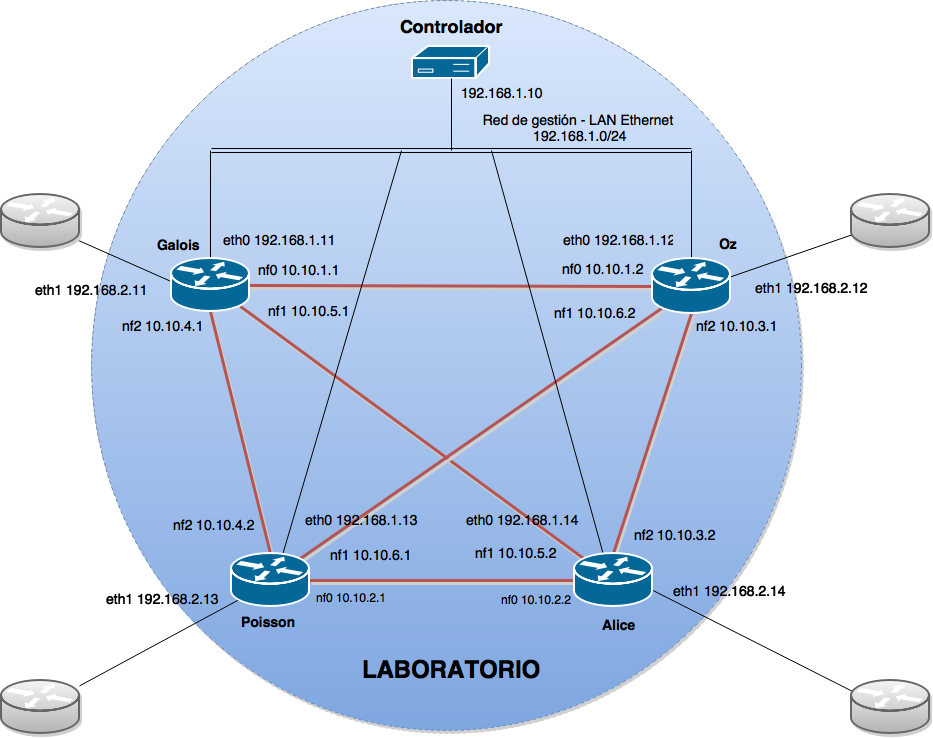
\includegraphics[width=0.85\textwidth]{Topologia}
\caption[Laboratorio de pruebas - Topolog\'ia]{Laboratorio de pruebas - Topolog\'ia}
\label{fig:LaboratorioDePruebasTopo}
\end{figure}

El laboratorio se compone de cuatro nodos implementados en base al dispositivo RAU-Switch conectados entre si con enlaces de fibra \'optica multimodo. Cada nodo esta conectado a los otros tres nodos de la topolog\'ia implementando de esta forma una topolog\'ia full mesh de cuatro nodos.

A su vez cada nodo esta conectado al controlador SDN del prototipo mediante una interfaz de red de 10Mb (interfaces \textbf{eth0}).\\

Por la forma que tiene la topolog\'ia, los cuatro nodos nombrados \textit{Galois}, \textit{Poisson}, \textit{Oz} y \textit{Alice} son nodos de borde. Esto quiere decir que RAUFlow los considera como nodos habilitados para ser nodo de ingreso \'o nodo de egreso en la definici\'on de servicios de redes privadas.

Por otro lado cada nodo cuenta con una interfaz de red de 100Mb (interfaz \textbf{eth1}) utilizada como interfaz externa para la conexi\'on con otras subredes. Estas interfaces son utilizadas por RAUFlow para la definici\'on de servicios de VPN como los puntos de entrada y salida de tr\'afico. Por tanto cada una de estas interfaces se encuentra directamente conectada a la subred de una VPN en particular.\\  

Como se menciona anteriormente en lacp\'itulo 5, la representaci\'on utilizada para modelar una topolog\'ia de red es la de un multigrafo dirigido ponderado. En la figura \ref{fig:LaboratorioDePruebasCostos} se muestra esta representaci\'on para la topolog\'ia del prototipo. Como puede apreciarse en la im\'agen cada enlace tiene su respectivo costo asociado.

Por simplicidad en el diagrama se han obviado los enlaces existentes entre el Controlador y cada uno de los nodos. Como se menciona en el cap\'itulo 4 la instancia de Quagga ejecutada en el controlador tiene como \'unico objetivo contar con un acceso local a la LSDB. Por ello conceptualmente el costo asociado a cada uno de estos enlaces es infinito, lo cual en pr\'actica se realiza asignando el valor 65535.  

\begin{figure}[ht!] 
\centering    
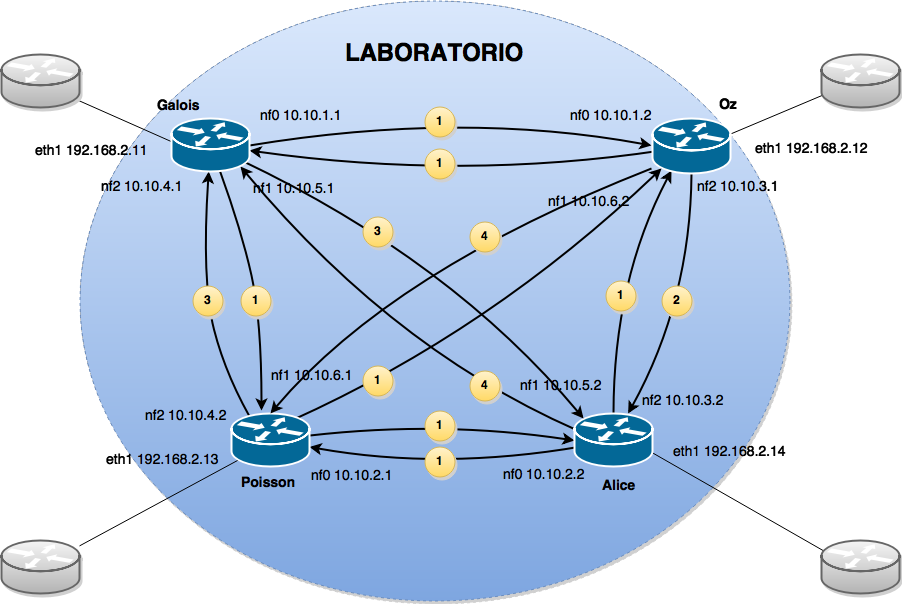
\includegraphics[width=0.85\textwidth]{TopologiaCostos}
\caption[Laboratorio de pruebas - Costos de la topolog\'ia]{Laboratorio de pruebas - Costos de la topolog\'ia}
\label{fig:LaboratorioDePruebasCostos}
\end{figure}

Sobre este laboratorio se implementan dos casos de uso representativos: (a) VPN de capa 3 y (b) VPN de capa 2. Sobre cada uno de estos casos de uso a su vez se ejecutan una serie de pruebas orientadas a verificar el correcto funcionamiento de las componentes m\'as importantes en la implementaci\'on de RAUFlow y RAU-Switch.

A continuaci\'on se describen los resultados obtenidos en la implementaci\'on de estos casos de uso y la ejecuci\'on de estas pruebas, comenzando por el caso de uso VPN de capa 3.

\section{VPN de capa 3}

Las redes privadas virtuales de capa 3 son un tipo de servicio comunmente brindado por un operador de red y es en particular uno de los servicios que se quiere implementar en la RAU2. En particular sobre este tipo de redes privadas puede implementarse clasificaci\'on de tr\'afico por tipo de aplicaci\'on o numeraci\'on de capa 3 por ejemplo.\\

En este trabajo se implementan dos escenarios diferentes para este tipo de red privada: (a) red privada multipunto con una \'unica organizaci\'on y tres sucursales f\'isicamente separadas, (b) red privada punto a punto con dos organizaciones, cada una de ellas con dos sucursales f\'isicamente separadas.

A continuaci\'on se detalla la construcci\'on de ambos escenarios y los resultados obtenidos.

\subsection{Escenario 1 - Red Privada Multipunto}

Este escenario representa una red privada multipunto de capa 3. En el mismo se tiene una sola organizaci\'on o red privada dividida en 3 sucursales o subredes físicamente separadas.

\begin{figure}[ht!] 
\centering    
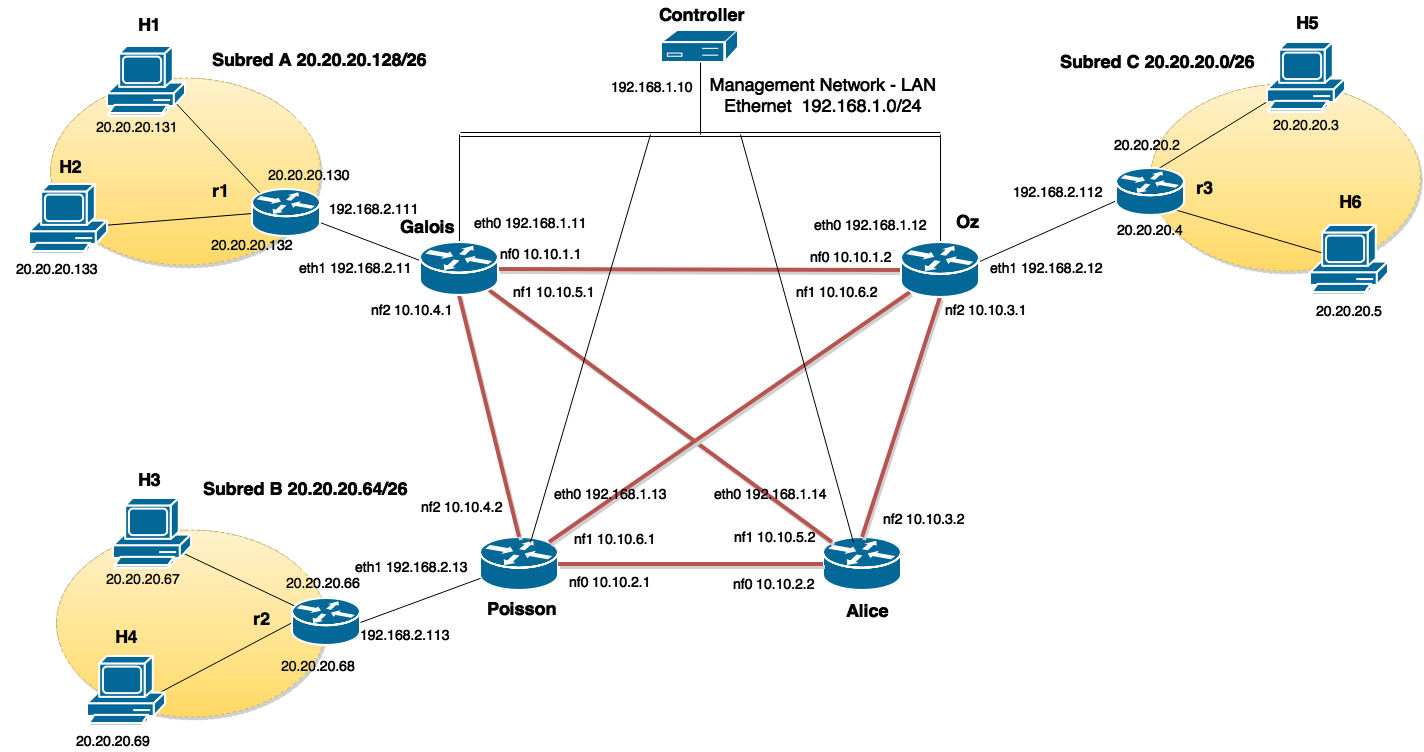
\includegraphics[width=1.0\textwidth]{CU1P1}
\caption[VPN de capa 3 - Escenario 1]{VPN de capa 3 - Escenario 1}
\label{fig:CUP1}
\end{figure}

Sobre este escenario se ejecutan una serie de pruebas orientadas a verificar los siguientes aspectos relacionados al prototipo:

\begin{enumerate}
\item Algoritmo de ruteo
\item Algoritmo de distribución de etiquetas
\item Clasificaci\'on de tr\'afico
\item Actualizaci\'on de rutas cuando cambia la topolog\'ia
\item Capacidad para crear VPN multipunto
\end{enumerate}

Para construir la red privada multipunto uniendo las tres subredes mencionadas y adem\'as verificar los puntos anteriores, se instancian los siguientes servicios(ver tabla \ref{table:TablaFlujos}). Por cada par de subredes se crean dos servicios (un servicio para cada sentido del tr\'afico).\\

\begin{table}[h]
\begin{tabular}{| l | l | l | p{4cm} | p{4cm} |}
\hline
Nombre & Ingreso & Egreso & Clasificación & Descripción \\ \hline

\crule[Aquamarine]{0.3cm}{0.3cm} S1 & Galois - eth1 & Oz - eth1 & ip\_src=20.20.20.128/26 ip\_dst=20.20.20.0/26 eth\_type=0x0800 & Tr\'afico IP de Subred A a Subred C \\ \hline

\crule[Red]{0.3cm}{0.3cm} S2 & Oz - eth1 & Galois - eth1 & ip\_src=20.20.20.0/26 ip\_dst=20.20.20.128/26 eth\_type=0x0800 & Tr\'afico IP de Subred C a Subred A \\ \hline

\crule[ForestGreen]{0.3cm}{0.3cm} S3 & Galois - eth1 & Poisson - eth1 & ip\_src=20.20.20.128/26 ip\_dst=20.20.20.64/26 eth\_type=0x0800 & Tr\'afico IP de Subred A a Subred B \\ \hline

\crule[LimeGreen]{0.3cm}{0.3cm} S4 & Poisson - eth1 & Galois - eth1 & ip\_src=20.20.20.64/26 ip\_dst=20.20.20.128/26 eth\_type=0x0800 & Tr\'afico IP de Subred B a Subred A \\ \hline

\crule[RoyalPurple]{0.3cm}{0.3cm} S5 & Poisson - eth1 & Oz - eth1 & ip\_src=20.20.20.64/26 ip\_dst=20.20.20.0/26 eth\_type=0x0800 IP & Tr\'afico de Subred B a Subred C \\ \hline

\crule[YellowOrange]{0.3cm}{0.3cm} S6 & Oz - eth1 & Poisson - eth1 & ip\_src=20.20.20.0/26 ip\_dst=20.20.20.64/26 eth\_type=0x0800 & Tr\'afico IP de Subred C a Subred B \\ \hline 

\end{tabular}
\vspace{0.3cm}
\caption[CU1 - Escenario 1, servicios creados]{CU1 - Escenario 1, servicios creados}
\label{table:TablaFlujos}
\end{table}

Para cada uno de estos servicios adem\'as se indica el etherype 0x0800 correspondiente al tipo de tr\'afico IPv4.\\

Este conjunto de servicios establece el procesamiento de paquetes de capa 3 para las diferentes subredes de forma de conectarlas en una red privada de capa 3. Sin embargo no alcanzan para la implementaci\'on de la misma. Es necesario definir un conjunto de servicios adicionales.\\

Para fija ideas, cuando el host H1 en la sub red A envia un paquete con destino al host H3 en la subred B, primero envía el paquete al gateway de la subred A (r1) el cual entiende que el paquete debe ser reenviado al router de borde de la red del prototipo al cual esta conectada la subred, en este caso Galois. No obstante en este paso r1 no conoce la dirección de capa de enlace (direcci\'on MAC) que debe colocarse al paquete para ser reenviado a Galois; por ello utilizando el protocolo ARP (Address Resolution Protocol) inicia una consulta ARP con la direcci\'on del siguiente paso, el router r2 (192.168.2.113).

Para que esta consulta ARP pueda atravesar la red del laboratorio, así como su respuesta y para todas las combinaciones de consultas ARP en el escenario planteado, se instancian los siguientes servicios (ver tabla \ref{table:TablaFlujos2}). 

\begin{table}[h]
\begin{tabular}{| l | l | l | p{4cm} | p{4cm} |}
\hline
 
S7 & Galois - eth1 & Oz - eth1 & arp\_tpa=192.168.2.112 eth\_type=0x0806 & Consultas ARP Subred A a Subred C \\ \hline

S8 & Oz - eth1 & Galois - eth1 & arp\_tpa=192.168.2.111 eth\_type=0x0806 & Consultas ARP Subred C a Subred A \\ \hline

S9 & Galois - eth1 & Poisson - eth1 & arp\_tpa=192.168.2.113 eth\_type=0x0806 & Consultas ARP Subred A a Subred B \\ \hline

S10 & Poisson - eth1 & Galois - eth1 & arp\_tpa=192.168.2.111 eth\_type=0x0806 & Consultas ARP Subred B a Subred A \\ \hline

S11 & Poisson - eth1 & Oz - eth1 & arp\_tpa=192.168.2.112 eth\_type=0x0806 & Consultas ARP Subred B a Subred C \\ \hline

S12 & Oz - eth1 & Poisson - eth1 & arp\_tpa=192.168.2.113 eth\_type=0x0806 & Consultas ARP Subred C a Subred B \\ \hline

\end{tabular}
\vspace{0.3cm}
\caption[CU1 - Escenario 1, servicios adicionales]{CU1 - Escenario 1, servicios adicionales}
\label{table:TablaFlujos2}
\end{table}

Ahora si, se tiene definido el conjunto de servicios que implementa la red privada de capa 3 multipunto en dicho escenario, utilizando el prototipo. A continuaci\'on se detallan las pruebas realizadas para cada uno de los aspectos mencionados anteriormente.

\subsubsection{Verificaci\'on de Algoritmo de ruteo}
En esta secci\'on se eval\'ua el correcto funcionamiento del algoritmo de ruteo. Para ello se comparan los caminos computados por el algoritmo para cada servicio, con los respectivos mejores caminos te\'oricos(previamente calculados de forma manual). 

Para cada camino se verifican dos cosas: (1) que el camino calculado se corresponde con el camino te\'orico y (2) que el camino es correctamente instalado en forma de reglas de reenvío (en base a conmutaci\'on de etiquetas) en las respectivas tablas de flujos OpenFlow de cada nodo en el camino.\\

Como se ha mencionado, los caminos te\'oricos son calculados manualmente observando los costos de la topolog\'ia (figura \ref{fig:LaboratorioDePruebasCostos}). Los resultados de este procedimiento se muestran en la figura \ref{fig:CUP1Caminos}. Cada camino es identificado mediante el código de color de cada servicio, omitiendo los servicios de la tabla \ref{table:TablaFlujos2} con el objetivo de simplificar el diagrama.\\

\begin{figure}[ht!] 
\centering    
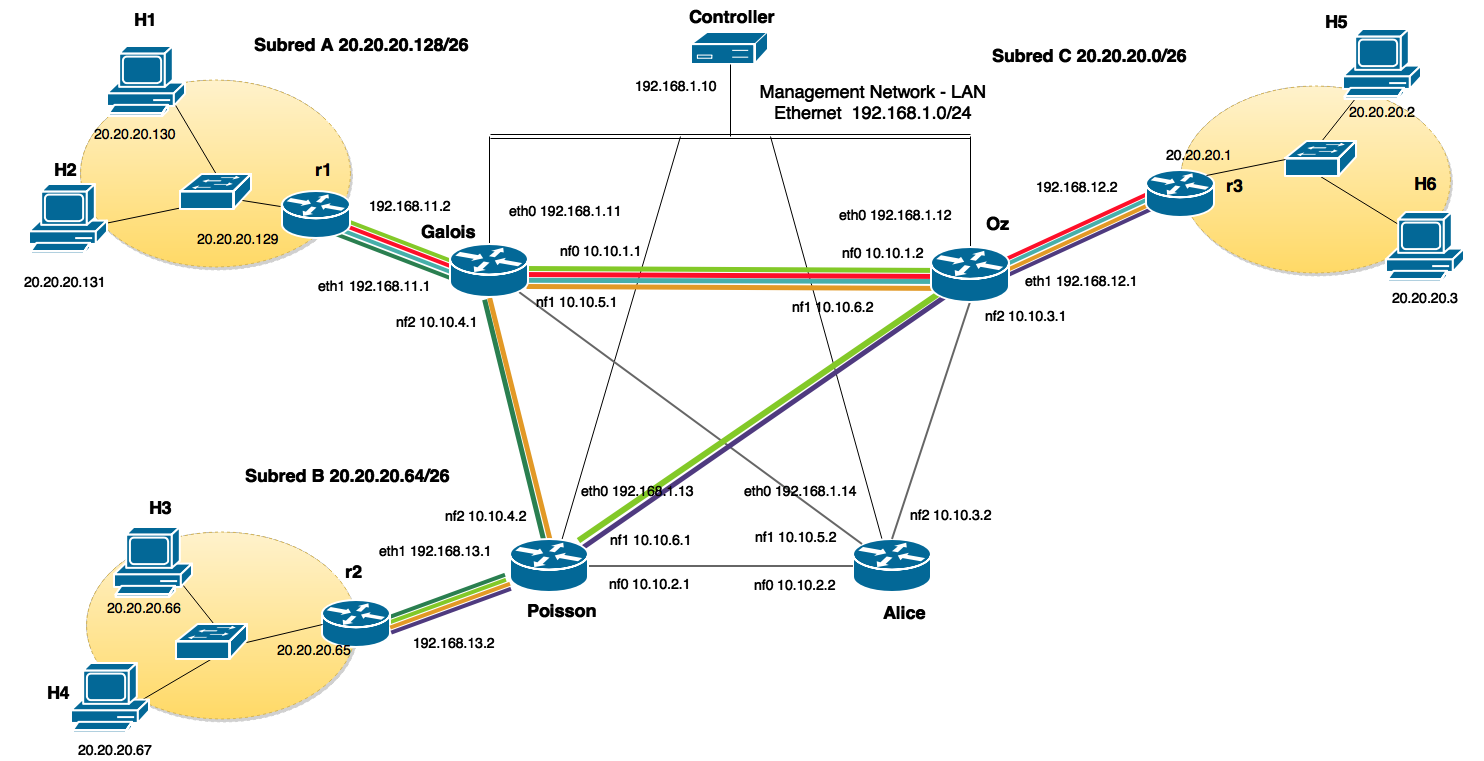
\includegraphics[width=1.0\textwidth]{CU1P1Caminos}
\caption[Escenario 1 - Caminos para servicios]{Escenario 1 - Caminos para servicios}
\label{fig:CUP1Caminos}
\end{figure}

Para obtener los caminos calculados por el algoritmo de ruteo, se analizan las tablas de flujos de Open vSwitch en cada nodo de la red del laboratorio. A partir del contenido de estas tablas fácilmente puede reconstruirse el camino previamente calculado.\\

En las figuras ~\ref{fig:CU1P1DumpFlows1}~-~\ref{fig:CU1P1DumpFlows4} se muestran las tablas de flujos asociadas a cada nodo del laboratorio. Para conseguir esta informaci\'on se utiliza el comando \textbf{dump-flows} de la herrmaienta Open vSwitch. Sin embargo puede obtenerse tambi\'en esta informaci\'on desde la propia interfaz gr\'afica de RAUFlow.\\

\newpage
\begin{figure}[ht!] 
\centering    
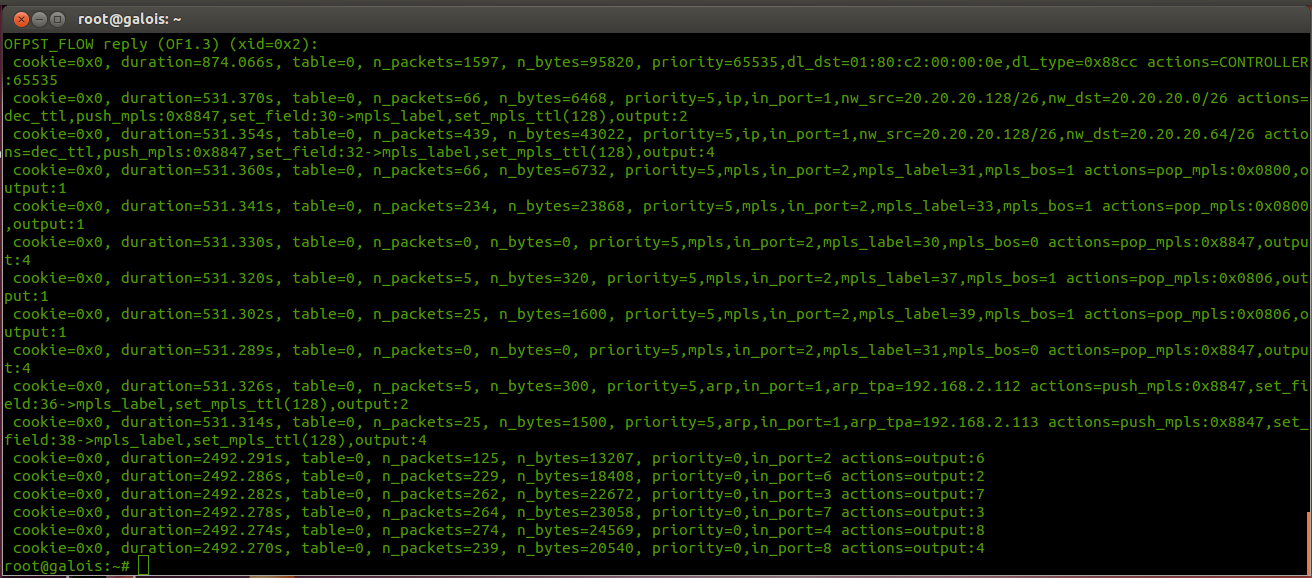
\includegraphics[width=1.0\textwidth]{LabE1P1Gal}
\caption[Tabla de flujos ovs - Galois]{Tabla de flujos ovs - Galois}
\label{fig:CU1P1DumpFlows1}
\end{figure}

\begin{figure}[h!] 
\centering    
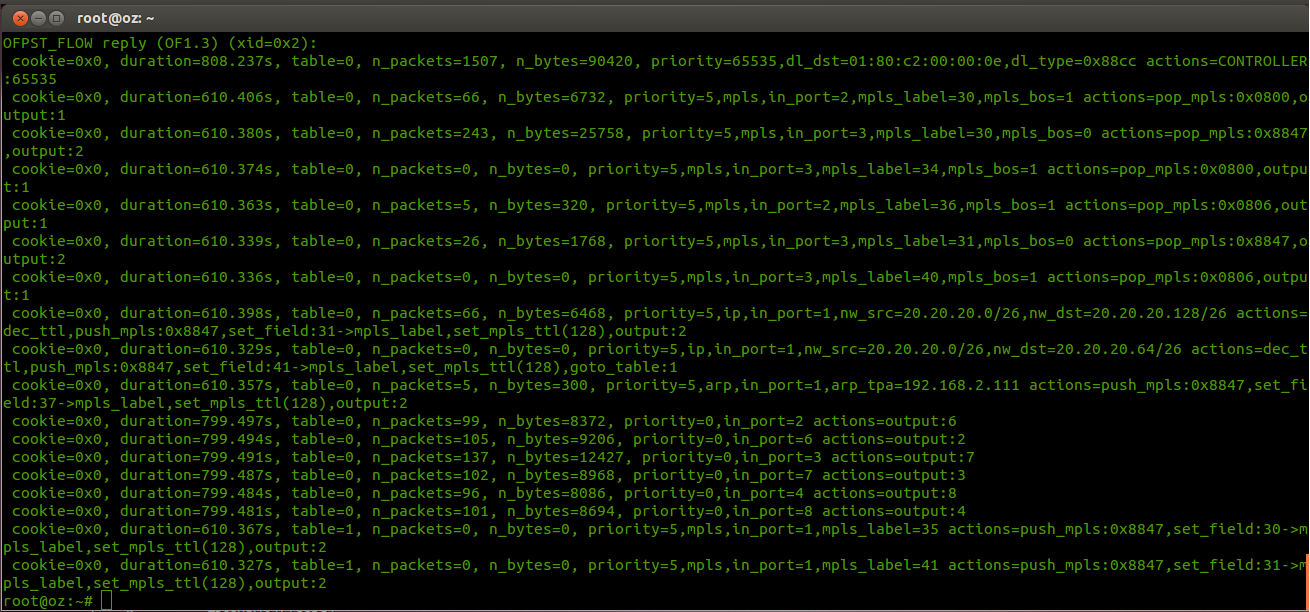
\includegraphics[width=1.0\textwidth]{LabE1P1Oz}
\caption[Tabla de flujos ovs - Oz]{Tabla de flujos ovs - Oz}
\label{fig:CU1P1DumpFlows2}
\end{figure}

\begin{figure}[h!] 
\centering    
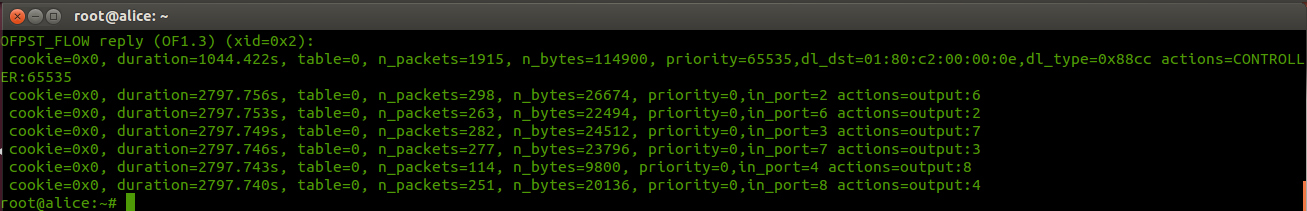
\includegraphics[width=1.0\textwidth]{LabE1P1Al}
\caption[Tabla de flujos ovs - Alice]{Tabla de flujos ovs - Alice}
\label{fig:CU1P1DumpFlows3}
\end{figure}

\begin{figure}[h!] 
\centering    
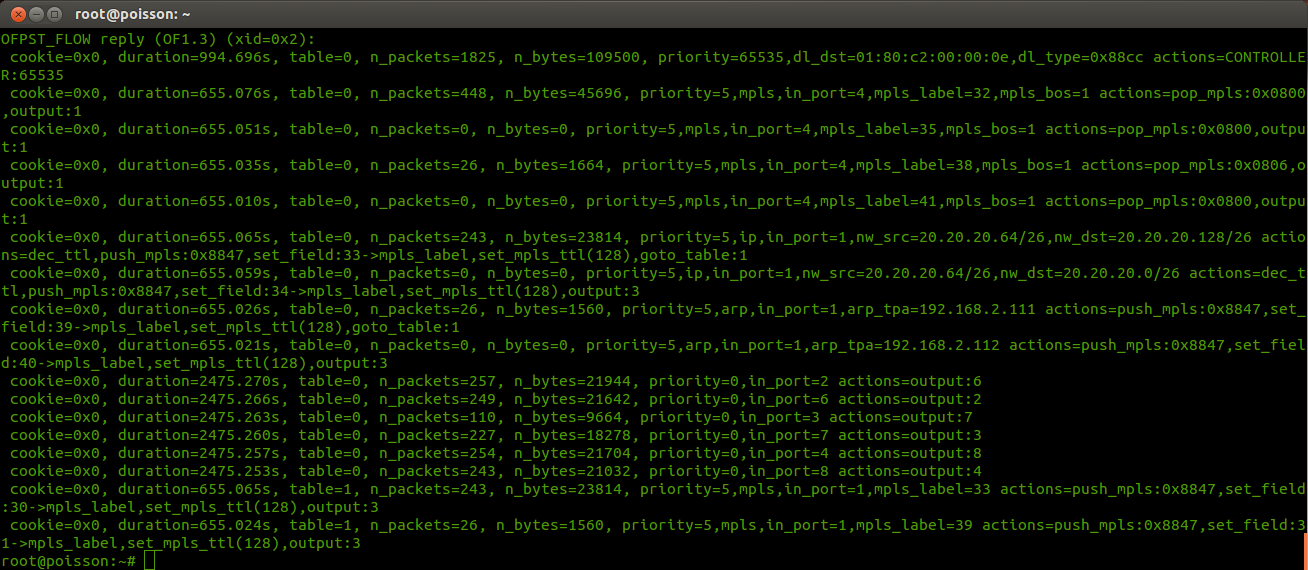
\includegraphics[width=1.0\textwidth]{LabE1P1Poi}
\caption[Tabla de flujos ovs - Poisson]{Tabla de flujos ovs - Poisson}
\label{fig:CU1P1DumpFlows4}
\end{figure}

\newpage
Asumiendose la notaci\'on $(n, i)$ para referirse a un enlace, donde \textit{n} indica nodo origen e \textit{i} interfaz de reenvío en \textit{n} para el próximo salto, entonces $<(n_1, i_1), \dots, (n_k, i_k)>$ puede usarse para denotar un camino en el laboratorio. De esta forma se pueden comparar f\'acilmente los caminos te\'oricos con los calculados.\\

Tomando como ejemplo el caso del servicio S3, el camino te\'orico puede denotarse de la siguiente forma:
 
$$<(Galois, nf_2)>$$

En otras palabras todo tr\'afico IP con origen en la subred A y destino a la subred B, es encaminado a través de la interfaz $nf_2$ en el nodo de ingreso \textit{Galois}. Luego en el nodo de egreso \textit{Poisson} es reenviado por la correspondiente interfaz del servicio.\\

Analizando las tablas de flujos de los nodos \textit{Galois} y \textit{Poisson}, puede comprobarse fácilmente la correspondencia entre el camino calculado y el camino te\'orico.

Por un lado en la tabla de flujos del nodo \textit{Galois} se tiene el siguiente flujo:

%Por un lado, acorde a la definci\'on del servicio, Galois debería reenviar todo tr\'afico de tipo \textbf{ip} que ingresa por la interfaz eth1(la cual se corresponde con el n\'umero de puerto openflow 1), con origen en la subred 20.20.20.64/26 y destino 20.20.20.0/64 por la interfaz nf1(la cual se corresponde con el n\'umero de puerto openflow 3).

\begin{figure}[h]
\textit{cookie=0.0, duration=531.354s, table=0, n\_packets=0, n\_bytes=0, priority=5, \\
ip,in\_port=1, nw\_src=20.20.20.128/26,nw\_dst=20.20.20.0/26 \\
actions=dec\_ttl,push\_mpls:0x8847,set\_field:30->mpls\_label,set\_mpls\_ttl(128),output:4}
\centering
\caption{Flujo 1}
\label{fig:Flujo1}
\end{figure}

Este flujo toma todo paquete recibido por el puerto openflow identificado con el n\'umero 1(interfaz eth1), numeración IP origen 20.20.20.128/26(subred A) y destino 20.20.20.64/26 (subred B), decrementa el TTL del paquete, coloca un cabezal mpls con la etiqueta 32 y finalmente lo reenvía por el puerto openflow identificado con el n\'umero 4(interfaz nf2). Observar que el valor de la etiqueta mpls colocado es el utilizado para identificar el servicio(etiqueta interna). \\

%Notese adem\'as la acci\'on \textbf{dec\_ttl} en el flujo. Esta acci\'on es utilizada en cada nodo de borde en la definici\'on de un servicio para decrementar el ttl de un paquete ip cada vez que ingresa a la red del prototipo (en este caso a la red del laboratorio). Observese tambi\'en el valor de la etiqueta mpls(34) colocado en el paquete para identificar el servicio(etiqueta interna).

El procesamiento de los paquetes asociados al servicio S3 en el nodo \textit{Poisson}, esta dado por el siguiente flujo:

\begin{figure}[h]
\textit{cookie=0.0, duration=655.076s, table=0, n\_packets=0, n\_bytes=0, priority=5, \\
mpls,in\_port=4,mpls\_label=32,mpls\_bos=1 \\
actions=pop\_mpls:0x0800,output:1 }
\centering
\caption{Flujo 2}
\label{fig:Flujo2}
\end{figure}

Este flujo toma todo paquete recibido por el puerto openflow n\'umero 4(interfaz nf2), retira el cabezal mpls y finalmente lo reenvía por el puerto n\'umero 1(interfaz eth1).\\

De esta forma todos los paquetes asociados al servicio S3 son transportados desde el nodo de ingreso \textit{Galois} al nodo de egreso \textit{Poisson} mediante un solo enlace, utilizando un solo nivel de etiquetas mpls.\\

Analizando el camino que deben seguir los paquetes que atraviesan la red del laboratorio en el sentido inverso; es decir, desde la subred B hacia la subred A(servicio S4), el camino teórico es el siguiente:

$$<(Poisson, nf_1), (Oz, nf_0)>$$ 

Analizando primero la tabla de flujos del nodo \textit{Poisson}, el primer salto del camino es implementado por los siguientes flujos:

\begin{center}
\textit{cookie=0.0, duration=655.065s, table=0, n\_packets=0, n\_bytes=0, priority=5, \\
ip,in\_port=1, nw\_src=20.20.20.64/26,nw\_dst=20.20.20.128/26 \\
actions=dec\_ttl,push\_mpls:0x8847,set\_field:33->mpls\_label,set\_mpls\_ttl(128), goto\_table:1 \\
cookie=0.0, duration=655.065s, table=0, n\_packets=0, n\_bytes=0, priority=5, \\
mpls,in\_port=1,mpls\_label=33 actions=push\_mpls:0x8847,set\_fied:30->mpls\_label,set\_mpls\_ttl(128),output:3
}
\end{center}

Notar como primera diferencia en comparación al camino anterior, en este caso se tienen dos flujos: un primer flujo para colocar la etiqueta asociada al servicio (etiqueta interna) y un segundo flujo para colocar la etiqueta de reenvío (etiqueta externa). 

El camino anterior carece de etiqueta externa puesto que al ser un camino de un solo salto, el primer nodo coincide con el pen\'ultimo, y al implementar PHP no es necesario colocar etiqueta externa. 

Tras colocar el par de etiquetas mpls sobre el paquete al ingreso, el mismo es reenviado a trav\'es del puerto n\'umero 3(interfaz nf1).\\

El siguiente salto en el camino, es implementado por el siguiente flujo en la tabla del nodo \textit{Oz}:

\begin{center}
\textit{cookie=0.0, duration=610.380s, table=0, n\_packets=243, n\_bytes=25748, priority=5, \\
mpls,in\_port=3,mpls\_label=30,mpls\_bos=0 actions=pop\_mpls:0x8847,output:2 }
\end{center}

Tras ingresar un paquete, se cambia el valor de la etiqueta externa para luego reenviarse por el puerto n\'umero 4(interfaz nf2).\\

Luego el tramo final del camino es implementado en el nodo \textit{Galois} mediante el siguiente flujo:

\begin{center}
\textit{cookie=0.0, duration=531.341s, table=0, n\_packets=234, n\_bytes=23868, priority=5, \\
mpls,in\_port=2,mpls\_label=33,mpls\_bos=1 actions=pop\_mpls:0x0800,output:1 }
\end{center}

Análogamente el lector puede completar el análisis de la correspondencia entre los caminos te\'oricos y los calculados por el algoritmo de ruteo. A continuaci\'on se analiza el algoritmo de distribucion de etiquetas.

\subsubsection{Verificaci\'on de Algoritmo de distribución de etiquetas}

[De repente comentar en funcion al escenario anterior porque anda bien]

En la siguiente secci\'on se analiza la clasificaci\'on de tr\'afico.

\subsubsection{Clasificaci\'on de tr\'afico}
Se implementa clasificaci\'on de tr\'afico en el nodo ingreso para un servicio en particular. En el escenario definido, se realiza clasificaci\'on de tr\'afico basándose en la numeraci\'on IP origen y destino de un paquete. De esta forma, por ejemplo el nodo Galois determina que camino debe tomar un paquete con origen en la Subred A y destino la Subred B. Luego en cada nodo intermedio los paquetes son procesados acorde a las reglas de reenvío en base a la conmutación de etiquetas mpls.

Para verificar el correcto funcionamiento de cada flujo OpenFlow involucrado en la clasificaci\'on de tr\'afico, as\'i como el posterior procesamiento dentro de la red del prototipo, se elige un servicio y se observa el procesamiento de los paquetes asociados en cada nodo involucrado en el camino.\\

\begin{figure}[ht!] 
\centering    
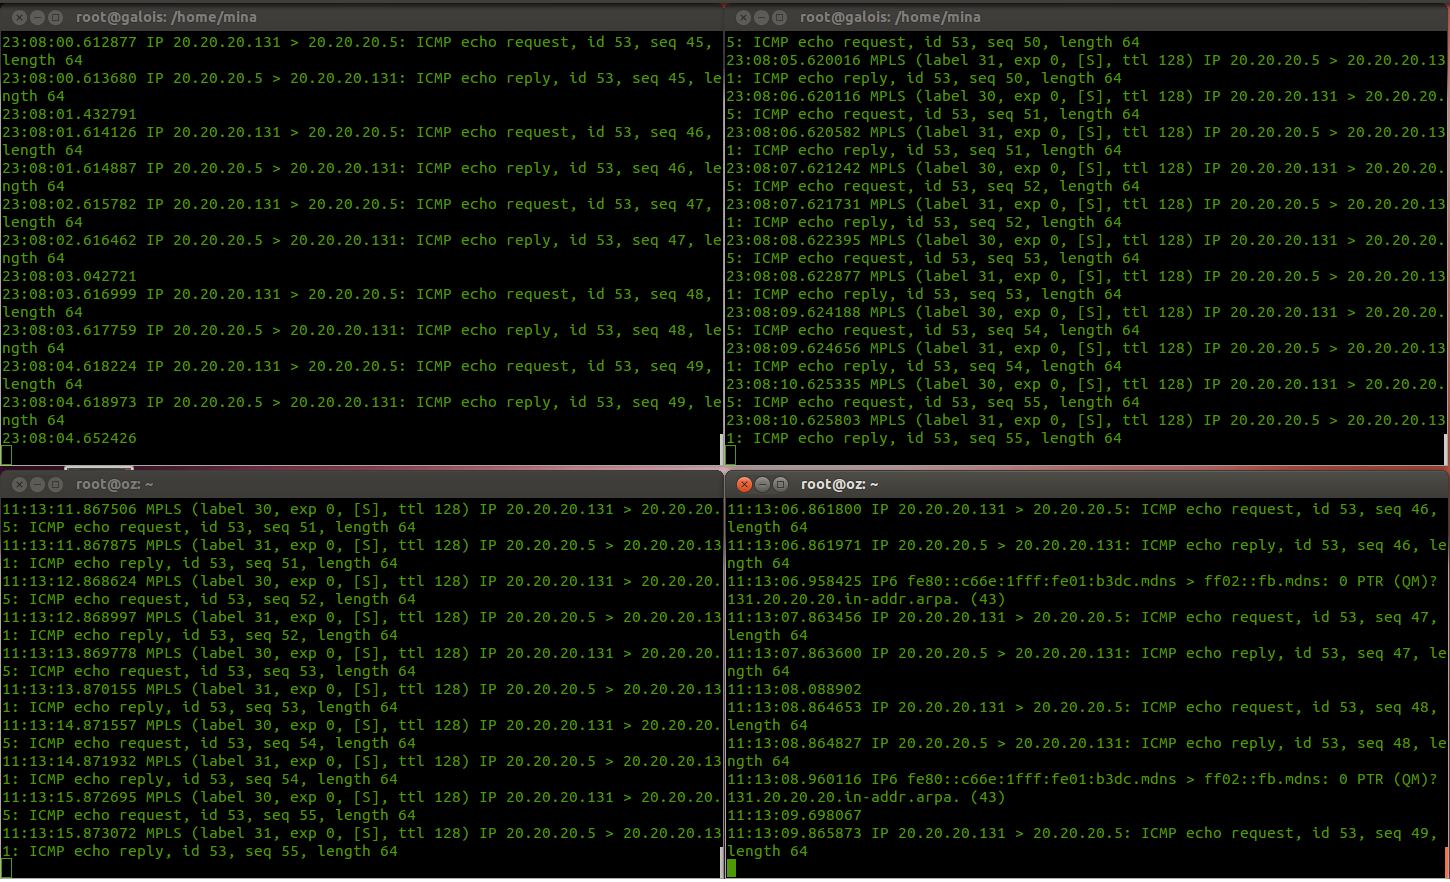
\includegraphics[width=1.0\textwidth]{LabE1P1CaputrasTrafico0}
\caption[Capturas de tr\'afico con tcpdump - servicio S1]{Capturas de tr\'afico con tcpdump - servicio S1}
\label{fig:LabE1P1CapsTraf}
\end{figure}

En la figura \ref{fig:LabE1P1CapsTraf} se muestra el procesamiento de los paquetes asociados al servicio S1 en cada uno de los nodos que componen al LSP, generando tr\'afico desde un host en la sub red A con destino a otro host en la subred C.

Como puede observarse en el primer cuarto de la imagen (cuarto superior izquierdo), el cual se corresponde con una captura hecha con el comando \textbf{tcpdump} en la interfaz \textbf{eth1} del nodo \textit{Galois}, se reciben paquetes ICMP request con origen 20.20.20.131 y destino 20.20.20.05. Tambi\'en puede observarse en esta imagen paquetes ICMP reply a los paquetes request enviados.

Luego, como se muestra en el segundo cuarto de la imagen(cuarto superior derecho), el cual se corresponde con una captura realizada en la interfaz nf0 de dicho nodo, a cada paquete ICMP request recibido por la interfaz eth1 se le coloca un cabezal mpls con la etiqueta 31 y se reenvía por la interfaz en cuestión. Finalmente al arribar al nodo \textit{Oz} por la interfaz \textbf{nf0} (cuarto inferior izquierdo de la imagen), el cabezal mpls es retirado de cada paquete para luego ser reenviado por la interfaz \textbf{eth1} hacia la subred C (cuarto inferior derecho de la imagen).\\

En la figura \ref{fig:LabE1P1CapHost} se muestra una captura de pantalla del comando ping utilizado para generar tr\'afico ICMP desde el host 20.20.20.131 en la subred A, al host 20.20.20.05 en la subred C.

\begin{figure}[h!] 
\centering    
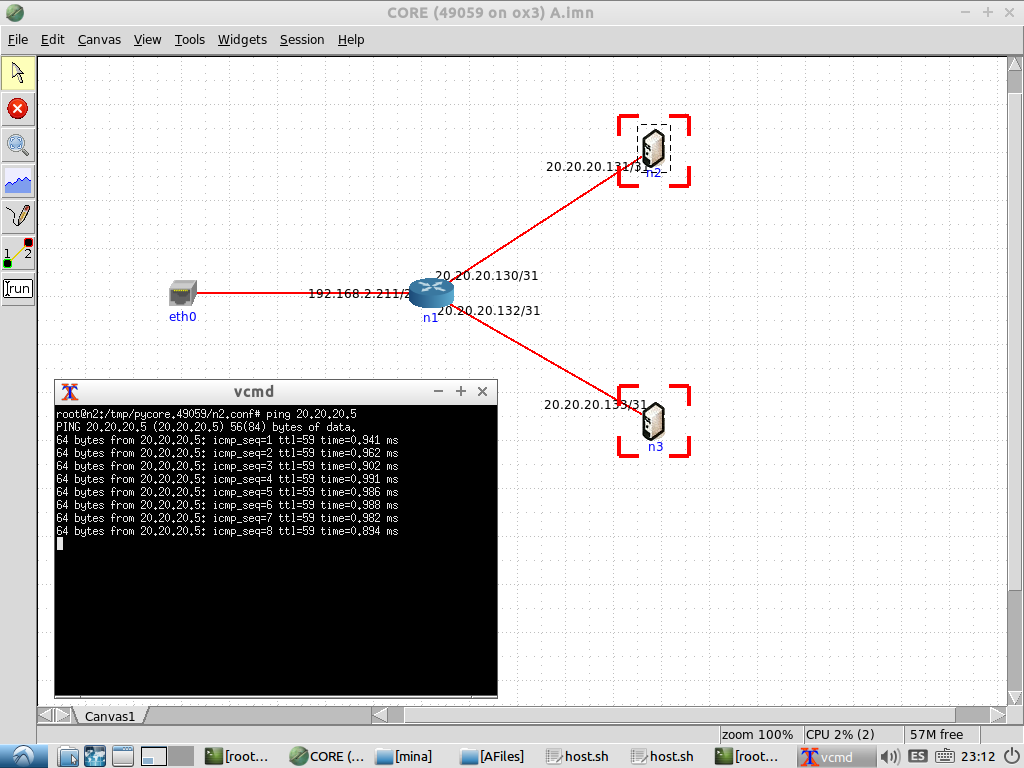
\includegraphics[width=0.6\textwidth]{E1P1202020131-2020205}
\caption[Capturas de comando ping H1-Subred A]{Capturas de comando ping H1-Subred A}
\label{fig:LabE1P1CapHost}
\end{figure}

Análogamente se procesan los paquetes asociados a los restantes servicios en el sistema. Para complementar el ejemplo anterior, en la figura \ref{fig:LabE1P1CapsTraf2} se muestra el procesamiento de los paquetes asociados al servicio S3, utilizando el comando ping para generar tr\'afico desde el host 20.20.20.131 en la subred A, al host 20.20.20.67 en la subred B. En la imagen se muestran las capturas de tr\'afico utilizando el comando tcpdump para las interfaces eth1 (cuarto superior izquierdo de la imagen) y nf2 (cuarto superior derecho de la imagen) en el nodo Galois, y las interfaces nf2 (cuarto inferior izquierdo) y eth1 (cuarto inferior derecho) en el nodo Poisson.\\

En la siguiente secci\'on se discute el comportamiento del prototipo, cuando la topolog\'ia cambia por ejemplo por una falla t\'ecnica en un enlace, utilizando el escenario y los servicios definidos anteriormente.

\begin{figure}[ht!] 
\centering    
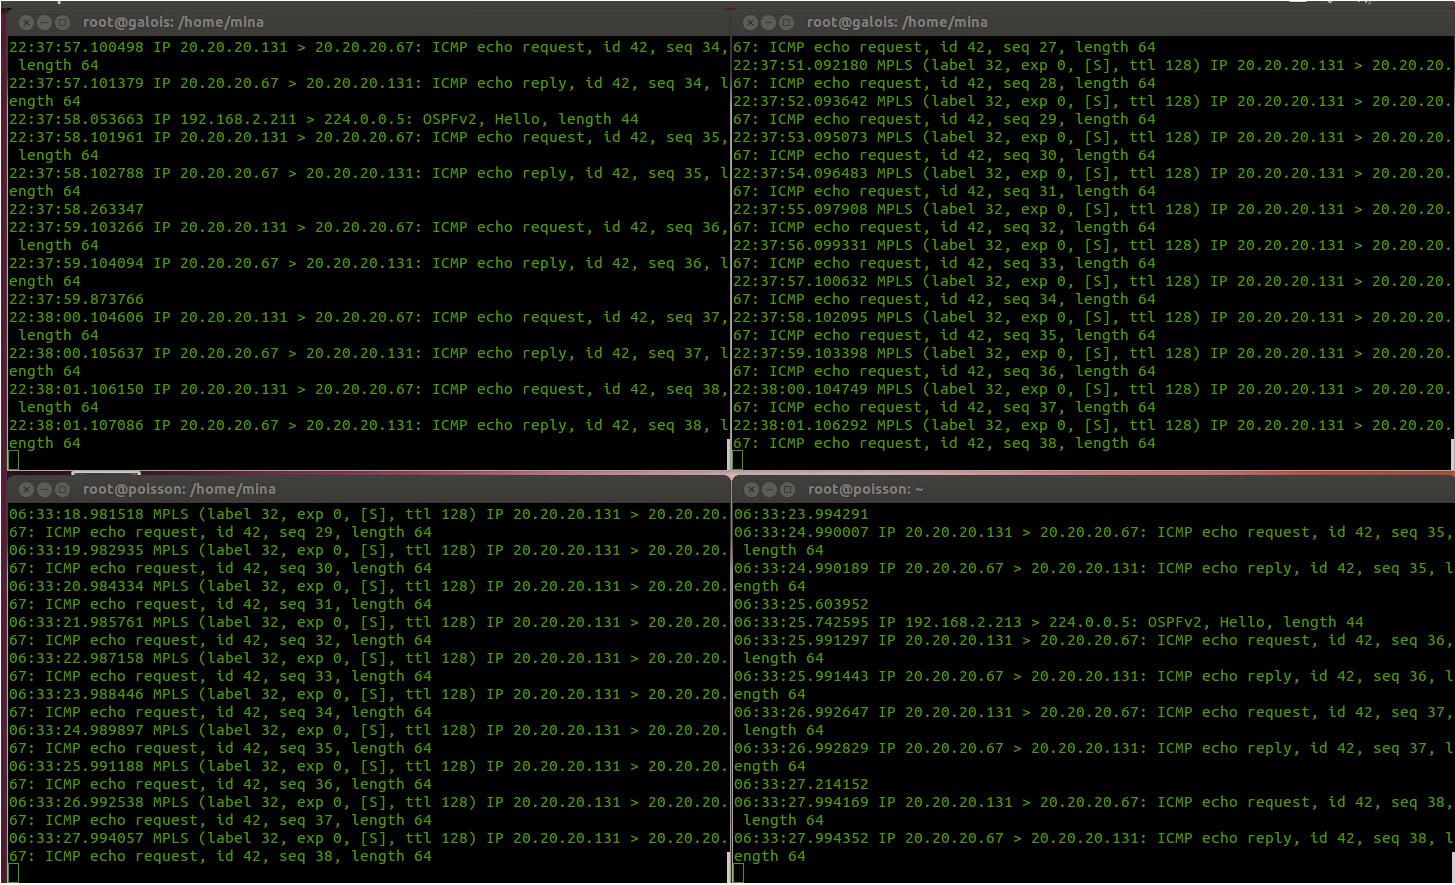
\includegraphics[width=1.0\textwidth]{LabE1P1CaputrasTrafico}
\caption[Capturas de tr\'afico con tcpdump - servicio S3]{Capturas de tr\'afico con tcpdump - servicio S3}
\label{fig:LabE1P1CapsTraf2}
\end{figure}

%Sin embargo RAUFlow admite realizar clasificaci\'on de tr\'afico por un conjunto bastante m\'as amplio de atributos. A continuaci\'on se definen una nueva lista de servicios orientados a demostrar la correcta implementaci\'on de esta funcionalidad.

%Cabe destacar que para esta prueba los servicios anteriormente creados son eliminados.

%\begin{table}[h]
%\begin{tabular}{| l | l | l | p{4cm} | p{4cm} |}
%\hline
%Nombre & Ingreso & Egreso & Clasificación & Descripción \\ \hline
%
%\crule[Aquamarine]{0.3cm}{0.3cm} S1 & Galois - eth1 & Oz - eth1 & ip\_src=20.20.20.128/26 ip\_dst=20.20.20.0/26 & Tr\'afico de Subred A a Subred C \\ \hline
%
%\crule[Red]{0.3cm}{0.3cm} S2 & Oz - eth1 & Galois - eth1 & ip\_src=20.20.20.0/26 ip\_dst=20.20.20.128/26 & Tr\'afico de Subred C a Subred A \\ \hline
%
%\crule[ForestGreen]{0.3cm}{0.3cm} S3 & Galois - eth1 & Poisson - eth1 & ip\_src=20.20.20.128/26 ip\_dst=20.20.20.64/26 & Tr\'afico de Subred A a Subred B \\ \hline
%
%\crule[LimeGreen]{0.3cm}{0.3cm} S4 & Poisson - eth1 & Galois - eth1 & ip\_src=20.20.20.64/26 ip\_dst=20.20.20.128/26 & Tr\'afico de Subred B a Subred A \\ \hline
%
%\crule[RoyalPurple]{0.3cm}{0.3cm} S5 & Poisson - eth1 & Oz - eth1 & ip\_src=20.20.20.64/26 ip\_dst=20.20.20.0/26 & Tr\'afico de Subred B a Subred C \\ \hline
%
%\crule[YellowOrange]{0.3cm}{0.3cm} S6 & Oz - eth1 & Poisson - eth1 & ip\_src=20.20.20.0/26 ip\_dst=20.20.20.64/26 & Tr\'afico de Subred C a Subred B \\ \hline
%\end{tabular}
%\vspace{0.3cm}

%\caption[CU1 - Escenario 1, servicios extra]{CU1 - Escenario 1, servicios extra}
%\label{table:TablaFlujos2}
%\end{table}

\newpage
\subsubsection{Actualizaci\'on de rutas}
Para probar el correcto funcionamiento del algoritmo de ruteo, en la actualizaci\'on de rutas existentes ante un cambio en la topolog\'ia, se trabaja con los servicios previamente definidos en \ref{table:TablaFlujos}.\\ 

Partiendo de este escenario, se simula un desperfecto t\'ecnico en los enlaces \\ $<(Galois, nf_2), (Poisson, nf_2)>$ y  $<(Poisson, nf_2), (Poisson, nf_2)>$ (por ejemplo simplemente desconectando el cable que conecta ambos nodos), provocando de esta forma una actualizaci\'on en la topolog\'ia y la posterior ejecuci\'on de los algoritmos de ruteo y distribución de etiquetas para los nuevos LSPs.\\ 
 
Acorde a los costos de la topolog\'ia (ver figura \ref{fig:LaboratorioDePruebasCostos}), en la nueva topolog\'ia los caminos te\'oricos asociados a cada servicio quedan de la siguiente forma:

\newpage
\begin{figure}[ht!] 
\centering    
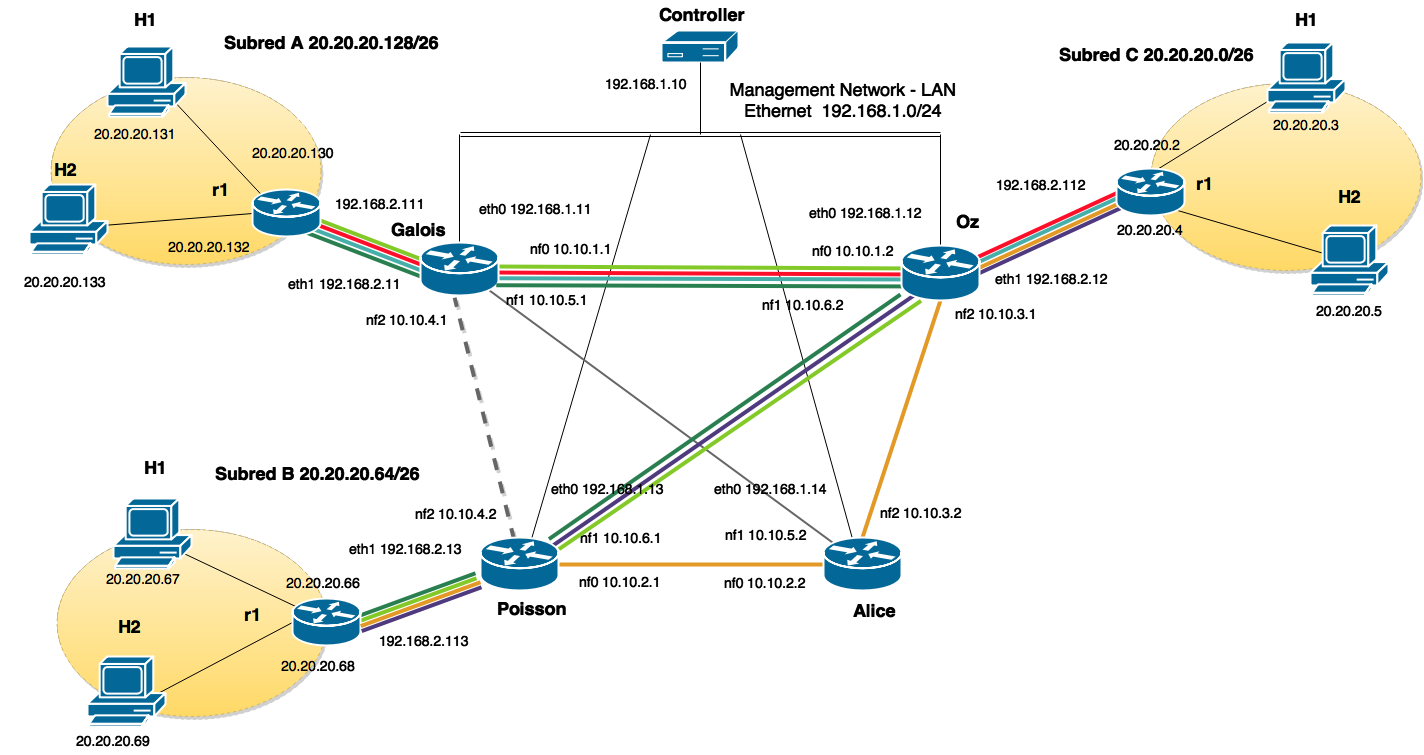
\includegraphics[width=1.0\textwidth]{CU1P1CaminosRecalculo}
\caption[Escenario 1 - Caminos para servicios recalculados]{Escenario 1 - Caminos para servicios recalculados}
\label{fig:CUP1Caminos2}
\end{figure}
 
Notese que los \'unicos caminos que cambian son los asociados a los servicios S3 y S6. Cabe destacar adem\'as que en la nueva topolog\'ia existe m\'as de un camino de m\'inimo costo para el servicio S3; los caminos $<(Galois, nf0), (Oz, nf1)>$ y $<(Galois, nf0), (Oz, nf2), (Alice, nf0)>$ presentan ambos el costo 4. Por tanto se tienen dos resultados v\'alidos posibles para la salida del algoritmo de ruteo para este servicio.\\

Para comprobar que el algoritmo de ruteo recaclula correctamente las rutas, se inspeccionan nuevamente las tablas de flujos de cada nodo en el laboratorio (ver figuras \ref{fig:CU1P2DumpFlows1}-\ref{fig:CU1P2DumpFlows4}), comparando los caminos calculados con los caminos te\'oricos.\\

\begin{figure}[h] 
\centering    
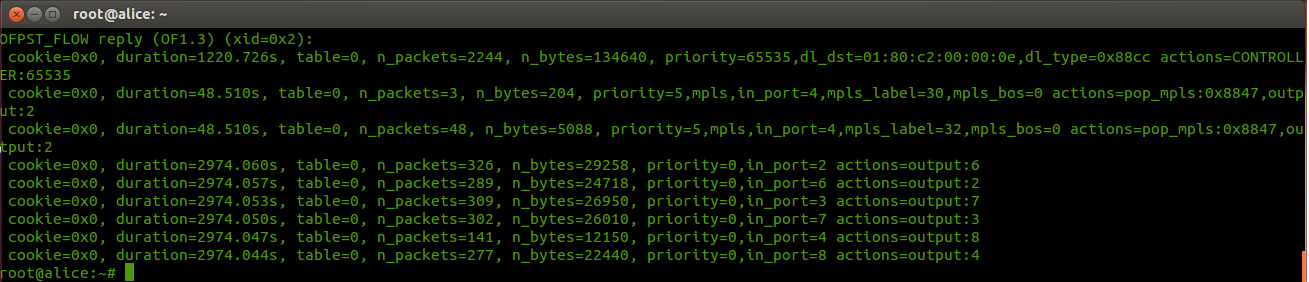
\includegraphics[width=1.0\textwidth]{LabE1P2Al}
\caption[Tabla de flujos ovs - Alice]{Tabla de flujos ovs - Alice}
\label{fig:CU1P2DumpFlows1}
\end{figure}

\newpage
\begin{figure}[h] 
\centering    
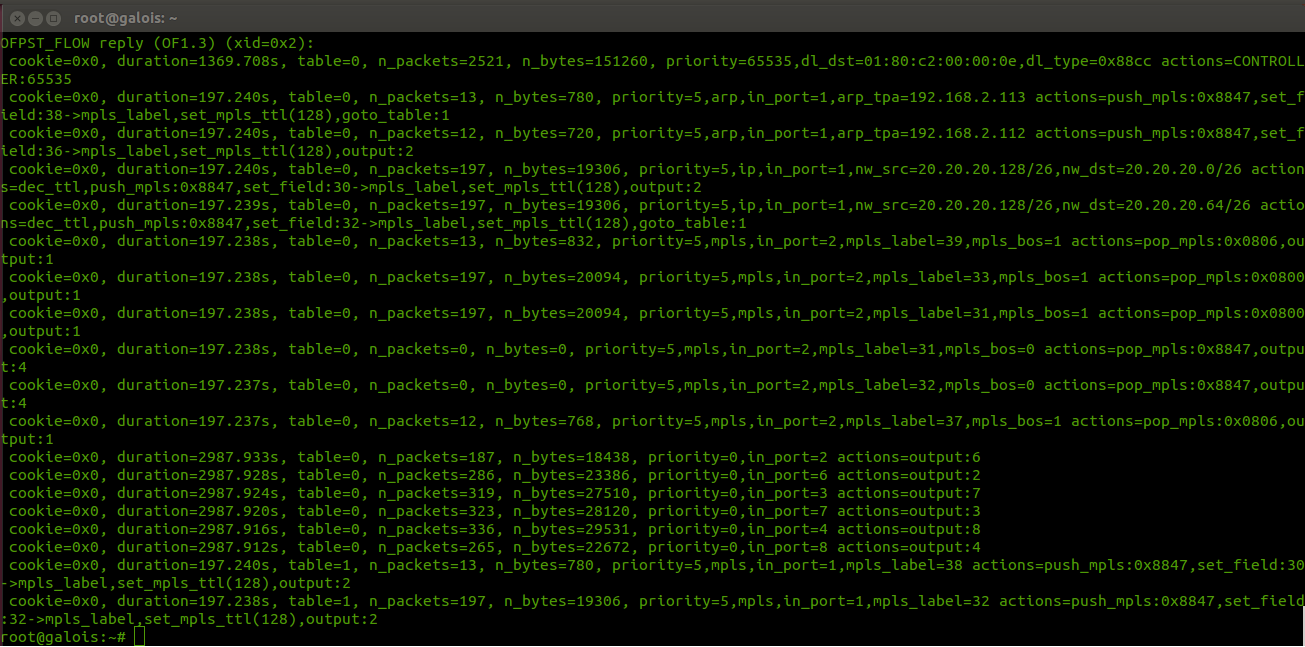
\includegraphics[width=1.0\textwidth]{LabE1P2Gal}
\caption[Tabla de flujos ovs - Galois]{Tabla de flujos ovs - Galois}
\label{fig:CU1P2DumpFlows2}
\end{figure}

\begin{figure}[h] 
\centering    
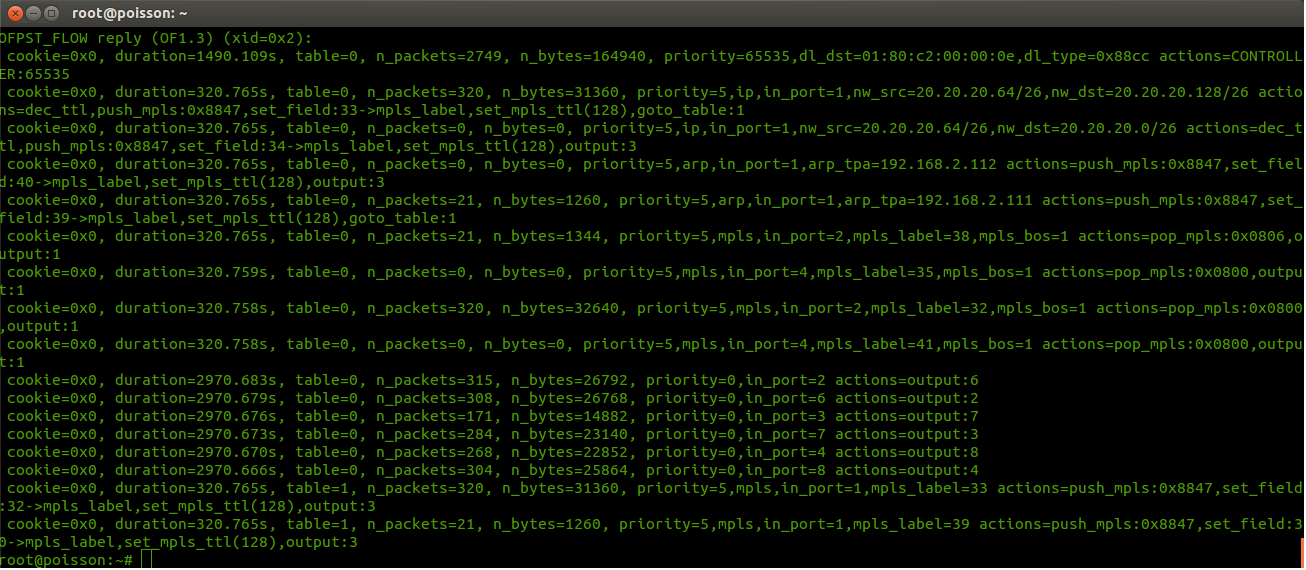
\includegraphics[width=1.0\textwidth]{LabE1P2Poi}
\caption[Tabla de flujos ovs - Poisson]{Tabla de flujos ovs - Poisson}
\label{fig:CU1P2DumpFlows3}
\end{figure}

\newpage
\begin{figure}[ht!] 
\centering    
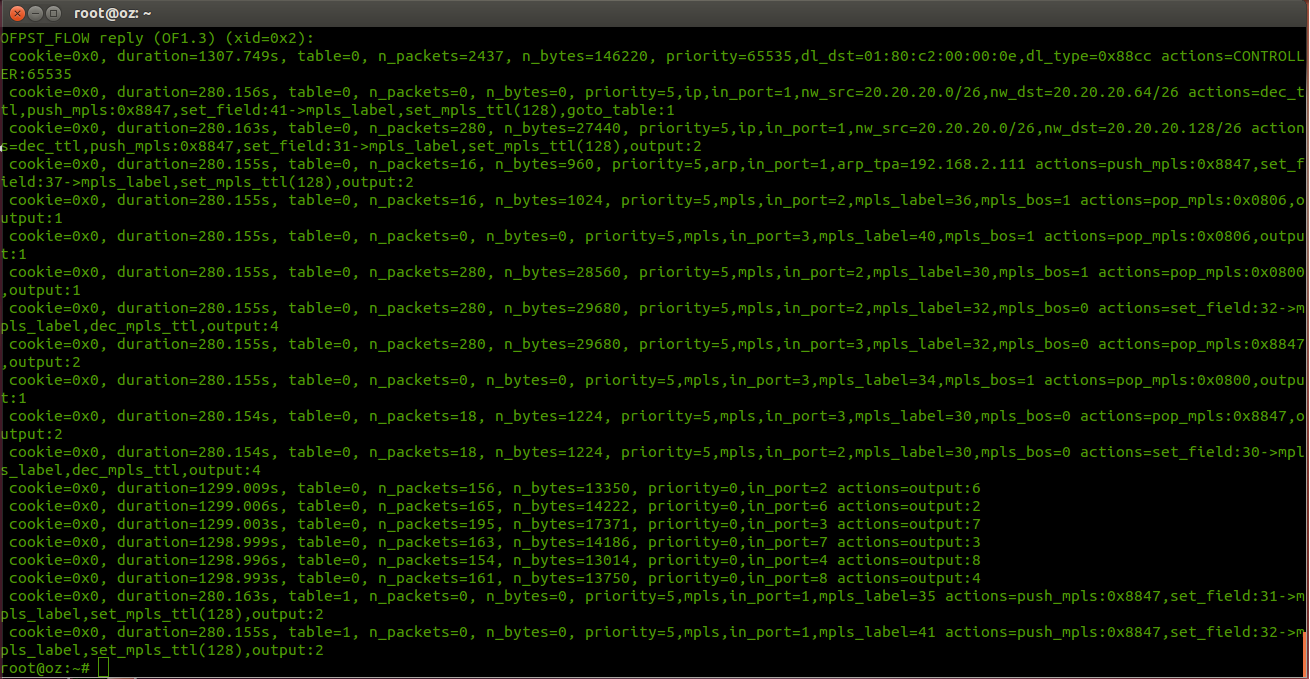
\includegraphics[width=1.0\textwidth]{LabE1P2Oz}
\caption[Tabla de flujos ovs - Oz]{Tabla de flujos ovs - Oz}
\label{fig:CU1P2DumpFlows4}
\end{figure}

Tomando como ejemplo la actualizaci\'on del LSP asociado al servicio S3, mientras que en la topolog\'ia original el camino asociado es $<(Galois, nf2)>$, tras la actualizaci\'on de la topolog\'ia el camino correcto puede ser o bien $<(Galois, nf0),(Oz, nf1)>$ o bien \\ $<(Galois, nf0), (Oz, nf2), (Alice, nf0)>$.\\

Al cambiar el camino, los flujos asociados a cada nodo en el camino tambi\'en deben cambiar. En particular como el camino nuevo no comparte ning\'un salto con el camino original, los flujos asociados al camino viejo deben ser eliminados de cada nodo.

Recordando la tabla de flujos original del nodo \textit{Galois} (ver imagen \ref{fig:CU1P1DumpFlows1}), el flujo \ref{fig:Flujo1} es utilizado para procesar y reenviar paquetes al nodo Poisson. En la tabla de flujos actualizada, este flujo es remplazado por el siguiente flujo (ver imagen \ref{fig:CU1P2DumpFlows2}):

\begin{center}
\textit{cookie=0.0, duration=192.239s, table=0, n\_packets=197, n\_bytes=19306, priority=5, \\
ip,in\_port=1, nw\_src=20.20.20.128/26,nw\_dst=20.20.20.64/26 \\
actions=dec\_ttl,push\_mpls:0x8847,set\_field:32->mpls\_label,set\_mpls\_ttl(128), goto\_table:1 \\
cookie=0.0, duration=197.238s, table=0, n\_packets=197, n\_bytes=19306, priority=5, \\
mpls,in\_port=1,mpls\_label=32 actions=push\_mpls:0x8847,set\_fied:32->mpls\_label,set\_mpls\_ttl(128),output:2}
\end{center}

Mediante este par de flujos, se les colocan dos cabezales mpls a los paquetes asociados al servicio, para luego ser reenviados por el puerto numero 2 (interfaz nf0) al nodo \textit{Oz}.\\

Por otra parte en la tabla de flujos del nodo \textit{Oz}, se incorpora el siguiente flujo:

\begin{center}
\textit{cookie=0.0, duration=280.155s, table=0, n\_packets=280, n\_bytes=29680, priority=5, \\
mpls,in\_port=2,mpls\_label=32,mpls\_bos=0 actions=set\_field:30->mpls\_label,dec\_mpls\_ttl,output:4 }
\end{center}

El mismo implementa el cambio de etiqueta mpls en el paquete, y su posterior reenvio por el puerto n\'umero 4 (interfaz nf2).\\

Luego en la tabla de flujos del nodo \textit{Alice} se incorpora el siguiente flujo:

\begin{center}
\textit{cookie=0.0, duration=48.510s, table=0, n\_packets=48, n\_bytes=5088, priority=5, \\
mpls,in\_port=2,mpls\_label=32,mpls\_bos=0 actions=pop\_mpls:0x8847,output:2 }
\end{center}

Este flujo implementa el pop de la etiqueta mpls externa en el penultimo nodo del LSP (penultimate-pop-hoping). Tras realizar esta acci\'on reenvia el paquete por el puerto n\'umero 2 (interfaz nf0).\\

Finalmente cuando el paquete arriba al nodo \textit{Poisson}, el procesamiento final del paquete, realizado con anterioridad por el flujo \ref{fig:Flujo2} ahora se realiza mediante el siguiente flujo: 

\begin{center}
\textit{cookie=0.0, duration=320.758s, table=0, n\_packets=320, n\_bytes=32740, priority=5, \\
mpls,in\_port=2,mpls\_label=32,mpls\_bos=1 actions=pop\_mpls:0x0800,output:1 }
\end{center}

Análogamente se puede estudiar la correspondencia entre el camino te\'orico y el camino calculado para el servicio S6.
 
\subsection{Escenario 2}

Este escenario representa una red privada punto a punto de capa 3. Esta compuesto por dos organizaciones diferentes, cada una de ellas con dos sucursales f\'isicamente separadas. Adicionalmente  ambas organizaciones utilizan la misma numeraci\'on IP en sus respectivas subredes.\\

\begin{figure}[h] 
\centering    
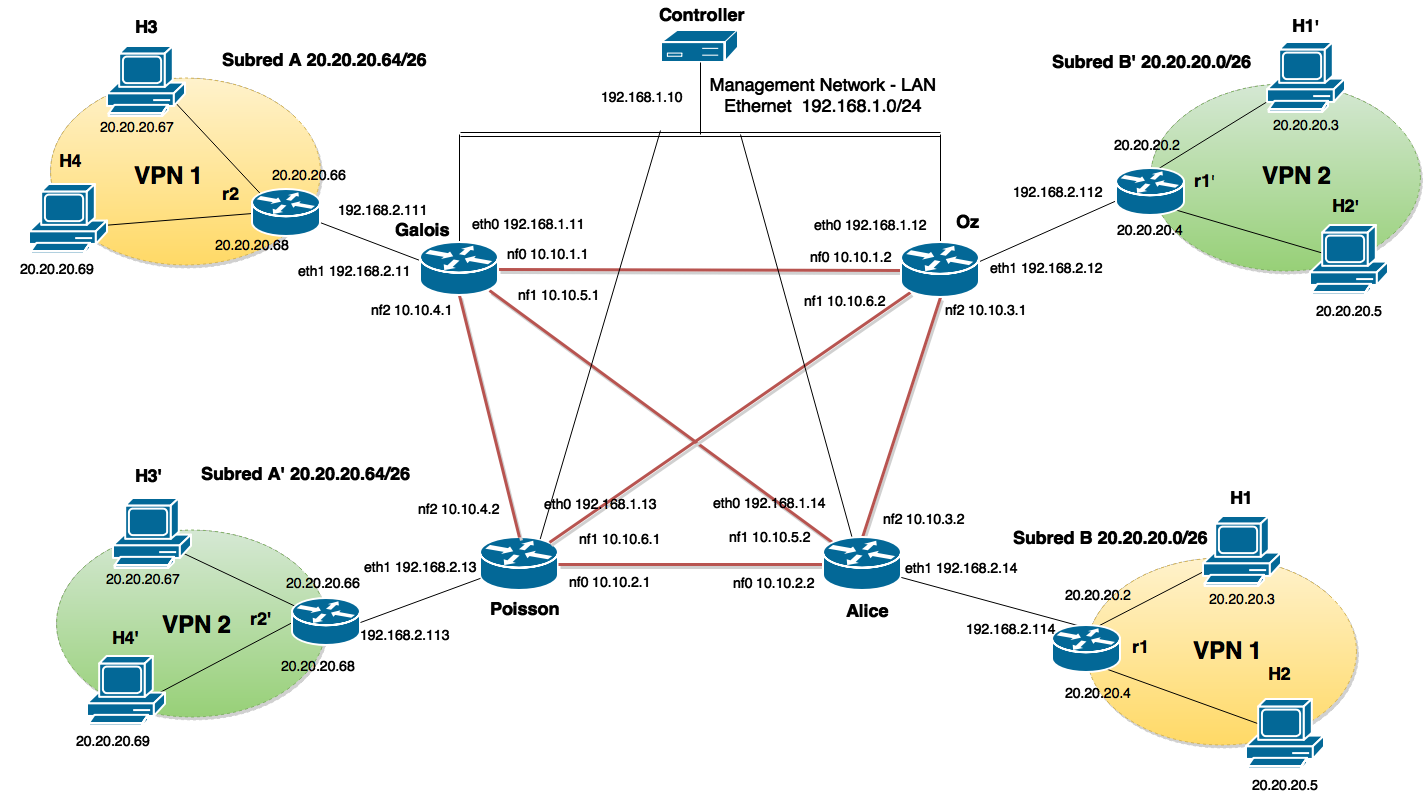
\includegraphics[width=1.0\textwidth]{CU1P2}
\caption[VPN de capa 3 - Escenario 2]{VPN de capa 3 - Escenario 2}
\label{fig:CUP2}
\end{figure}

Para la construcci\'on de este escenario se instancian los siguientes servicios en el sistema (ver tabla). Por cada red privada se instancian dos servicios (uno para cada sentido del tr\'afico).

\begin{table}[h]
\begin{tabular}{| l | l | l | p{4cm} | p{4cm} |}
\hline
Nombre & Ingreso & Egreso & Clasificación & Descripción \\ \hline

\crule[Aquamarine]{0.3cm}{0.3cm} S1 & Galois - eth1 & Alice - eth1 & ip\_src=20.20.20.64/26 ip\_dst=20.20.20.0/26 & Tr\'afico de Subred A a Subred B \\ \hline

\crule[Red]{0.3cm}{0.3cm} S2 & Alice - eth1 & Galois - eth1 & ip\_src=20.20.20.0/26 ip\_dst=20.20.20.64/26 & Tr\'afico de Subred B a Subred A \\ \hline

\crule[ForestGreen]{0.3cm}{0.3cm} S3 & Poisson - eth1 & Oz - eth1 & ip\_src=20.20.20.64/26 ip\_dst=20.20.20.0/26 & Tr\'afico de Subred A' a Subred B' \\ \hline

\crule[LimeGreen]{0.3cm}{0.3cm} S4 & Oz - eth1 & Poisson - eth1 & ip\_src=20.20.20.0/26 ip\_dst=20.20.20.64/26 & Tr\'afico de Subred B' a Subred A' \\ \hline

\end{tabular}
\vspace{0.3cm}
\caption[CU1 - Escenario 2]{CU1 - Escenario 2}
\label{table:TablaFlujos3}
\end{table}


\newpage
\begin{figure}[ht!] 
\centering    
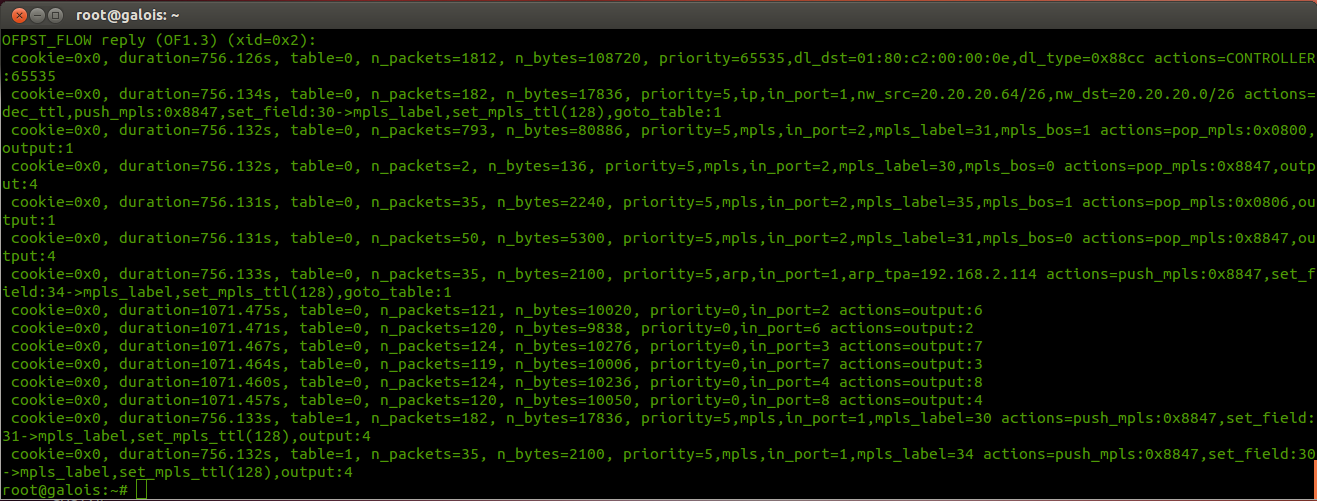
\includegraphics[width=1.0\textwidth]{E2P1Gal}
\caption[Tabla de flujos ovs - Galois]{Tabla de flujos ovs - Galois}
\label{fig:CU1P1DumpFlows1}
\end{figure}

\begin{figure}[h!] 
\centering    
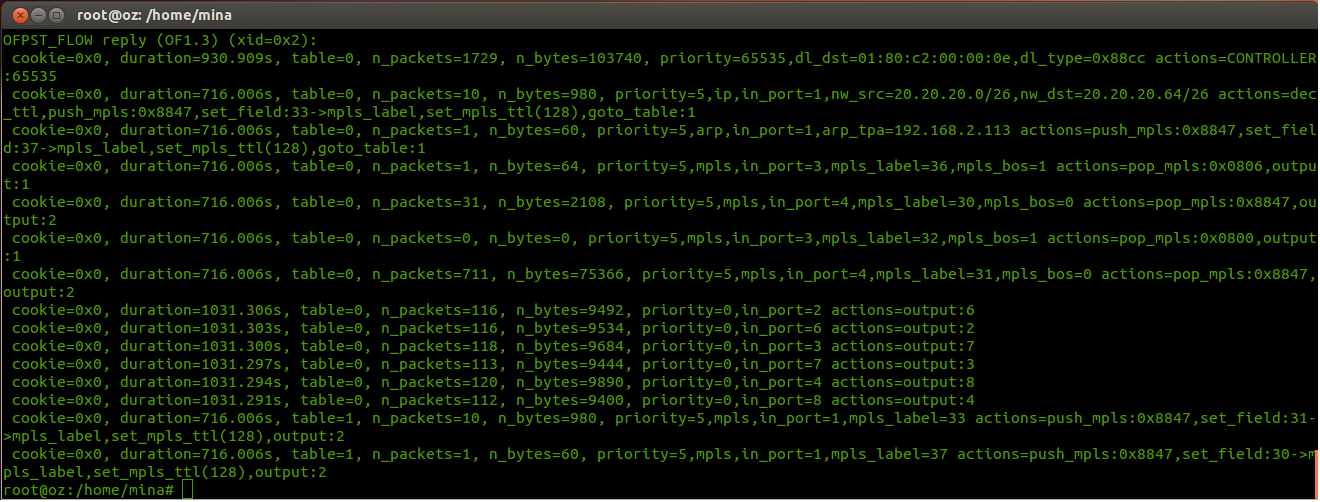
\includegraphics[width=1.0\textwidth]{E2P1Oz}
\caption[Tabla de flujos ovs - Oz]{Tabla de flujos ovs - Oz}
\label{fig:CU1P1DumpFlows2}
\end{figure}

\begin{figure}[h!] 
\centering    
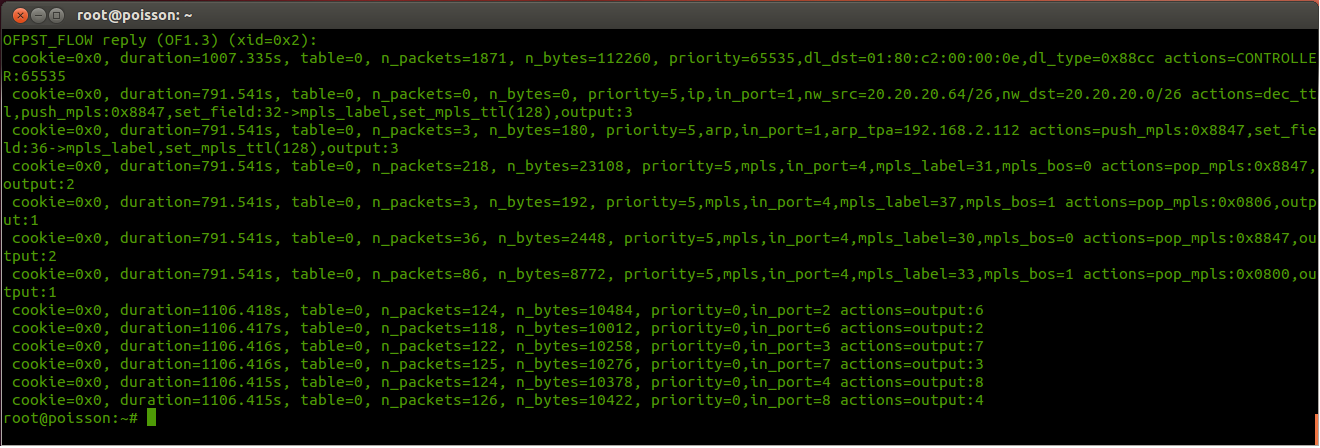
\includegraphics[width=1.0\textwidth]{E2P1Poi}
\caption[Tabla de flujos ovs - Poisson]{Tabla de flujos ovs - Poisson}
\label{fig:CU1P1DumpFlows3}
\end{figure}

\begin{figure}[h!] 
\centering    
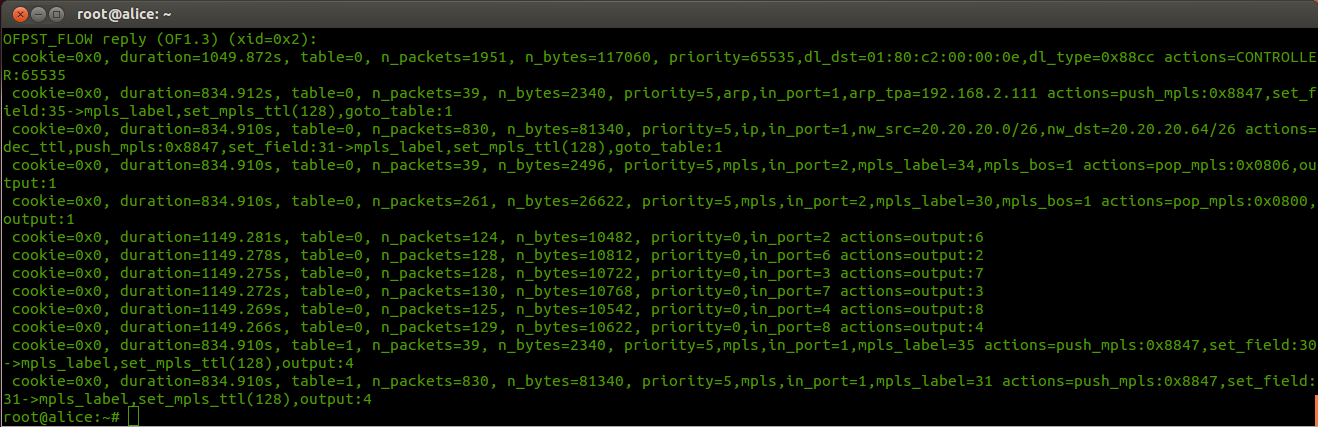
\includegraphics[width=1.0\textwidth]{E2P1Al}
\caption[Tabla de flujos ovs - Alice]{Tabla de flujos ovs - Alice}
\label{fig:CU1P1DumpFlows4}
\end{figure}

llalala

\newpage
\section{VPN de capa 2}

%\chapter{Gestión del proyecto}

% **************************** Define Graphics Path **************************
\ifpdf
    \graphicspath{{Chapter7/Figs/Raster/}{Chapter7/Figs/PDF/}{Chapter7/Figs/}}
\else
    \graphicspath{{Chapter7/Figs/Vector/}{Chapter7/Figs/}}
\fi

En el presente cap\'itulo se realiza un breve análisis acerca de la ejecuci\'on del proyecto, mostrando de las principales actividades y l\'ineas de trabajo seguidas, las respectivas fechas de inicio y fin de las actividades, destacando en los casos en que corresponde las posibles dependencias y atrasos.

\section{Ejecuci\'on del proyecto}

En la figura \ref{fig:gantt} se muestra un diagrama de Gantt con las actividades m\'as importantes durante la ejecuci\'on de este proyecto, con sus respectivas fechas de inicio y fin.

\begin{figure}[h!] 
\centering    
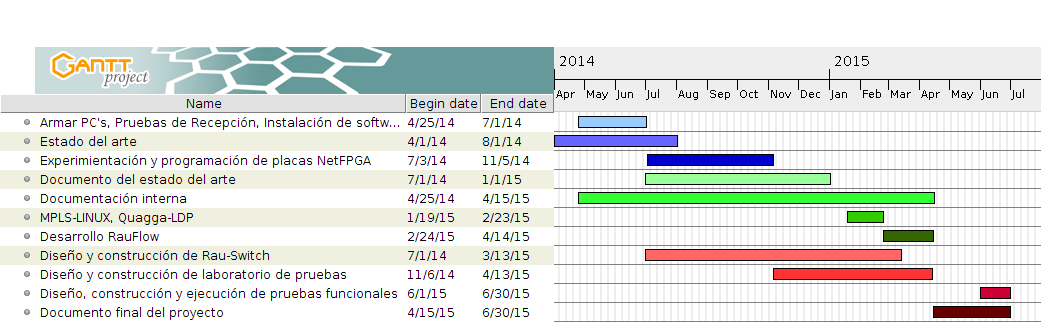
\includegraphics[width=1.00\textwidth]{ganttDP}
\caption[Diagrama de Gantt, Actividades del Proyecto]{Diagrama de Gantt, Actividades del Proyecto}
\label{fig:gantt}
\end{figure}

A continuaci\'on se describen los principales contratiempos experimentados en la ejecuci\'on de cada una de estas actividades.\\

\textbf{Armar PC's, Pruebas de Recepción, Instalación de software b\'asico:} Esta l\'inea de trabajo engloba las actividades realizadas al inicio del proyecto en las que se monta la plataforma base de cuatro dispositivos RAU-Switch utilizados adem\'as como estaci\'on de trabajo durante toda la ejecuci\'on del proyecto. En esta etapa se recibe el hardware utilizado (PC's, tarjetas NetFPGA, transceiver SFP y patch cords de fibra entre otros), se realiza un inventario, pruebas de aceptaci\'on y se procede con la instalaci\'on del hardware y software b\'asico (Sistema Operativo, suite de desarrollo de Xilinx entre otros).

Dentro de esta etapa son cr\'iticas la recepci\'on de todos los dispositivos de hardware y las pruebas de recepci\'on. Cabe destacar sobre esto, el 14/04/2014 se reciben las primeras dos PC's con las cuales empezar a trabajar, mientras que en la primera semana del mes de Junio llegan cinco placas NetFPGA.\\

\textbf{Estado del Arte:} Esta l\'inea de trabajo se desarrolla sin contratiempos aunque se extiende un mes m\'as de lo previsto cuando comienza la etapa de experimentaci\'on con el hardware.\\
  
\textbf{Experimentaci\'on y programaci\'on de las placas NetFPGA:} Esta linea de trabajo engloba actividades como la programaci\'on del hardware con los diferentes proyectos disponibles (de referencia y comunitarios), aprendizaje del entorno de desarrollo, evaluar la posibilidad de programar directamente el hardware con desarrollos propios, diseñar una estrategia de implementaci\'on para RAU-Switch.

Dentro de esta etapa es cr\'itica la obtenci\'on de un paquete de licencias pagas especiales para la suite de Xilinx ISE SDK. Oficialmente se obtiene este paquete el 29/10/2014 aunque el 16/10/2014 se obtiene una soluci\'on provisoria a este problema. A su vez es cr\'itico de esta etapa completar la programaci\'on persistente del hardware sin errores en el funcionamiento, hecho que sucede el día 05/11/2014.\\

\textbf{Documento del estado del Arte:} Esta actividad se realiza en paralelo con el resto de las actividades del proyecto, teniendo dos iteraciones para la generación de un documento del estado del arte previo al expuesto en el informe final del proyecto. Estas son el 15/09/2014 y el 01/12/2015.\\

\textbf{Documentación interna:} Esta actividad se desarrolla en el transcurso de todo el proyecto orientada a la redacci\'on del documento final del proyecto.\\

\textbf{MPLS-Linux, Quagga-LDP:} Esta l\'inea de trabajo engloba las actividades de experimentaci\'on realizada con ambas herramientas durante la fase de construcci\'on de RAU-Switch. A pesar del tiempo invertido en esta actividad no se obtienen los resultados esperados y se decide abandonar esta l\'inea de trabajo sopesando el tiempo invertido.

Esta actividad es cr\'itica en el desarrollo de RAUFlow no permitiendo comenzar con esta \'ultima hasta que se finalizara.\\

\textbf{Desarrollo de RAUFlow:} Esta l\'inea de trabajo engloba las actividades de diseño e implementaci\'on de RAUFlow. Se invierte poco m\'as de un mes en esta actividad debido al atraso general en el cronograma del proyecto, sacrificando un conjunto bastante interesante de funcionalidades de la aplicaci\'on.\\

\textbf{Diseño y construcci\'on de RAU-Switch:} Esta l\'inea de trabajo engloba actividades de programaci\'on, experimentaci\'on e investigaci\'on con diferentes herramientas de software y el hardware utilizado, hasta alcanzar la construcci\'on del dispositivo en cuesti\'on. Como etapa en el proyecto comienza una vez que se finalizan las pruebas de recepci\'on de hardware y finaliza una vez que se alcanza un producto estable funcionalmente.

Como etapa de proyecto son cr\'iticas las pruebas de recepci\'on de hardware, las cuales habilitan una vez concluidas a comenzar a trabajar en la misma.\\

\textbf{Diseño y construcci\'on del laboratorio de pruebas:} Comienza como etapa cuando culmina la etapa de experimentaci\'on con el hardware y comienza a pensarse en el diseño de RAU-Switch y de un laboratorio de pruebas utilizando los cuatro nodos disponibles y culmina el 13/04/2015 cuando se reciben las \'ultimas componentes de hardware necesarias para la construcci\'on del mismo.\\

\textbf{Diseño, implementaci\'on y ejecuci\'on de pruebas funcionales:} Engloba todas las actividades de verificaci\'on del prototipo construido utilizando el laboratorio de pruebas.

Son cr\'iticas para realizar las actividades de ejecuci\'on de pruebas el contar con el laboratorio de pruebas construido y una versi\'on estable de RAUFlow.\\

\textbf{Documentaci\'on del proyecto:} Si bien a lo largo de todo el proyecto se genera documentaci\'on, es de carácter interno. La elaboraci\'on del documento final de proyecto se posterga hasta el momento de contar con una versi\'on estable de RAUFlow, lo cual sucede el 15/04/15.\\
%\chapter{Conclusiones}

% **************************** Define Graphics Path **************************
\ifpdf
    \graphicspath{{Chapter8/Figs/Raster/}{Chapter8/Figs/PDF/}{Chapter8/Figs/}}
\else
    \graphicspath{{Chapter8/Figs/Vector/}{Chapter8/Figs/}}
\fi

En este cap\'itulo se resumen los principales resultados, logros y conclusiones de este trabajo. Luego se enumeran las principales l\'ineas de trabajo a futuro identificadas, entre las cuales se incluyen mejoras y extensiones al prototipo, como posibles l\'ineas de investigaci\'on.

\section{Conclusiones}
Se realiz\'o una investigaci\'on en profundidad del estado del arte de las redes definidas por software  
 (SDN) y la plataforma de hardware NetPGA, presentando un res\'umen de los resultados obtenidos en el cap\'itulo 2 de este trabajo.

Por otro lado se logr\'o desarrollar un prototipo funcional utilizando el hardware NetFPGA y el enfoque de SDN, dotado de funcionalidades para la creaci\'on y gesti\'on de servicios de redes privadas virtuales. Este prototipo es la prueba de que es posible implementar una red IP/MPLS en la que la inteligencia de los dispositivos de red convencionales es extra\'ida y colocada en una entidad centralizada.

El prototipo alcanzado se compone de un dispositivo de red denominado RAU-Switch y una aplicaci\'on de gesti\'on denominada RAUFlow. Orientado a una futura reproducci\'on de este trabajo, se gener\'o un manual de construcci\'on de RAU-Switch donde se detallan todas las componentes de hardware y software utilizadas, junto con el procedimiento de instalaci\'on y configuraci\'on de las mismas, para obtener un dispositivo id\'entico al desarrollado en este trabajo. Adem\'as se cre\'o un sitio del proyecto en la plataforma Github (Proyecto RRAP\cite{GitRRAP}) en donde se comparti\'o con la comunidad el c\'odigo fuente de todas las componentes de software desarrolladas en el marco de este proyecto, el conocimiento y experiencia generados en relaci\'on a las herramientas utilizadas. 

Por otro lado se diseñ\'o e implement\'o un laboratorio de experimentaci\'on sobre el cual se ejecutaron una serie de pruebas orientadas a la validaci\'on funcional del prototipo referidas a dos casos de uso representativos, ellos fueron la configuración de una VPN de capa 3 multipunto y una VPN de capa 2 punto a punto, sobre los cuales a su vez se ejecutaron una serie de pruebas para verificar la correcta implementaci\'on. De esta forma se logr\'o validar en lo que concierne a los requerimientos planteados, la aplicabilidad del enfoque SDN en la construcci\'on de la RAU2.

Adem\'as se gener\'o una publicaci\'on cient\'ifica en la cual se presentan los resultados obtenidos por este trabajo en el contexto de la construcci\'on de un prototipo para la RAU2 bajo el nombre "RAU2 testbed: a network prototype for evolved service experimentation" \cite{RauflowArticle}. Este art\'iculo fue presentado en la conferencia Latin American Network Operations and Management Symposium (LANOMS) y aceptado en formato de poster.

No menos importante, se logr\'o integrar el equipo de desarrollo con la comunidad de NetFPGA a trav\'es de la participaci\'on en la lista oficial de correos; contribuyendo desde la experiencia obtenida en la contestaci\'on de dudas y reportando dos errores importantes en el proyecto ReferenceNIC. A su vez se gener\'o un grupo de trabajo local integrando profesionales del SeCIU, Centro de Capacitaci\'on y Desarrollo de ANTEL y del Centro Universitario de la Regi\'on Este (CURE), en el cual se organizaron reuniones quincenales durante un per\'iodo de casi ocho meses para la puesta en com\'un y generaci\'on de experiencia y conocimiento en el \'area de SDN.

Finalmente, pese q que el dispositivo RAU-Switch diseñado est\'a fuertemente limitado en su rendimiento y performance por su implementaci\'on mayoritariamente en software y a pesar de que no se pudieron realizar pruebas comparativas con productos comerciales similares en funcionalidades, se logr\'o validar la utilizaci\'on de esta plataforma en la construcci\'on de un dispositivo compatible con OpenFlow. Adem\'as se identific\'o el camino a seguir para la construcci\'on de un prototipo con mejores prestaciones explotando al m\'aximo las capacidades del hardware disponible.  

\section{Trabajo a futuro}
En este trabajo no se compara el rendimiento del prototipo con productos comerciales similares en funcionalidades dado que estos implementan el plano de datos de OpenFlow en hardware, mientras que el prototipo lo implementa en software (Open vSwitch). De esta forma los tiempos de rendimiento ser\'ian incomparables.

Por ello interesa fuertemente extender el proyecto OpenFlow de la plataforma NetFPGA para que implemente el protocolo como mínimo en la versi\'on 1.3.1 y as\'i poder realizar una evaluaci\'on experimental que permita validar desde el punto de vista del rendimiento la aplicaci\'on de las tecnolog\'ias utilizadas en la construcci\'on de la RAU2.

El algoritmo de ruteo implementado basa su m\'etrica solamente en el costo asociado a un enlace de red. Extender la definici\'on de esta m\'etrica, contemplando otros atributos de un enlace como el ancho de banda disponible o tecnolog\'ia (fibra \'optica, enlace de cobre, etc) y a la vez contemplar restricciones como garantizar un ancho de banda m\'inimo, cantidad de enlaces atravesados, incluir \'o excluir nodos por los que pasar\'a el tr\'afico y demoras de extremo a extremo (en otras palabras implementar un CSPF) redituaría en la capacidad para incorporar funcionalidades de calidad de servicio.

De la mano de la extensi\'on del algoritmo de ruteo a un algoritmo CSPF, se puede trabajar en el desarrollo de funcionalidades avanzadas que permitan implementar t\'ecnicas de Ingenier\'ia de Tr\'afico, desarrollando as\'i un prototipo m\'as flexible en la asignaci\'on de los recursos disponibles y con mejor calidad en los servicios brindados.

Un servicio queda definido en el sistema por los nodos e interfaces de entrada y salida a la red y las caracter\'isticas del tr\'afico asociado. La incorporaci\'on de nuevas dimensiones a la definici\'on de un servicio, como dimensiones de calidad de servicios (QoS) o simplemente la dimensi\'on tiempo representar\'ia una gran mejora funcional y un salto de calidad en el aprovechamiento de las capacidades de la infraestructura del prototipo. Por ejemplo incorporando la dimensi\'on tiempo se podr\'ian definir servicios para rangos horarios, mejorando la precisi\'on con la que se distribuye el ancho de banda disponible.

En el prototipo se almacena en memoria informaci\'on que es ingresada por un usuario de la aplicaci\'on RAUFlow. En particular se almacenan datos extra de cada nodo e interfaz y se almacena la definici\'on de los servicios. Esta informaci\'on se pierde en caso de que la aplicaci\'on sea interrumpida puesto que no se persiste de forma no volátil. Resulta interesante entonces incorporar a la arquitectura de RAUFlow una capa de persistencia que permita guardar de forma no vol\'atil esta informaci\'on, adem\'as de la definici\'on de estrategias para la reconstrucci\'on de servicios cuando se carga esta informaci\'on eventualmente en una topolog\'ia de red diferente a la inicial.

Almacenar en memoria y de forma centralizada la informaci\'on topol\'ogica de red, informaci\'on asociada a servicios y eventualmente funcionalidades de QoS e Ingenier\'ia de tr\'afico, as\'i como ejecutar algoritmos que utilicen intensivamente estos datos como un CSPF centralizado puede acarrear serias barreras de escalabilidad en el prototipo. Una l\'inea de investigaci\'on interesante ser\'ia el desarrollo de una jerarqu\'ia de Controladores, cada uno responsable del plano de control de una porci\'on de la topolog\'ia global. De esta forma se generar\'ian islas SDN en donde el tr\'afico interno es resuelto por el controlador local y se consulta al Controlador global para resolver la forma en que se enruta tr\'afico entre diferentes islas. A su vez se puede crecer en la cantidad de niveles dentro de la jerarqu\'ia tanto como se quiera.

Finalmente y no menos importante se puede trabajar en el desarrollo de nuevas funcionalidades en RAUFlow, así como en la mejora de las ya existentes. Algunas de las funcionalidades que se pueden incorporar son la capacidad para definir manualmente caminos, indicando los nodos por los que se quiere  
pasar, soportar m\'ultiples caminos para un mismo par de nodos origen y destino y as\'i poder implementar balanceo de carga, creaci\'on de una VPN multipunto autom\'aticamente a partir de una lista de nodos e interfaces involucradas. 


%\chapter{Conclusiones}

% **************************** Define Graphics Path **************************
\ifpdf
    \graphicspath{{Chapter9/Figs/Raster/}{Chapter9/Figs/PDF/}{Chapter9/Figs/}}
\else
    \graphicspath{{Chapter9/Figs/Vector/}{Chapter9/Figs/}}
\fi


asdsadasdsa
asasdsaadsasdsad



% ********************************** Back Matter *******************************
% Backmatter should be commented out, if you are using appendices after References
%\backmatter

% ********************************** Bibliography ******************************
\begin{spacing}{0.9}

% To use the conventional natbib style referencing
% Bibliography style previews: http://nodonn.tipido.net/bibstyle.php
% Reference styles: http://sites.stat.psu.edu/~surajit/present/bib.htm

\bibliographystyle{apalike}
%\bibliographystyle{plainnat} % use this to have URLs listed in References
\cleardoublepage
\bibliography{References/references} % Path to your References.bib file


% If you would like to use BibLaTeX for your references, pass `custombib' as
% an option in the document class. The location of 'reference.bib' should be
% specified in the preamble.tex file in the custombib section.
% Comment out the lines related to natbib above and uncomment the following line.

%\printbibliography[heading=bibintoc, title={References}]


\end{spacing}

% ********************************** Appendices ********************************

\begin{appendices} % Using appendices environment for more functunality

%% ******************************* Thesis Appendix A ****************************
\chapter{Soluci\'on a errores encontrados en la plataforma NetFPGA} 

Durante el tiempo que se trabajo con el hardware NetFPGA, se detectaron errores y comportamientos inesperados en el mismo. En particular se encontraron errores de severidad alta en relaci'on al  impacto sobre el prototipo; durante el proceso de programaci\'on persistente del hardware con el proyecto ReferenceNIC.\\

En total se detectaron dos bugs, los cuales fueron reportados a la comunidad de NetFPGA y al equipo de soporte atraves de la lista de correos. El equipo de NetFPGA r\'apidamente confirmo los mismos,
ofreciendonos soluciones a ambos errores. Luego se constato que estos errores fueron solucionados en la siguiente versi\'on del c\'odigo fuente de la plataforma.\\ 

Cabe destacar que estos errores fueron detectados trabajanfo con la versi\'on 5.0.5 del c\'odigo fuente.
 
\section*{Problema con la herramienta pcieprog y ReferenceNIC}
El primer error detectado se encuentra en la herramienta \textbf{pcieprog} dentro de la plataforma de NetFPGA. La misma se utiliza para transferir el archivo binario generado a partir del bitfile del proyecto (en este caso ReferenceNIC) a una de las memorias Flash del hardware.

Al ejecutarse esta herramienta con el binario generado para el proyecto ReferenceNIC, la misma se estancaba durante horas con un 100\% de utilizaci\'on de la CPU. Tras probar con varias ejecuciones de la misma herramienta, se realizo la misma prueba con dos proyectos m\'as (reference\_ switch y reference\_ router), compatibles con la programaci\'on persistente. 

Para estos proyectos no se detecto el mismo comportamiento an\'omalo, por lo que se presumi\'o la presencia de un bug en el c\'odigo del proyecto ReferenceNIC. A su vez se procedio con la inspecci\'on del c\'odigo de la herramienta \textbf{pcieprog}, hasta que finalmente se logro aislar la porci\'on del mismo donde el programa se estancaba. En particular el programa quedaba estancado en un loop infinito porque no se cumplia la condici\'on de salida nunca.\\ 

Este comportamiento fue reportado al grupo de soporte a traves de una lista de correos(ver correos en anexo [link al anexo]), obteniendose el siguiente parche para solucionar el problema:

\begin{enumerate}
\item Dentro del directorio donde se encuentra el c\'odigo fuente de la plataforma, posicionarse en 
	  projects/reference\_nic/hw/. Abrir el archivo system.mhs.\\
	  Cambiar:
\begin{center}
	"PORT axi\_ emc\_ 0\_ Mem\_ DQ\_ pin = axi\_ emc\_ 0\_ Mem\_ DQ, DIR = IO, VEC = [*7*:0]"
\end{center}
por
\begin{center}
"PORT axi\_ emc\_0 \_Mem\_ DQ\_ pin = axi\_ emc\_ 0\_ Mem\_ DQ, DIR = IO, VEC = [*31*:0]"
\end{center}

\item Posicionarse ahora en projects/reference\_nic/hw/. Abrir el archivo xflow.opt.\\
	  Cambiar:
\begin{center}
"-t *1*"
\end{center}
por
\begin{center}
"-t *5*"
\end{center}

\item Recompilar el proyecto ReferenceNIC ejecutando el comando make en el directorio projects/reference\_ nic/

\item Utilizar el nuevo bitfile generado para programar el hardware, generar un nuevo archivo binario y transerir a la memoria Flash.
\end{enumerate}

\section*{Error en driver para ReferenceNIC}
El segundo error detectado con este proyecto, tambi\'en en la modalidad de programaci\'on persistente  se encuentra relacionado al driver utilizado para la interacci\'on entre el hardware y el sistema operativo anfitrion.\\

Este error fue detectado experimentalmente al realizar pruebas de funcionamiento entre varios nodos utilizando el hardware programado con el proyecto ReferenceNIC, y se detalla a continuaci\'on:

\begin{itemize}
\item \textbf{Descripci\'on:}\\
Al programarse el hardware con el proyecto ReferenceNIC desde la memoria Flash utilizando la programaci\'on pcie, no funciona correctamente cuando la placa NetFPGA tiene conectados enlaces en sus puertos. En particular para que el hardware funcione correctamente debe ser encendido sin cables conectados en los puertos, y luego conectar manualmente cada uno de ellos una ves que el equipo completo el encendido.

\item \textbf{Escenario:}
\begin{itemize}
\item Dos PCs cada una con una tarjeta NetFPGA instalada
\item Las tarjetas estan conectadas por cuatro enlaces de fibra \'optica (nf0-nf0, nf1-nf1, nf2-nf2 y nf3-nf3)
\item Ambas tarjetas estan programadas con el proyecto ReferenceNIC via programaci\'on pcie.
\item Se utiliza la versi\'on 5.0.5 de c\'odigo fuente, con el parche mencionado anteriormente.
\end{itemize}

\item \textbf{Efecto:}\\
Incapacidad parar ejecutar exitosamente el comando ping entre cualquier par de interfaces conectadas

\item \textbf{Reproducci\'on:}\\
Partiendo de ambas PCs apagadas
\begin{enumerate}
\item Encender una de las PC, teniendo conectados los enlaces \'opticos entre ambas PCs
\item Cargar el driver nf10 y configurar manualmente direcciones IP para cada interaz (nf0 \dots nf3)
\item Luego realizar el mismo procedimiento para la otra PC
\item Leds asociados a cada puerto en una de las tarjetas NetFPGA son encendidos por completo, mientras que en la otra tarjeta solamente la mitad de los Leds se encuentran encendidos.
\item Si se apaga y enciendo la PC con la tarjeta NetFPGA cuyos leds se encuentran todos prendidos, luego la otra tarjeta enciende todos sus leds, mientras que la primera enciende solo la mitad de sus leds. 
\item El \'ultimo paso puede repetirse, y el comportamiento observado se mantiene. En particular la tarjeta que es iniciada al final funciona correctamente mientras que la otra no.
\end{enumerate} 

\item \textbf{Soluci\'on:}
\begin{enumerate}
\item Apagar ambas PCs
\item Desconectar todos los enlaces \'opticos
\item Encender ambas PCs(cargar el driver nf10 y configurar cada interfaz con una direcci\'on IP apropiada)
\item Luego de que cada PC esta encendida y configurada conectar los enlaces \'opticos uno a uno.
\end{enumerate}

\end{itemize}

Este reporte tambi\'en fue enviado a la comunidad de NetFPGA (ver anexo con emails [link al email]), en donde se constato nuevamente la presencia de un error, esta vez en la configuraci\'on de los chips PHY de la tarjeta. 

La soluci\'on planteada por el equipo de NetFPGA fue la siguiente:

\begin{enumerate}
\item Dentro del directorio donde se encuentra el c\'odigo fuente de la plataforma, posicionarse en 
	  projects/reference\_ nic/sw/host/driver/. Abrir el archivo nf10\_ phy\_ conf.c .
\item Comentar las lineas 217,219 y 240.
\item Recompilar el driver nf10
\item Reiniciar la PC y cargar el nuevo driver
\end{enumerate}

Tras esta correcci\'on el proyecto ReferenceNIC funciona correctamente, comportandose el hardware como una tarjeta de red convencional. A su vez cada vez que la PC es encendida el hardware se reprograma desde la memoria flash apropiadamente.

%Cabe destacar que este procedimiento no funciona correctamente. El proyecto PCIPrograming presenta alg\'un tipo de BUG(al momento de grabar una memoria se queda en loop), y tras reportar este comportamiento en la comunidad de NetFPGA se nos suguiere utilizar el proyecto ReferenceNIC que presenta el diseno de la arquitectura similar al PCIPrograming. Siguiendo esta sugerencia se logra programar correctamente el hardware de forma persistente, constatandose que al realizar un ciclo de corriente completo el hardware no se desprograma. Por esta raz\'on la estrategia de programaci\'on utilizada en el hardware es la programaci\'on persistente aqu\'i detallada.\\

%Vale la pena destacar tambi\'en, que al programarse el hardware desde cualquiera de las unidades de memoria Flash, en particular con el proyecto Reference NIC el hardware no se comportaba de la forma esperada. Tras constatarse que esto no sucedia con versiones anteriores del c\'odigo fuente del proyecto, nuevamente se le reporta lo sucedido al soporte de NetFPGA obteniendo como respuesta una sugereencia para emparchar el c\'odigo, y la promesa de que ser\'ia solucionado en la siguiente versi\'on (lo cual pudimos constatar).

%Tras estas modificaciones se logra obtener el hardware programado de forma persistente. De todos modos luego de ejecutarse una serie de pruebas se constatan comportamientos an\'omalos en capa f\'isica de las interfaces de la placa (podemos meter la descripcion). Nuevamente se reporta el comportamiento a la comunidad de NetFPGA desde donde se nos suguiere un parche para el driver, aparentemente causante del error. Se realizan los cambios y todo anda yuju!  
%% ******************************* Thesis Appendix B ********************************

\chapter{Desaf\'ios t\'ecnicos encontrados}

% **************************** Define Graphics Path **************************
\ifpdf
    \graphicspath{{Appendix2/Figs/Raster/}{Appendix2/Figs/PDF/}{Appendix2/Figs/}}
\else
    \graphicspath{{Appendix2/Figs/Vector/}{Appendix2/Figs/}}
\fi

Durante la ejecuci\'on del proyecto, nos enfrentamos a desaf\'ios y en particular de carácter t\'ecnico. Dentro de estos desaf\'ios podemos encontrar algunos que se destacan por su complejidad y dificultad para resolverlos y otros que se destacan por su severidad como riesgo tecnol\'ogico dentro del proyecto. Por ello consideramos apropiado incluir un ap\'endice en donde se hace menci\'on a los mismos y a sus respectivas soluciones.

\section{Problemas con SFPs y Patchcoords}

Los transceivers SFP+ son una componente de hardware utilizada en cada puerto f\'isico de la tarjeta NetFPGA en la construcci\'on del dispositivo RAU-Switch. Básicamente se encargan de implementar el mecanismo de acceso a la capa f\'isica, en este caso fibra \'optica.

Pueden encontrarse transceivers compatibles con patch cords de fibra \'optica monomodo, multimodo y compatibles con ambos tipos.

En el desarrollo de este proyecto se trabaj\'o con transceivers SFP+ compatibles con ambos tipos de patch cords, aunque para la construcci\'on de la red prototipo por razones econ\'omicas se utilizaron transceivers SFP+ compatibles solamente con patch cords de fibra multimodo.

\section{Desprogramaci\'on del hardware NetFPGA}
\label{apendiceB2}

En el desarrollo de este proyecto se utilizan dos estrategias diferentes para programar el hardware NetFPGA. La primera estrategia, detallada en la guía de ejecución del Test de Producción\citep{ProdTestManual}, permite de forma sencilla programar el hardware utilizando la herramienta Impact de la suite Xilinx ISE SDK. Sin embargo este procedimiento no persiste la programaci\'on del hardware, por lo que al producirse un corte de corriente en el circuito (apagado de la PC por ejemplo) el mismo pierde la programaci\'on. Este efecto puede comprobarse fácilmente utilizando la herramienta Impact para leer el valor de diferentes registros del hardware, los cuales indican el estado del mismo.

La segunda estrategia es la programación PCIe denominada en este trabajo como programación persistente, la cual utiliza la herramienta \textbf{pcieprog} de la plataforma NetFPGA para almacenar la programaci\'on del hardware en una de las unidades de memoria Flash del equipo. Concretamente este procedimiento implica programar el hardware con un proyecto compatible con la programaci\'on PCIe (es necesario que el proyecto implemente un m\'odulo para la configuraci\'on del chip FPGA desde una de las memorias Flash) utilizando la herramienta Impact. Luego se almacena en una de las unidades de memoria Flash un archivo binario con la implementaci\'on del proyecto con el cual se quiere programar el hardware. Luego al momento del encendido del equipo, el chip FPGA es programado desde el contenido almacenado en una de las memorias Flash.

De esta forma la programaci\'on del equipo se almacena de forma persistente, perdurando incluso cuando el equipo es apagado.

\section{Falta de licencias para suite de Xilinx ISE SDK}
\label{apendiceB3}
La suite de desarrollo Xilinx ISE SDK se compone por un conjunto extenso de herramientas para la progrmaci\'on y desarrollo de software utilizando los productos de este fabricante; entre los cuales se encuentra el chip Virtex 5 utilizado en el hardware NetFPGA. Estas herramientas de software son licenciadas lo que significa que para su uso es necesario contar con una licencia de software apropiada.

Cada herramienta particular de la suite Xilinx tiene una licencia particular y se agrupan en diferentes paquetes de licencias. De esta forma dependiendo del uso que se vaya a hacer de esta plataforma, el o los paquetes de licencias que se deben adquirir. Adem\'as cada licencia se corresponde con una herramienta para una familia de chips en particular. Por ejemplo para trabajar con las tarjetas NetFPGA-10G se necesitan licencias para el chip Virtex5 TX240T.

Xilinx ofrece un paquete de licencias gratuitas para trabajar con un conjunto reducido de herramientas (entre ellas se incluye el programa Impact) y un paquete de licencias completo de prueba por un tiempo de 30 d\'ias compatible con los \'ultimos modelos de chips (Virtex6 y Virtex7). Como dentro de estos paquetes no se incluyen las licencias necesarias para la programaci\'on PCIe (programaci\'on persistente) una alternativa es adquirir un paquete de licencias con un valor aproximado de USD500 por PC (costo en dolares americanos al mes de Setiembre del año 2014).

En este proyecto, por razones econ\'omicas primero se solicit\'o mediante el programa de soporte a Universidades de Xilinx el paquete de licencias necesario, a la vez que se inici\'o un contacto con el Instituto de Ingeniería Eléctrica de la Facultad de Ingeniería (IIE) solicitando orientación en relación a este problema. Finalmente se recibi\'o a través de dicho programa de apoyo a universidades una interesante donación de licencias, posibilitando una real explotación del hardware y la plataforma en su conjunto, aunque esta espera represent\'o un contratiempo en el cronograma inicial del proyecto. 

\section{Falta de driver para cable JTAG Xilinx}
Para la programación del hardware NetFPGA se utiliza un cable programador especial con una interfaz de conexi\'on JTAG.  Este cable presenta el inconveniente de que sus fabricantes no desarrollaron drivers para la distribución de Linux con la que se trabaja en este proyecto, existiendo drivers oficiales para entornos Windows y una versi\'on no oficial para la distribución Fedora.

Si bien inicialmente esto oblig\'o a programar el hardware en un ambiente Windows para realizar las pruebas de verificaci\'on del mismo (Producction Test y RLDRAM Test) finalmente se consigue un driver no oficial\cite{JtagD} tambi\'en compatible con Ubuntu 12.04, habilitando de esta forma a programar el hardware en la misma PC.

\section{Problemas t\'ecnicos con Open vSwitch}
\label{apendiceB5}

Open vSwitch es uno de los pilares fundamentales de RAU-Switch puesto que es el encargado de implementar el plano de datos de OpenFlow. Durante el desarrollo de este proyecto, en el tiempo empleado a la experimentaci\'on con esta herramienta, se genera conocimiento en relaci\'on a aspectos importantes sobre la herramienta; los cuales no son triviales y vale la pena mencionar en este apartado. A continuaci\'on se enumeran los siguientes:

\begin{enumerate}
\item Parte de las funcionalidades de Open vSwitch, est\'an implementadas en modo kernel y otra parte en modo usuario. Estas \'ultimas presentan un nivel de performance muy pobre en comparaci\'on a las primeras; y en particular las funcionalidades de MPLS se encuentran solamente disponibles en modo usuario.

\item De acuerdo a la p\'agina de preguntas frecuentes, la \'ultima versi\'on de Open vSwitch al momento de realizarse este proyecto, garantiza soporte a las operaciones de MATCH, PUSH y POP de hasta tres etiquetas MPLS apiladas, as\'i como su posterior procesamiento acorde al pipe de OpenFlow. Todas estas funcionalidades adem\'as se implementan en modo usuario.

Por otro lado, de acuerdo  a las notas de liberaci\'on de la versi\'on 2.3.1, solamente se garantiza el soporte a las funciones de MATCH, PUSH y POP de MPLS para un \'unico nivel de etiquetas; esto es una sola etiqueta MPLS. Luego se garantiza adem\'as el posterior procesamiento acorde al pipe OpenFlow. Esta informaci\'on no s\'olo es contradictoria, sino que adem\'as no se condice con la realidad. Experimentalmente se prueba que si bien la versi\'on 2.3.1 implementa correctamente las operaciones de MATCH y PUSH de una \'unica etiqueta MPLS, la operaci\'on POP no se encuentra implementada para esta versi\'on, rompiendo adem\'as el pipe de procesamiento OpenFlow. 

Afortunadamente \'este comportamiento hab\'ia sido detectado y reportado por otros usuarios de Open vSwitch como un BUG, resolviéndose posteriormente en la versi\'on de desarrollo \citep{OVSSourceCode}.

\item Trabajando con la versi\'on de desarrollo en el repositorio de c\'odigo fuente de Open vSwitch~\citep{OVSSourceCode} (rama master en el repositorio Git), se comprueba experimentalmente el soporte para las operaciones de Match, Push y Pop de hasta 3 etiquetas, as\'i como el posterior procesamiento del paquete seg\'un el pipe de  OpenFlow.

\item Puertos OpenFlow con direcciones IP:
 
Para lograr que cada interfaz f\'isica de la tarjeta NetFPGA se comporte tanto como un puerto OpenFlow, como una interfaz IP, es necesario:

\begin{enumerate}
\item Crear un bridge con Open vSwitch y agregar cada interaz f\'isica como un puerto OpenFlow al mismo.
\item Asignar una dirección IP a la propia intefaz f\'isica (por ejemplo utilizando el comando ifconfig).
\end{enumerate}

El comportamiento deseado por una interfaz h\'ibrida IP/OpenFlow en el prototipo ser\'ia el que se muestra en la figura ~\ref{fig:OVSInterfaces} (mitad izquierda). El paquete ingresa al router atrav\'es de la interfaz f\'isica \textbf{nf0} y de ah\'i en m\'as el procesamiento del mismo es delegado al m\'odulo de Open vSwitch en el kernel de Linux. Aqu\'i el paquete es procesado y tratado en consecuencia a lo que indica la tabla de flujos en Open vSwitch. En el prototipo, para este paquete existen dos alternativas: (1) se procesa el contenido del mismo y se reenv\'ia por otra interfaz acorde a la regla correspondiente, (2) es contemplado por una regla con la acci\'on \textit{NORMAL} y por tanto es procesado como lo har\'ia un switch legado (en este caso como lo procesar\'ia el kernel de linux).

\begin{figure}[h!] 
\centering    
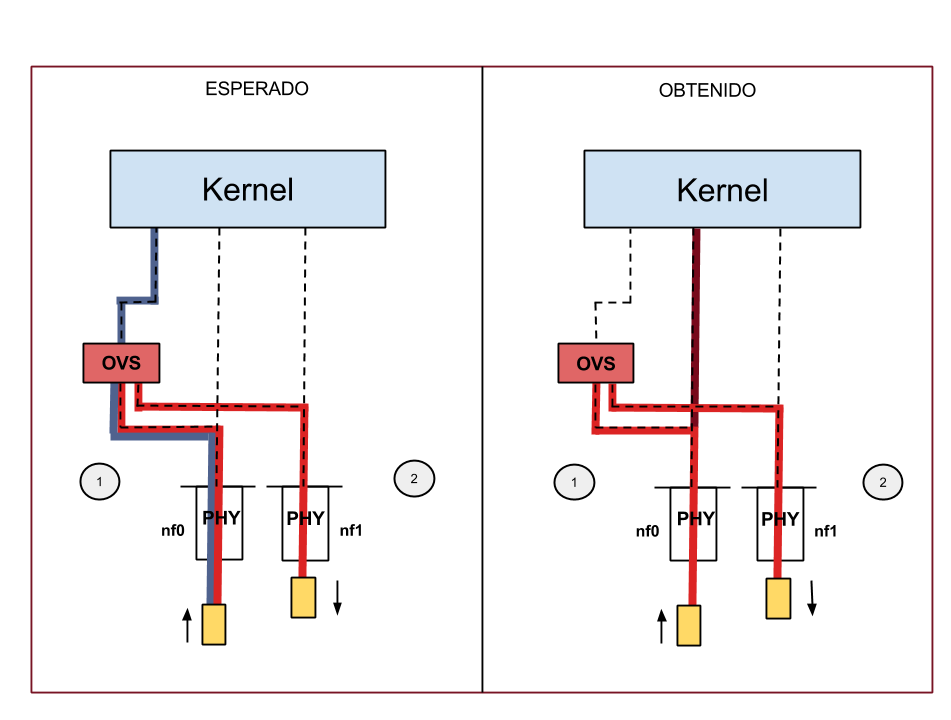
\includegraphics[width=0.60\textwidth]{ovs_figure3}
\caption[Funcionamiento de puertos Open vSwitch]{Funcionamiento de puertos Open vSwitch}
\label{fig:OVSInterfaces}
\end{figure}

No obstante, el procesamiento del paquete al ingresar por la interfaz f\'isica \textbf{nf0} difiere del comportamiento deseado (ver mitad derecha de la imagen). El paquete es procesado por Open vSwitch como se describi\'o anteriormente, pero tambi\'en es enviado para su procesamiento en el kernel de Linux.

Esto implica que el switch se comporte como una mezcla de un switch OpenFlow  con una PC Linux normal, ocasionando un tratamiento de paquetes en el prototipo diferente al especificado por las reglas OpenFlow calculadas.

Para solucionar este problema se utilizan interfaces virtuales de la siguiente forma:

\begin{enumerate}
\item Se crea una interfaz virtual por cada interfaz física y se conecta a través de dichas interfaces,  openvswitch con el kernel.

\item La dirección IP que antes se asignaba a cada interfaz física ahora se le asigna a su correspondiente interfaz virtual.

\item Se deja la interfaz física sin dirección IP y de esta forma se asegura que ningún paquete que arribe a dicha interfaz será procesado por el kernel, ya que nunca coincidirá la dirección IP que contenga un paquete con la dirección de la interfaz.

\item Se crean entradas de prioridad mínima en la tabla de flujos de openvswitch que indiquen que todo lo que entre por la interfaz física se envíe a través su correspondiente interfaz virtual y viceversa.

\item De esta forma si no hay un flujo de mayor prioridad para procesar los paquetes que entran por determinada interfaz física, estos serán enviados al kernel mediante la interfaz virtual, procesados por este para luego ser enviado por la interfaz virtual a la física y seguir su camino.

\item Estos pasos aseguran que todo el tráfico sea procesado por las tablas de Open vSwitch, y serán procesados por el kernel solo en caso de ser necesario.
\end{enumerate}

\begin{figure}[h!] 
\centering    
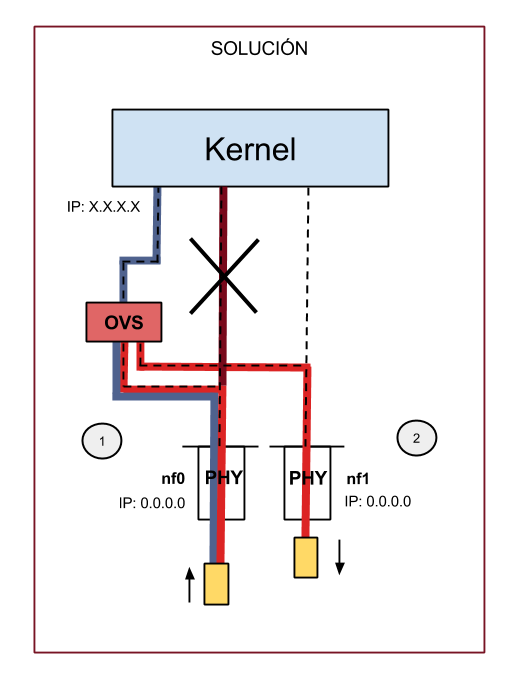
\includegraphics[width=0.33\textwidth]{ovs_figure4}
\caption[Puertos Open vSwitch - Soluci\'on propuesta]{Puertos Open vSwitch - Soluci\'on propuesta}
\label{fig:OVSInterfaces2}
\end{figure}

\end{enumerate}

\section{MPLS Linux y Quagga LDP}
\label{apendiceB6}

MPLS Linux es un proyecto orientado a dotar de funcionalidades de MPLS al Kernel de Linux, mediante un parche con el cual se extiende al mismo y el cual tras recompilarse queda pronto para brindar soporte nativo al protocolo MPLS.

Existen principalmente dos versiones: el proyecto original\cite{MplsLinux1} encabezado por James R. Leu el cual data de hace m\'as de 15 a\~nos y no cuenta con contribuciones importantes desde hace aproximadamente 9 y otro proyecto\cite{MplsLinux2} encabezado por Igor Maravick (quien trabaj\'o en el proyecto anterior) que data del a\~no 2010 y surge como una actualizaci\'on del proyecto original.

El primer proyecto fue pensado como un parche para el kernel de Linux versi\'on 2.6.3.16 (tener en cuenta que la versi\'on actual es la 4.1.1). Adicionalmente se desarroll\'o una extensión de la suite Quagga\cite{QuaggaLDP1} que implementa el algoritmo LDP para la construcci\'on de redes IP/MPLS.

Por otro lado, el proyecto de Igor Maravick es un kernel de Linux versi\'on 3.9.0-rc3 con las modificaciones necesarias para soportar el protocolo MPLS ya incorporadas. Adicionalmente existe una nueva extension de la suite Quagga que implementa el protocolo LDP \cite{QuaggaLDP2} y es compatible con esta versi\'on de MPLS-Linux.

En el contexto de este proyecto se trabaj\'o con ambas versiones de MPLS-Linux y las respectivas versiones de Quagga-LDP. Para la versi\'on original de MPLS-Linux se prob\'o compilar el parche con diferentes versiones de kernel, entre ellas las versiones 2.6.32.16 y 2.6.32.65 no pudiendo as\'i configurar correctamente el ambiente de trabajo. En particular estas versiones son tan antiguas que gran parte de las herramientas utilizadas para la construcci\'on de RAU-Switch no son compatibles. Adicionalmente se prueba compilar el parche para la versi\'on de kernel 3.11.0-15 generic (versi\'on que trae Ubuntu 12.01) pero tampoco se obtienen buenos resultados.

En relaci\'on a la versi\'on de Igor Maravik se logr\'o configurarla correctamente, as\'i como la extensi\'on Quagga-LDP. No obstante al momento de ejecutar dichas herramientas se detectaron problemas en la interacci\'on entre las mismas; mediante los logs de la herramienta Quagga se detectaron errores al momento de insertar entradas en las tablas MPLS del kernel.

Finalmente por la falta de información en relación a estas componentes, ya que sobre el proyecto original existe muy poca documentaci\'on mientras que para el proyecto de Igor Maravik no existe la misma, se decidi\'o descartar esta alternativa para implementar el algoritmo LDP. 
%% ******************************* Thesis Appendix C ********************************

\chapter{Clasificaci\'on de tr\'afico utilizando cabezales OpenFlow}
\label{appendix3}

En este ap\'endice se detallan de los atributos presentes en el cabezal OpenFlow versi\'on 1.3, cuales pueden ser utilizados para la definici\'on de reglas y cuales pueden ser utilizados en la definici\'on de acciones en un flujo. Esta informaci\'on es de carácter experimental y esta acotada a la compatibilidad de Open vSwitch; es decir, aquellos atributos que esta herramienta no soporta o simplemente no se consiguió documentaci\'on para entender su utilizaci\'on, no son considerados.

\section{Cabezal OpenFlow versi\'on 1.3} 

\begin{python}
of_v13_match_fields:
      
	in_port			# Switch input port.
	in_phy_port 	# Switch physical input port. 
	metadata 		# Metadata passed between tables. 
	eth_dst 		# Ethernet destination address.
	eth_src 		# Ethernet source address. 
	eth_type 		# Ethernet frame type. 
	vlan_vID 		# VLAN id. 
	vlan_PCP		# VLAN priority. 
	IP_dscp 		# IP DSCP (6 bits in ToS field). 
	IP_ecn  		# IP ECN (2 bits in ToS field). 
	IP_proto		# IP protocol. 
	IPv4_src 		# IPv4 source address. 
	IPv4_dst 		# IPv4 destination address. 
	TCP_src 		# TCP source port. 
	TCP_dst 		# TCP destination port. 
	UDP_src 		# UDP source port. 
	UDP_dst 		# UDP destination port. 
	SCTP_src 		# SCTP source port. 
	SCTP_dst 		# SCTP destination port. 
	ICMPv4_type 	# ICMP type. 
	ICMPv4_code 	# ICMP code. 
	ARP_op			# ARP opcode. 
	ARP_spa 		# ARP source IPv4 address. 
	ARP_tpa 		# ARP target IPv4 address. 
	ARP_sha 		# ARP source hardware address. 
	ARP_tha 		# ARP target hardware address. 
	IPv6_src 		# IPv6 source address. 
	IPv6_dst 		# IPv6 destination address. 
	IPv6_flabel 	# IPv6 Flow Label 
	ICMPv6_type 	# ICMPv6 type. 
	ICMPv6_code 	# ICMPv6 code. 
	IPv6_nd_target 	# Target address for ND. 
	IPv6_nd_ssl 	# Source link-layer for ND. 
	IPv6_nd_tll  	# Target link-layer for ND. 
	MPLS_label 		# MPLS label. 
	MPLS_tc 		# MPLS TC. 
	MPLS_bos		# MPLS BoS bit. 
	PBB_is_id 		# PBB I-SID. */
	tunnel_id 		# Logical Port Metadata. 
	IPv6_txhdr 		# IPv6 Extension Header pseudo-field 
		
\end{python}

Estos atributos fueron estudiados uno por uno y se llega a las dos listas presentadas en las siguientes secciones.\\

\section{Sintaxis de un flujo en Open vSwitch}
La sintaxis del comando ovs-ofctl, utilizado para agregar un flujo en la tabla de Open vSwitch es la siguiente:

\begin{center}
ovs-ofctl add-flow <bridge> <flow>
\end{center}

Los parámetros de este comando son el nombre del brdige (<bridge>) y el flujo definido. La sintaxis de un flujo es la siguiente:

\begin{center}
attr1\_name=<value>,attr2\_name=<value>,.. actions=<action1>,<action2>,...
\end{center}

Primero tiene una lista de pares atributo valor separados por una “,” las cuales definen la regla de un flujo; es decir, los campos del cabezal OpenFlow utilizados para aparear tr\'afico. Un ejemplo común es es utilizar el numero de puerto OpenFlow de entrada, in\_port=1 por ejemplo.

La segunda parte de un flujo es la lista de acciones, una lista de acciones precedida por la palabra \textbf{actions}. Un ejemplo común es reenviar paquetes por un puerto particular, por ejemplo out\_port:2. 
 
\section{OpenFlow v1.3 atributos soportados para definir reglas}

A continuaci\'on se detallan los atributos soportados para la definici\'on de reglas en un flujo lo cual en otras palabras permite la construcci\'on de una FEC y así clasificar tr\'afico.

\begin{itemize}

\item \textbf{in\_port}: Es utilizado para discriminar por el puerto de entrada en un switch

\item \textbf{metadata}: Es utilizado entre otras cosas para compartir informaci\'on entre varios flujos en diferentes tablas OpenFlow

\item \textbf{eth\_dst}: Permite a un flujo seleccionar tr\'afico distinguiendo por la direcci\'on destino de capa 2 (dirección MAC). EL valor utilizado se compone de 6 pares de hexadecimales.

\begin{center}
ovs-ofctl add-flow <bridge> dl\_dst=<mac>,actions=<action>
\end{center}

\item \textbf{eth\_src}: Permite a un flujo selecionar tr\'afico distinguiendo por direcci\'on origen de capa 2 (direcci\'on MAC). El valor utilizado se compone de 6 pares de hexadecimales.

\begin{center}
ovs-ofctl add-flow <bridge> dl\_dst=<mac>,actions=<action>
\end{center}

\item \textbf{dl\_type}: Permite a un flujo selecionar tr\'afico distinguiendo por el tipo de ethertype de un paquete. Se utiliza como valor el c\'odigo hexadecimal de cada protocolo.

\begin{center}
ovs-ofctl add-flow <bridge> dl\_type=<ethernet type>,actions=<action>
\end{center}

\item \textbf{vlan\_vID}: Permite a un flujo selecionar tr\'afico distinguiendo por el ID de una VLAN. El valor de vlan\_id es un entero en el rango 0 \dots 4095.

\begin{center}
ovs-ofctl add-flow <bridge> dl\_vlan=<vlanid>,actions=<action>
\end{center}

\item \textbf{vlan\_PCP}: Permite a un flujo selecionar tr\'afico distinguiendo por el valor de prioridad de VLAN. El valor dl\_vlan\_pcp es un entero en el rango 0 \dots 7.

\begin{center}
ovs-ofctl add-flow <bridge> dl\_vlan\_pcp=<value>,actions=<action>
\end{center}

\item \textbf{IP\_dscp}: Permite a un flujo selecionar tr\'afico distinguiendo por los campos IP TOS/DHCP o Ipv6 traffic class field en un paquete IP, dependiendo del dl\_type utilizado. Se utiliza junto con los valores de dl\_type 0x0800 para IPv4 y 0x86DD para IPv6. Para otros valores de dl\_type el valore del campo nw\_tos es ignorado. El atributo nw\_tos toma valores en el rango 0 \dots 255.

\begin{center}
ovs-ofctl add-flow <bridge> dl\_type=<ethernet type>, nw\_tos=<tos>, actions=<action>
\end{center}

\item \textbf{IP\_ecn}: Permite a un flujo selecionar tr\'afico distinguiendo por el valor de los bits ECN en un paquete IP. Cuando el valor del campo dl\_type es 0x0800 aparea los bits ecn en el campo IP TOS IPv4 mientras que cuando se utiliza el valor 0x86DD aparea los campos de clase de tr\'afico (trafic class fields) de IPv6. Si se utiliza otro valor de dl\_type estos bits son ignorados. El campo nw\_ecn toma valores en el rango 0 \dots 3.

\begin{center}
ovs-ofctl add-flow <bridge> dl\_type=<ethernet type>, nw\_ecn=<ecn>,actions=<action>
\end{center}

\item \textbf{IP\_proto}: Se utiliza para indicar el protocolo IP utilizado en la deinici\'on de un flujo. Usualmente se utiliza en conjunto con otros atributos como tp\_src y tp\_dst. Cuando se utiliza el valor del campo dl\_type debe ser o 0x0800 en el caso de IPv4 o 0x86DD para el caso IPv6. El campo nw\_proto es el n\'umero de protocolo IP (valores en el rango 0 \dots 255).

\begin{center}
ovs-ofctl add-flow <bridge> dl\_type=<ethernet type>,nw\_proto=<proto>,actions=<action>
\end{center}

\item \textbf{IPv4\_src}: Permite a un flujo seleccionar tr\'afico distinguiendo por la dirección origen IPv4. Se debe indicar para el campo dl\_type el valor 0x0800.  

\begin{center}
ovs-ofctl add-flow <bridge> dl\_type=<ethernet type>,nw\_src=ip[/netmask],actions=<action>
\end{center}

\item \textbf{IPv4\_dst}: Permite a un flujo seleccionar tr\'afico distinguiendo por la dirección destino IPv4. Se debe indicar para el campo dl\_type el valor 0x0800.  

\begin{center}
ovs-ofctl add-flow <bridge> dl\_type=<ethernet type>,nw\_dst=ip[/netmask],actions=<action>
\end{center}
 
\item \textbf{TCP\_src}: Permite a un flujo seleccionar tr\'afico distinguiendo por el n\'umero de puerto TCP origen. Se debe indicar para el campo dl\_type el valor 0x0800 (IPv4) y para el campo nw\_proto el valor 6 (TCP). El campo tp\_src toma valores en el rango 0 \dots 65535.

\begin{center}
ovs-ofctl add-flow <bridge> dl\_type=<ethernet type>,nw\_proto=<proto>,tp\_src=<port>,actions=<action>
\end{center}

\item \textbf{TCP\_dst}: Permite a un flujo seleccionar tr\'afico distinguiendo por el n\'umero de puerto TCP destino. Se debe indicar para el campo dl\_type el valor 0x0800 (IPv4) y para el campo nw\_proto el valor 6 (TCP). El campo tp\_dst toma valores en el rango 0 \dots 65535.

\begin{center}
ovs-ofctl add-flow <bridge> dl\_type=<ethernet type>,nw\_proto=<proto>,tp\_dst=<port>,actions=<action>
\end{center}

\item \textbf{UDP\_src}: Permite a un flujo seleccionar tr\'afico distinguiendo por el n\'umero de puerto UDP origen. Se debe indicar para el campo dl\_type el valor 0x0800 (IPv4) y para el campo nw\_proto el valor 17 (UDP). El campo tp\_src toma valores en el rango 0 \dots 65535.

\begin{center}
ovs-ofctl add-flow <bridge> dl\_type=<ethernet type>,nw\_proto=<proto>,tp\_src=<port>,actions=<action>
\end{center}

\item \textbf{UDP\_dst}: Permite a un flujo seleccionar tr\'afico distinguiendo por el n\'umero de puerto UDP destino. Se debe indicar para el campo dl\_type el valor 0x0800 (IPv4) y para el campo nw\_proto el valor 17 (UDP). El campo tp\_dst toma valores en el rango 0 \dots 65535.

\begin{center}
ovs-ofctl add-flow <bridge> dl\_type=<ethernet type>,nw\_proto=<proto>,tp\_dst=<port>,actions=<action>
\end{center}

\item \textbf{SCTP\_src}: Permite a un flujo seleccionar tr\'afico distinguiendo por el n\'umero de puerto SCTP origen. Se debe indicar para el campo dl\_type el valor 0x0800 (IPv4) y para el campo nw\_proto el valor 132 (SCTP). El campo tp\_src toma valores en el rango 0 \dots 65535.

\begin{center}
ovs-ofctl add-flow <bridge> dl\_type=<ethernet type>,nw\_proto=<proto>,tp\_src=<port>,actions=<action>
\end{center}

\item \textbf{SCTP\_dst}: Permite a un flujo seleccionar tr\'afico distinguiendo por el n\'umero de puerto SCTP destino. Se debe indicar para el campo dl\_type el valor 0x0800 (IPv4) y para el campo nw\_proto el valor 132 (SCTP). El campo tp\_dst toma valores en el rango 0 \dots 65535.

\begin{center}
ovs-ofctl add-flow <bridge> dl\_type=<ethernet type>,nw\_proto=<proto>,tp\_dst=<port>,actions=<action>
\end{center}

\item \textbf{ICMPv4\_type}: Permite a un flujo seleccionar tr\'afico distinguiendo por tipo de paquete ICMPv4. Open vSwitch utiliza el mismo campo para la definici\'on del tipo ICMPv4 o ICMPv6 en un flujo (icmp\_type). Se debe indicar en el campo dl\_type el valor 0x0800(IPv4) o 0x86DD (IPv6) y en el campo nw\_proto el valor 1 (ICMPv4) o 58 (ICMPv6). El campo icmp\_type toma valores en el rango 0\dots 255.

\begin{center}
ovs-ofctl add-flow<bridge> dl\_type=<ethernettype>,nw\_proto=1,icmp\_type=<type>,actions=<action>
\end{center}

\item \textbf{ICMPv4\_code}: Permite a un flujo seleccionar tr\'afico distinguiendo por código de paquete ICMPv4. Open vSwitch utiliza el mismo campo para la definici\'on del c\'odigo ICMPv4 o ICMPv6 en un flujo (icmp\_code). Se debe indicar en el campo dl\_type el valor 0x0800 para IPv4 o 0x86DD para IPv6 y en el campo nw\_proto el valor 1 para ICMPv4 o 58 para ICMPv6 respectivamente. El campo icmp\_code toma valores en el rango 0\dots 255.

\begin{center}
ovs-ofctl add-flow<bridge> dl\_type=<ethernettype>,nw\_proto=[1|58],icmp\_code=<type>,actions=<action>
\end{center}

\item \textbf{IPv6\_src}: Permite a un flujo seleccionar tr\'afico distinguiendo por la dirección origen IPv6. Se debe indicar para el campo dl\_type el valor 0x86DD. 

\begin{center}
ovs-ofctl add-flow<bridge> dl\_type=0x86DD,ipv6\_src=<ipv6[/netmask]>,actions=<action>
\end{center}

\item \textbf{IPv6\_dst}: Permite a un flujo seleccionar tr\'afico distinguiendo por la dirección destino IPv6. Se debe indicar para el campo dl\_type el valor 0x86DD. 

\begin{center}
ovs-ofctl add-flow<bridge> dl\_type=0x86DD,ipv6\_dst=<ipv6[/netmask]>,actions=<action>
\end{center}

\item \textbf{ICMPv6\_type}: Ver campo ICMP\_type por ejemplo acerca de la utilización de este campo. 

\item \textbf{ICMPv6\_code}: Ver campo ICMP\_type por ejemplo acerca de la utilización de este campo. 

\item \textbf{MPLS\_label}:  Permite a un flujo seleccionar tr\'afico distinguiendo por el valor de etiqueta mpls. Se debe indicar para el campo dl\_type el valor 0x8847 o 0x8848. El campo label toma valores en el rango 0\dots 1048575.

\begin{center}
ovs-ofctl add-flow<bridge> dl\_type=[0x8847|0x8848]ovs-ofctl,mpls\_label=<label>,actions=<action>
\end{center}

\item \textbf{MPLS\_tc}: Permite a un flujo seleccionar tr\'afico distinguiendo por el valor del campo TC en el cabezal mpls (para uso experimental). Se debe indicar para el campo dl\_type el valor 0x8847 o 0x8848. El campo mpls\_tc toma valores en el rango 0\dots 7.

\begin{center}
ovs-ofctl add-flow<bridge> dl\_type=[0x8847|0x8848],mpls\_tc=<tc>,actions=<action>
\end{center}

\item \textbf{MPLS\_bos}: Permite a un flujo seleccionar tr\'afico distinguiendo por el valor del campo BOS (Bottom of the stack) en el cabezal mpls. Se debe indicar para el campo dl\_type el valor 0x8847 o 0x8848. El campo mpls\_bos toma valores 1 cuando el paquete contiene una única etiqueta mpls y 0 cuando contiene m\'as de una etiqueta solapada.

\begin{center}
ovs-ofctl add-flow<bridge> dl\_type=[0x8847|0x8848],mpls\_bos=<mpls\_bos>,actions=<action>
\end{center}

\end{itemize}

\section{OpenFlow v1.3 atributos soportados para definir acciones}
A continuaci\'on se detallan los atributos soportados para la definici\'on de acciones en un flujo lo cual en otras palabras permite la manipulaci\'on de tr\'afico.

\begin{itemize}

\item \textbf{eth\_src}: Permite modificar el valor de direcci\'on origen de capa 2 (direcci\'on MAC).

\begin{center}
ovs-ofctl add-flow<bridge><match-field>actions=mod\_dl\_src:<mac>
\end{center}

\item \textbf{eth\_dst}: Permite modificar el valor de direcci\'on destino de capa 2 (direcci\'on MAC).

\begin{center}
ovs-ofctl add-flow<bridge><match-field>actions=mod\_dl\_dst:<mac>
\end{center}

\item \textbf{vlan\_vID}: Permite modificar el valor del campo VLAN ID (identificador de VLAN).
                         
\begin{center}
ovs-ofctl add-flow <bridge> <match-field> actions=push\_vlan:<ethertype>,set\_field:<value>-\textbackslash >vlan\_vid,output:<port>
\end{center}

\item \textbf{vlan\_PCP}: Permite modificar el valor del campo VLAN PCP (prioridad de VLAN).

\begin{center}
ovs-ofctl add-flow<bridge><match-field>actions=mod\_vlan\_pcp:<vlan\_pcp>
\end{center}

\item \textbf{IP\_dscp}: Permite modificar el valor de los bits TOS en el un cabezal IP. Esta acci\'on no modifica los 2 bits m\'as bajos del campo, los cuales representan los bits ECN.

\begin{center}
ovs-ofctl add-flow<bridge><match-field>actions=mod\_nw\_tos:<tos>
\end{center}

\item \textbf{IPv4\_src}: Permite modificar el valor de direcci\'on origen de capa 3 (IP).

\begin{center}
ovs-ofctl add-flow<bridge><match-field>actions=mod\_nw\_src:<ip>
\end{center}

\item \textbf{IPv4\_dst}: Permite modificar el valor de direcci\'on destino de capa 3 (IP).

\begin{center}
ovs-ofctl add-flow<bridge><match-field>actions=mod\_nw\_dst:<ip>
\end{center}


\item \textbf{TCP\_src}: Permite modificar el valor de puerto TCP origen de un paquete.

\begin{center}
ovs-ofctl add-flow<bridge><match-field>actions=mod\_tp\_src:<port>
\end{center}

\item \textbf{TCP\_dst}: Permite modificar el valor de puerto TCP destino de un paquete. 

\begin{center}
ovs-ofctl add-flow<bridge><match-field>actions=mod\_tp\_dst:<port>
\end{center}

\item \textbf{UDP\_src}: Permite modificar el valor de puerto UDP origen de un paquete.

\begin{center}
ovs-ofctl add-flow<bridge><match-field>actions=mod\_tp\_src:<port>
\end{center}
                   
\item \textbf{UDP\_dst}: Permite modificar el valor de puerto UDP destino de un paquete.

\begin{center}
ovs-ofctl add-flow<bridge><match-field>actions=mod\_tp\_dst:<port>
\end{center}

\item \textbf{SCTP\_src}: Permite modificar el valor de puerto SCP origen de un paquete.

\begin{center}
ovs-ofctl add-flow<bridge><match-field>actions=mod\_tp\_src:<port>
\end{center}
                         
\item \textbf{SCTP\_dst}: Permite modificar el valor de puerto SCP destino de un paquete.

\begin{center}
ovs-ofctl add-flow<bridge><match-field>actions=mod\_tp\_dst:<port>
\end{center}
                            
\item \textbf{MPLS\_label}: Permite manipular el valor de una etiqueta en un cabezal mpls. Las primitivas existentes son PUSH y POP.

\begin{center}
ovs-ofctl add-flow <bridge> <match-field> dl\_type=[0x8847 | 0x8848],actions=push\_mpls:<ethertype>,set\_field:<value>-\textbackslash >mpls\_label
\end{center}

\begin{center}
ovs-ofctl add-flow<bridge><match-field>actions=set\_field:<label>-\textbackslash >mpls\_label
\end{center}

\begin{center}
ovs-ofctl add-flow<bridge><match-field>actions=pop\_mpls:<ethertype>
\end{center}

\item \textbf{MPLS\_tc}: Permite modificar el valor de los bits experimentales en el cabezal mpls.

\begin{center}
ovs-ofctl add-flow<bridge><match-field>actions=set\_field:<label>-\textbackslash >mpls\_tc
\end{center}

\end{itemize}


\end{appendices}


% ********************************** Anexos ************************************

\annex

%% ******************************* Thesis Annex 1 ********************************

\chapter{Manual de construcción de RAU-Switch}

% **************************** Define Graphics Path **************************
\ifpdf
    \graphicspath{{Anexo1/Figs/Raster/}{Anexo1/Figs/PDF/}{Anexo1/Figs/}}
\else
    \graphicspath{{Anexo1/Figs/Vector/}{Anexo1/Figs/}}
\fi


% *************************** Resumen ***************************************

\section{Resumen}

En este documento se ofrece una guía paso a paso para construir partiendo de una PC de escritorio, una tarjeta NetFPGA-10G y diferentes herramientas de software, un switch OpenFlow 1.3 IP/MPLS híbrido; lo que denominamos RAUSwitch.\\

En la misma no se asume ningún conocimiento previo acerca de la plataforma NetFPGA, Xilinx ISE ni sobre el protocolo OpenFlow.\\

Cabe destacar que existen tutoriales y guías para algunas etapas de la construcción del switch, pero se espera que este documento sea un resumen práctico de todos ellos, para agilizar el proceso de construcción para una persona que recién se encuentra familiarizándose con los conceptos aquí tratados.\\

En caso de querer profundizar en alguna de las etapas, se puede recurrir al material (en caso de existir) utilizado para la construcci\'on de esta gu\'ia, siguiendo las referencias indicadas a lo largo de este documento.

% ************************** Antes de empezar ******************************

\section{Plataforma utilizada}
\label{annexI.1}
A continuación se especifican las caracter\'isticas del hardware utilizado en la construcci\'on de RAU-Switch, as\'i como la especificaci\'on de las herramientas de software con sus correspondientes versiones de producto.
 
Se sugiere respetar los mismos en la medida que sea posible para evitar comportamientos inesperados o no contenidos en el alcance de esta guía.\\

\begin{table}[h]\centering
\begin{tabularx}{\textwidth}{|>{\setlength\hsize{1.0\hsize}\setlength\linewidth{\hsize}}X|}
\hline
\multicolumn{1}{|c|}{Hardware}\\
\hline
\begin{itemize}
\item Procesador: Intel Core i7 4770K 3.50GHz
\item Motherboard Asus ROG Maximus VI Formula
\item Fuente Thermaltake TR2 600W ATX 12V 2.3
\item Memoria RAM Kingstom 8GB DIMM DDR3 1333 MHz (x2)
\item Disco duro Seagate 1TB
\end{itemize}\\

\begin{itemize}
\item NetFPGA-10G: 10-Gigabit SFP+ (x4), x8 gen1 PCIe, Xilinx’s Virtex-5 TX240TFPGA
\item Transceiver Finisar FTLX8571D3BCL 850nm 13-50
	  Class 1 21CFR1040.10 LN\#50 7\/01
\item Patchcord multimodo OM3 50/125 duplex lc lc 10 metros pvc 2mm
	  il $\leq$ 0.25dB RL $\geq$ 28dB
\item TP-Link Gigabit PCI Express TG-3468 \footnote{}

\end{itemize}\\
\hline
\end{tabularx}
\caption{RAU-Switch, especificaciones de hardware}
\label{table:RAUHSpecs}
\end{table}

\footnotetext{En el desarrollo del proyecto, para la construcci\'on del laboratorio de pruebas se utiliza una tarjeta de red Ethernet adicional en el diseño RAU-Switch, para ser utilizada como interfaz para el ingreso de tr\'afico a la red prototipo. Dicho de otro modo esta interfaz se utiliza para conectarse a un Customer Edge router (CE) de una red privada.}


\begin{table}[Htl]\centering
\begin{tabularx}{\textwidth}{|>{\setlength\hsize{1.0\hsize}\setlength\linewidth{\hsize}}X|}
\hline
\multicolumn{1}{|c|}{Software}\\
\hline
\begin{itemize}
\item Sistema Operativo: Ubuntu 12.04 LTS release 12.04 precise 3.11.0-15 generic x86\_64
\item Open vSwitch v2.3.9
\item Repositorio NetFPGA v5.0.5
\item Xilinx ISE\_DS\_LIn 13.04\_087xd.3.0
\item SNMP 5.4.3
\item Quagga 0.99.22
\end{itemize}\\
\hline
\end{tabularx}
\caption{RAU-Switch, especificaciones de software}
\label{table:RAUSSpecs}
\end{table}


\newpage
\section{Instalación y configuración}
En esta sección se explica el proceso de instalación y configuración del software necesario para la construcción de RAUSwitch.\\

En cuanto al orden de precedencia esta guía está organizada de la siguiente forma:

\begin{enumerate}
\item Instalación del sistema operativo
\item Instalación de librerías y dependencias
\item Instalación de suite de desarrollo Xilinx ISE SDK
\item Configuración del entorno de desarrollo NetFPGA
\item Pruebas de aceptación del hardware NetFPGA
\item Programación del hardware
\item Instalación de Open vSwitch
\item Instalaci\'on de Quagga
\item Instalaci\'on de agente SNMP
\end{enumerate}

\subsection{Instalación de sistema operativo}
Para la instalaci\'on del sistema operativo, utilizamos un dvd de instalaci\'on de Ubuntu 12.04 LTS descargado desde la pagina oficial. Para descargar una imagen con el instalador de este sistema se puede recurrir a:

\begin{center}
http://releases.ubuntu.com/12.04/
\end{center}  

En caso de no estar familiarizado con el proceso de instalación de un sistema operativo recomendamos el siguiente tutorial:

\begin{center}
http://www.ubuntu.com/download/desktop/install-ubuntu-desktop
\end{center}

\subsection{Instalación de librerías y dependencias}
Las siguientes librerías son necesarias por las diferentes herramientas de software utilizadas en el switch: gitk, git-gui, libusb, build-essential, libc6-dev, fxload, autotools-dev, autoconf, uml-utilities, libtool.\\

Para instalarlas abrir una consola y ejecutar los siguientes comandos:\\

\begin{bash}
# sudo apt-get update
# sudo apt-get install gitk git-gui libusb-dev build-essential 
# sudo apt-get install libc6-dev-i386 fxload autotools-dev
# sudo apt-get install autoconf uml-utilities libtool
\end{bash}

En caso de tener en algún momento errores con el comando gmake (por ejemplo “gmake comand not found”), crear un link simbólico entre \textit{gmake} y \textit{make}. Para ello ejecutar en una consola:\\

\begin{bash}
# sudo ln -s /usr/bin/make /usr/bin/gmake
\end{bash}

\subsection{Instalación de suite de desarrollo Xilinx ISE SDK}

La instalación de la suite Xilinx ISE SDK la realizaremos desde el código fuente por lo que primero que nada debemos descargar dichos archivos desde la página oficial de Xilinx. En este trabajo se descargo el siguiente archivo:

\begin{center}
Xilinx\_ISE\_DS\_Lin\_13.4\_087xd.3.0.tar
\end{center}

Luego debemos ir al directorio en donde se descarg\'o el archivo y ejecutamos los siguientes comandos:

\begin{bash}
# tar -xvf Xilinx_ISE_DS_Lin_13.4_087xd.3.0.tar
# sudo chmod +x xsetup
# sudo ./xsetup
\end{bash}

De esta forma se ejecuta el asistente de instalación de la suite de Xillinx.\\

Dejamos todas las opciones que marca por defecto con la excepción de la instalación de los drivers para el cable de programación. En este caso destildar el checkbox correspondiente para evitar que la instalación finalice con errores.\\

Terminada la instalación de la suite de Xilinx debemos instalar los drivers para el cable de programación JTag. Trabajaremos con un driver proporcionado por terceras partes disponible en un repositorio github.\\

Por defecto la instalación de Xilinx se realizó en el directorio /opt/Xilinx, en caso contrario trabajar en lo que prosigue en el directorio correspondiente.\\

Abrimos una consola y ejecutamos lo siguiente:\footnote{Para la arquitectura de la máquina se debe compilar la versión de 64 bits del driver; lo cual se hace por defecto. En caso de trabajar con una arquitectura de 32bits se puede ejecutar el make para 32bits.}\\

\begin{bash}
# cd /opt/Xilinx/
# git clone git://git.zerfleddert.de/usb-driver
# cd usb-driver/
# make
# chmod +x setup_pcusb
# ./setup_pcusb /opt/Xilinx/13.4/ISE_DS/ISE
\end{bash}

Finalmente reiniciamos la PC.

\subsubsection{Configuración de variables de entorno}
Para utilizar la suite de Xilinx es necesario agregar ciertas variables de entorno al sistema. Para ello una alternativa es editar el archivo \textbf{.bashrc} en la consola del usuario root, agregando las siguientes líneas:\\

\begin{bash}
# sudo su
# nano /root/.bashrc

PATH=\$PATH:/opt/Xilinx/13.4/ISE_DS/EDK/bin/lin64
:/opt/Xilinx/13.4/ISE_DS/common/lib/lin64
:/opt/Xilinx/13.4/ISE_DS/ISE/bin/lin64/
:/opt/Xilinx/13.4/ISE_DS/common/bin/lin64
:/opt/Xilinx/13.4/ISE_DS/EDK/gnu/microblaze/lin64/bin

XILINX=/opt/Xilinx/13.4/ISE_DS/ISE/
XILINX_EDK=/opt/Xilinx/13.4/ISE_DS/EDK
XILINXD_LICENSE_FILE=/opt/Xilinx
LD_LIBRARY_PATH=/opt/Xilinx/13.4/ISE_DS/ISE/lib/lin64/
:/opt/Xilinx/13.4/ISE_DS/EDK/lib/lin64

export PATH
export XILINX
export XILINX_EDK
export XILINXD_LICENSE_FILE
export LD_LIBRARY_PATH
\end{bash}

De esta forma queda instalada la suite de Xilinx y los drivers del cable JTag para la programación de las tarjetas.

\subsubsection{Ejecución de herramientas de la suite de Xilinx}
Para la ejecución de cualquier herramienta de la suite Xilinx es necesario ejecutar un script de configuración, presente en el directorio de instalación de la herramienta. Para ello abrir una consola y ejecutar lo siguiente:\\

\begin{bash}
# /opt/Xilinx/13.4/ISE_DS/settings64.sh
\end{bash}

En caso de que el archivo \textbf{setting64.sh} no cuente con permisos de ejecución asignárselos.\\ 

Luego se puede ejecutar cualquier herramienta de la suite Xilinx, como por ejemplo la herramienta Impact para programar normalmente las tarjetas de la siguiente forma:\\

\begin{bash}
# impact
\end{bash}

\subsubsection{Instalación de licencias de usuario}
Para trabajar con las herramientas de Xilinx es necesario contar con licencias correspondientes para cada una de ellas y en particular dependiendo del tipo de hardware con el que se trabaje dependerá el tipo de licencia necesaria. En nuestro caso se necesita una licencia completa (full license) y vale la pena destacar que con una licencia de prueba no se cuentan con las licencias apropiadas para compilar los proyectos de NetFPGA con los que se trabajar\'a.\\

Para obtener una licencia full se debe ir al sitio de Xilinx de gestión de licencias, registrarse y comprar una licencia full.\\

Asumiendo que ya se tiene descargada una licencia full, para cargar la misma abrir una consola y ejecutar lo siguiente:\\

\begin{bash}
# /opt/Xilinx/13.4/ISE_DS/common/bin/lin64/xlcm
\end{bash}

Una vez que se ejecuta el comando anterior, se abrirá el programa  Xilinx Lincense Configuration Manager que es el asistente de licencias de la suite de Xilinx. Una vez abierto, ir a la pestaña de Manejo de Licencias (Manage Xilinx Licenses) e importar los archivos de licencias \emph{.lic} obtenidos (botón copy license).

Una vez importada la licencia se podrán ver abajo las diferentes características que proveen las licencias cargadas. En caso de que no se actualice la pestañea apretar el botón \textbf{Refresh}.


\subsection{Configuración del entorno de desarrollo NetFPGA}
A continuación se explica como acceder al código fuente de NetFPGA y como empezar a programar el hardware con el mismo.\\

Lo primero que debemos hacer es obtener el código fuente con las implementaciones de proyectos y herramientas, para lo cual es necesario crearse un usuario github y luego registrarse como desarrollador NetFPGA en el sitio oficial. Este último proceso puede llevar algunas horas dado que el proceso de aceptación se realiza manualmente.\\

Para registrarse como desarrollador NetFPGA completar el siguiente formulario:

\begin{center}
http://netfpga.org/2014/\#/10G\_going\_beta/
\end{center}

Una vez aceptada la solicitud de unirse al equipo de NetFPGA, se tendrá acceso a los repositorios de código fuente en github. Descargamos la versión base de código fuente en el sitio de NetFPGA en github.

Para descargar el código fuente basta con acceder al siguiente link estando logueado en Github:

\begin{center}
https://github.com/NetFPGA/NetFPGA-10G-live/tags
\end{center}

En particular trabajaremos con la release 5.0.5 la cual se encuentra accesible mediante el siguiente enlace:
 
\begin{center}
https://github.com/NetFPGA/NetFPGA-10G-live/releases/tag/release\_5.0.5
\end{center}

Una vez descargado el código fuente, descomprimimos el archivo .zip en un directorio a elección (en nuestro caso utilizaremos el directorio /home/mina). Luego abrimos una consola en el directorio y ejecutamos lo siguiente:

\begin{bash}
# cd /home/mina/NetFPGA-10G-live-release_5.0.5/
# make cores
\end{bash}

Este proceso puede llevar de 5 a 10 minutos dependiendo de las prestaciones del hardware. Una vez finalizado el proceso anterior estamos en condiciones de programar las tarjetas NetFPGA con el proyecto que creamos conveniente.

\subsection{Pruebas de aceptación del hardware NetFPGA}
Antes de empezar a trabajar con el hardware NetFPGA y en especial a programarlo con cualquier proyecto, es sumamente importante ejecutar un conjunto de pruebas desarrolladas específicamente para la tarjeta NetFPGA-10G, con el objetivo de chequear el correcto funcionamiento de sus componentes. En particular existen dos pruebas:

\begin{itemize}
\item RLDRAM Test\citep{NetFPGA5}
\item Production Test\citep{NetFPGA7}
\end{itemize}

Estos tests son proyectos de referencia; es decir fueron desarrollados por NetFPGA y la universidad de Stanford. Con los mismos se programan las tarjetas de igual forma que se programaría cualquier otro proyecto y luego se ejecutan una serie de scripts que realizan pruebas de verificación del hardware. En pocas palabras, además de verificar el correcto funcionamiento de las tarjetas, al ejecutar los test se tiene una primera experiencia programando el hardware.\\

Es importante tener en cuenta que las tarjetas NetFPGA pueden funcionar tanto conectadas a una PC 
 (escenario elegido) denominado server mode como conectadas solamente a una fuente de poder denominado standalone mode.\\

En particular, ambos proyectos de pruebas pueden programarse para ejecutarse en ambas modalidades de funcionamiento. En esta guía se explica como programar y ejecutar dichos proyectos bajo el modo de funcionamiento servidor. En caso de requerirse de una ejecuci\'on de pruebas en modo standalone puede encontrarse en\citep{NetFPGA6}\citep{NetFPGA8} una guía detallada.

\subsubsection{Programación y ejecución del Production Test}
A continuación se detalla el procedimiento para programar el hardware con el test de producción y luego ejecutar el conjunto de pruebas asociadas. Esta guía esta basada a su vez en una guía mas completa accesible en\citep{NetFPGA6}\\

EL primer paso para programar el test de producción es configurar la tarjeta NetFPGA-10G correctamente, así como instalarla en una PC. Es sumamente IMPORTANTE seguir cuidadosamente cada una de las indicaciones que aquí se mencionan para lograr los resultados correctos y no dañar el hardware en el proceso de manipulación.\\ 

La tarjeta necesita un suministro de corriente mediante el conector ATX para poder funcionar. A continuación se describe como instalar el hardware:

\begin{itemize}
\item Asegurarse que el jumper J16 no esta activado. Este Jumper se encuentra en la esquina superior izquierda de la tarjeta, en la cercanía del conector RS232 DB-9 (figura~\ref{fig:Img1}).

\begin{figure}[htbp!] 
\centering    
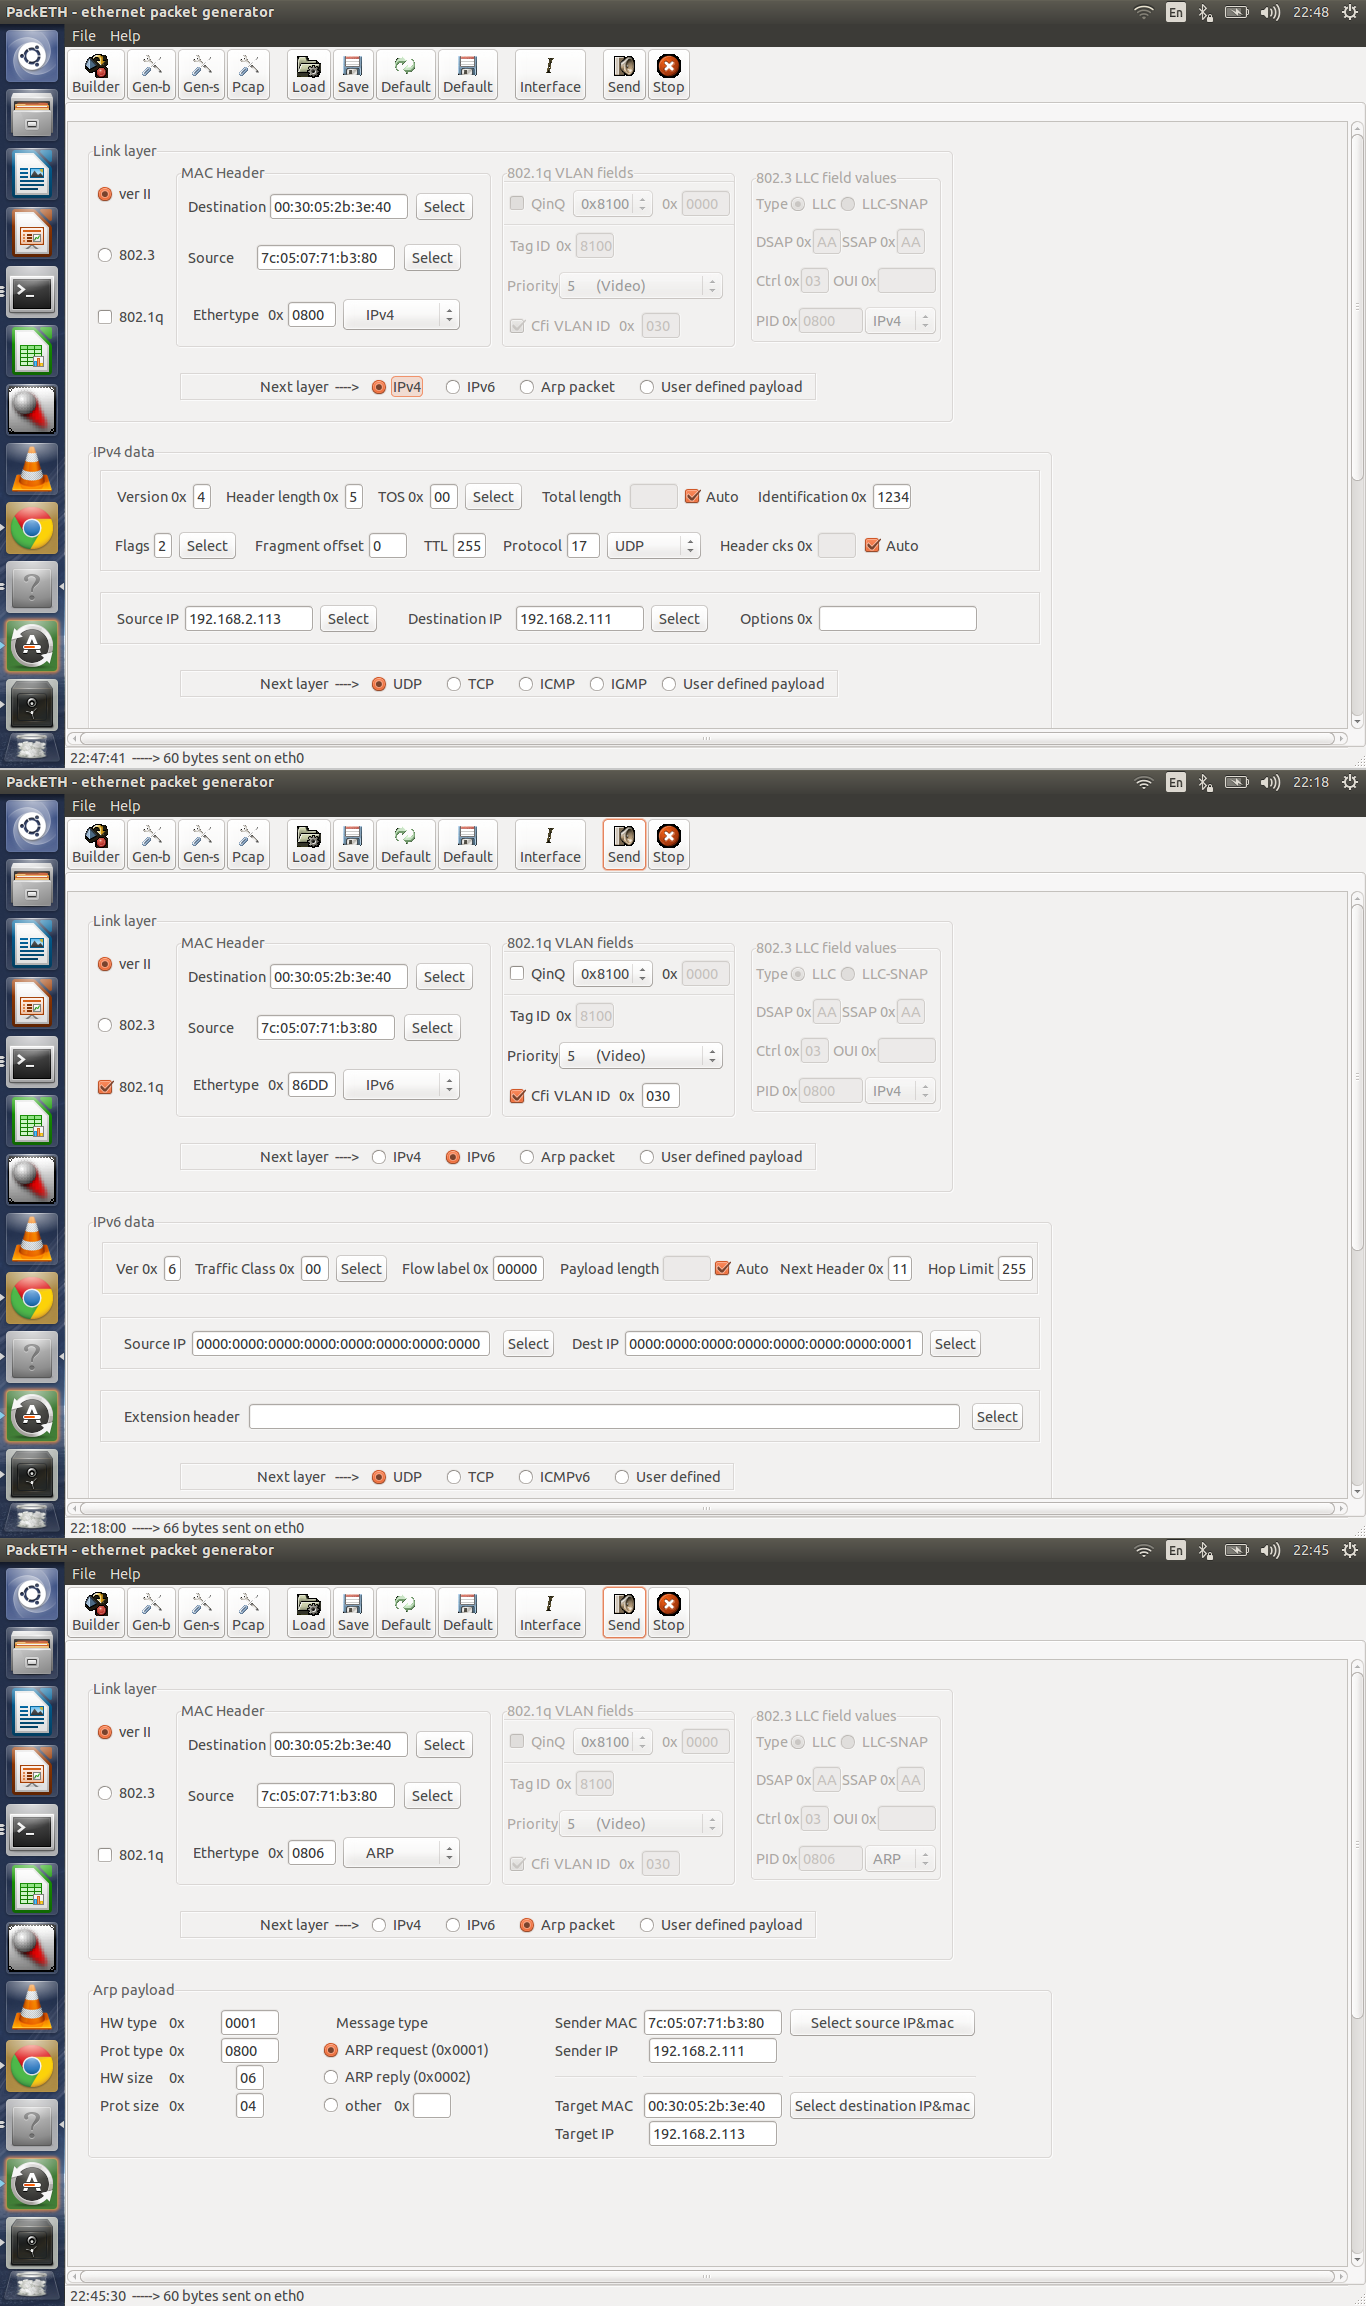
\includegraphics[width=0.50\textwidth]{Img1}
\caption[Jumper J16]{Jumper J16, Imagen extra\'ida de \citep{NetFPGA6}}
\label{fig:Img1}
\end{figure}

\item Setear el switch SW9 en la posición PCIe. Asegurarse bien de que el switch esta completamente puesto en dicha posición (figura ~\ref{fig:Img2}).

\begin{figure}[htbp!] 
\centering    
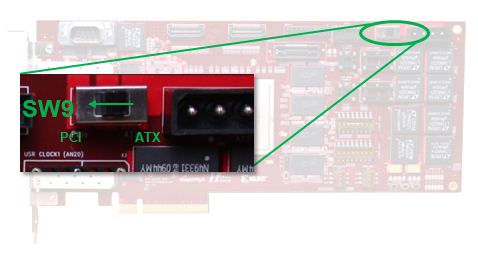
\includegraphics[width=0.50\textwidth]{Img2}
\caption[SW9 en posicion PCIe]{SW9 en posicion PCIe, Imagen extra\'ida de \citep{NetFPGA6}}
\label{fig:Img2}
\end{figure}

\item Asegurarse que los switches DIP SW1, SW2, SW6 y SW10 están correctamente ubicados acorde al siguiente esquema (figura ~\ref{fig:Img3}):\\

\textbf{SW1:} SEL0, SEL1, M2, M1, M0, N2, N1, N0 son seteados en off, off, off, on, on, on, off, off\\
\textbf{SW6:} SEL0, SEL1, M2, M1, M0, N2, N1, N0 son seteados en off, off, off, on, off on, off, on\\
\textbf{SW3:} M0, M1, M2 son seteados en on, on, on\\
\textbf{SW10:} SEL0, SEL1, SEL2 son seteados en on, off, off\\

\begin{figure}[htbp!] 
\centering    
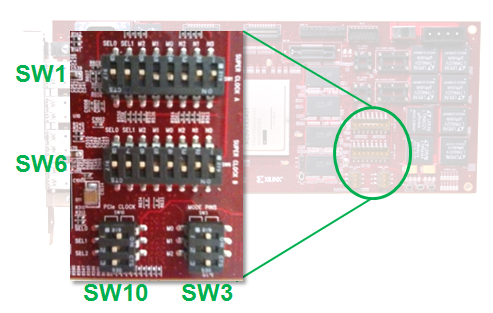
\includegraphics[width=0.50\textwidth]{Img3}
\caption[Posiciones DIP SW1 SW2 SW6 SW10]{Posiciones DIP SW1 SW2 SW6 SW10, Imagen extra\'ida de \citep{NetFPGA6}}
\label{fig:Img3}
\end{figure}

\item Con la PC apagada y desconectada de la electricidad instalar la tarjeta NetFPGA-10G en un slot PCIe disponible.

\item Conectar alguno de los conectores ATX disponibles de la PC al conector ATX de la tarjeta NetFPGA-10G (figura ~\ref{fig:Img4}).

\begin{figure}[htbp!] 
\centering    
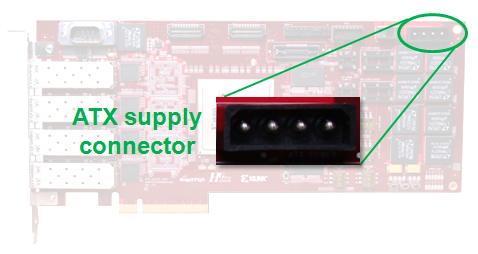
\includegraphics[width=0.50\textwidth]{Img4}
\caption[Conector ATX]{Conector ATX, , Imagen extra\'ida de \citep{NetFPGA6}}
\label{fig:Img4}
\end{figure}

\item Conectar el cable Samtec Twinax a la interfaz de expansión de la tarjeta formando un “loop” ( figura ~\ref{fig:Img5})

\newpage
\begin{figure}[htbp!] 
\centering    
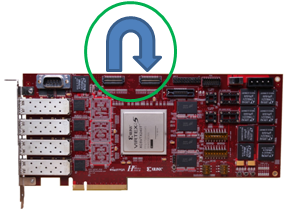
\includegraphics[width=0.40\textwidth]{Img5}
\caption[Cable samtec twinax]{Cable samtec twinax, , Imagen extra\'ida de \citep{NetFPGA6}}
\label{fig:Img5}
\end{figure}

\item Conectar un par de cables 10GE SFP+ a las interfaces de la tarjeta. Cada cable conecta dos puertos adyacentes formando dos “bucles” (ver figura ~\ref{fig:Img6}):

\begin{figure}[htbp!] 
\centering    
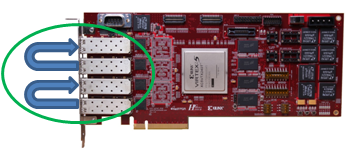
\includegraphics[width=0.50\textwidth]{Img6}
\caption[Cables samtec twinax conectados]{Cables samtec twinax conectados}
\label{fig:Img6}
\end{figure}

\item Conectar un cable serial RS232 al puerto serial RS232 en la tarjeta. Conectar el otro extremo en el puerto serial COM de la PC o a un adaptador USB por ejemplo (ver figura ~\ref{fig:Img7}).

\begin{figure}[htbp!] 
\centering    
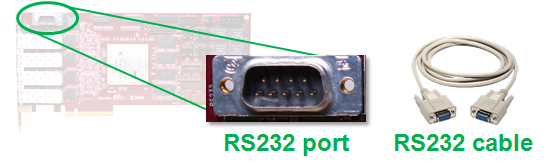
\includegraphics[width=0.50\textwidth]{Img7}
\caption[Cable serial puerto COM]{Cable seria puerto COM, Imagen extra\'ida de \citep{NetFPGA6}}
\label{fig:Img7}
\end{figure}

\item Conectar el cable de programación Xilinx JTAG al conector JTAG en la tarjeta. Luego conectar el otro extremo a la PC a través de un puerto USB por ejemplo (figura ~\ref{fig:Img8}).

\newpage
\begin{figure}[htbp!] 
\centering    
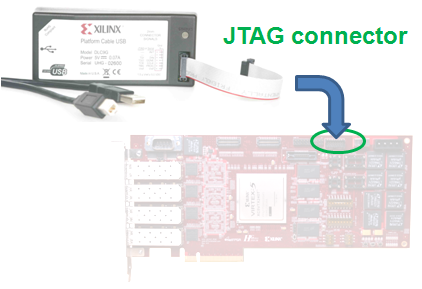
\includegraphics[width=0.55\textwidth]{Img8}
\caption[Cable JTAG]{Cable JTAG, Imagen extra\'ida de \citep{NetFPGA6}}
\label{fig:Img8}
\end{figure}

\end{itemize}

Al finalizar, la tarjeta NetFPGA debería estar instalada como se muestra en la siguientes figuras~\ref{fig:Img9}~\ref{fig:Img10}:

\begin{figure}[htbp!] 
\centering    
\includegraphics[width=0.80\textwidth]{Img9}
\caption[Tarjeta NetFPGA esquema de instalación]{Tarjeta NetFPGA esquema de instalación, Imagen extra\'ida de \citep{NetFPGA6}}
\label{fig:Img9}
\end{figure}

\newpage
\begin{figure}[htbp!] 
\centering    
\includegraphics[width=0.85\textwidth]{Img10}
\caption[Tarjeta NetFPGA instalada en una PC]{Tarjeta NetFPGA instalada en una PC}
\label{fig:Img10}
\end{figure}

Para ejecutar el Test de Producción seguir los siguientes pasos:

\begin{itemize}
\item Encender el PC y como usuario root abrir el archivo /boot/grub/grub.cfg con un editor de texto. Realizar las siguientes modificaciones:

\begin{itemize}
\item Localizar la entrada particular para la distribución del kernel que se tenga
\item Encontrar la línea que comienza con Kernel
\item Concatenar \textbf{memmap=256M\textbackslash\$0x5f700000} al final de la línea (ver figura ~\ref{fig:Img11}).\\
El parámetro memmap=256M\textbackslash\$0x5f700000 es pasado al kernel al momento de iniciar el sistema. El mismo reserva una región de 256MB de memoria disponible comenzando en la dirección 0x5f700000. Este bloque es utilizado posteriormente en el Test PCIe DMA.
\item Guardar los cambios realizados al archivo

\newpage
\begin{figure}[htbp!] 
\centering    
\includegraphics[width=0.95\textwidth]{Img11}
\caption[Reserva de bloque de memoria]{Reserva de bloque de memoria}
\label{fig:Img11}
\end{figure}

\end{itemize}

\item Iniciar la aplicación IMPACT de Xilinx indicando la opción “Yes” cuando se pregunte si queremos que la herramienta cree y guarde automáticamente un proyecto por nosotros.

\item Programar la CPLD con el diseño localizado en el directorio (ver figura ~\ref{fig:Img12})\\ 
/NF\_ROOT/projects/production\_test/bitfiles/cpld.jed

\begin{figure}[htbp!] 
\centering    
\includegraphics[width=0.45\textwidth]{Img12}
\caption[Programación Impact]{Programación Impact}
\label{fig:Img12}
\end{figure}

\item Programar la FPGA con el bitstream localizado en el directorio\\
/NF\_ROOT/projects/production\_test/bitfiles/prod\_test\_no\_rldram.bit

IMPACT posiblemente nos pregunte si queremos asociar un dispositivo PROM, seleccionar qué no. Programar la tarjeta puede llevar algún tiempo; de 10 a 20 minutos dependiendo del proyecto. Este proyecto en particular no debería tomar más de 10 minutos.

\item Reiniciar la PC

\item Verificar que el bloque de memoria DMA ha sido reservado correctamente a través de los siguientes pasos:

\begin{itemize}
\item Ejecutar en una consola:
\begin{bash}    
# cat /proc/cmdline
\end{bash}    
  
\item La salida debería ser similar a la figura ~\ref{fig:Img13}

\begin{figure}[htbp!] 
\centering    
\includegraphics[width=0.85\textwidth]{Img13}
\caption[Reserva bloque de memoria]{Reserva bloque de memoria}
\label{fig:Img13}
\end{figure}

\end{itemize}

\item Verificar que la tarjeta ha sido correctamente instalada siguiendo los siguientes pasos:

\begin{itemize}
\item Desde una consola verificar el dispositivo NetFPGA-10G ejecutando:
\begin{bash}
#lspci | grep Xilinx
\end{bash}

\item La salida debería ser similar a:
\begin{bash}
# 01:00.0 Ethernet controller: Xilinx Corporation Device 4244
\end{bash}

\end{itemize}

\item Desde la PC ejecutar el test de producción a través de los siguientes pasos:

\begin{itemize}
\item Situarse en la carpeta del Test de Producción
\begin{bash}
# cd projects/production_test/sw/
\end{bash}

\item Compilar el test
\begin{bash}
# make
\end{bash}

\item Posicionarse en la carpeta de scripts
\begin{bash}
# cd scripts
\end{bash}

\item Ejecutar el Test de Producción
\begin{bash}
# sudo ./production_test.py
\end{bash}

La salida debería ser como la que se muestra a continuación (ver figura ~\ref{fig:Img14}):

\newpage
\begin{figure}[htbp!] 
\centering    
\includegraphics[width=0.95\textwidth]{Img14}
\caption[Test de Producción salida esperada]{Test de Producción salida esperada}
\label{fig:Img14}
\end{figure}
\end{itemize}

\end{itemize}

Para ejecutar el RLDRAM Test recomendamos utilizar la guía \citep{NetFPGA8}.

\subsection{Programación de la tarjeta}

A continuación se describen los pasos necesarios para programar las tarjetas NetFPGA en particular con el proyecto ReferenceNIC. En lo que prosigue se utiliza NF\_ROOT para referirse al directorio donde se encuentra descargado el código fuente de NetFPGA.

\subsubsection{Configuración de la tarjeta}
Antes de comenzar, es necesario realizar algunas modificaciones en el hardware NetFPGA para habilitar la programación pcie del mismo, utilizada en la programación persistente.\\ 

Para habilitar la programación PCIe, es necesario cambiar la posición del switch Disp SW3 desde la posición por defecto (M0:On, M1:On, M2:On) a la posición de programación PCIE (M0:Off, M1:On, M2:On). Esta configuración habilita tanto la programación de la tarjeta por el cable de programación JTAG como por la interfaz PCIe.\\

La siguiente figura muestra la posición del Dip SW3 en la configuración PCIe (ver figura ~\ref{fig:Img15}).

\begin{figure}[htbp!] 
\centering    
\includegraphics[width=0.95\textwidth]{Img15}
\caption[Configuración SW3 JTag/PCIe programing]{Configuración SW3 JTag/PCIe programing}
\label{fig:Img15}
\end{figure}

Recordar que los cambios a la configuración de la tarjeta se deben realizar con la PC apagada y sin conexión a la corriente eléctrica para evitar daños en el hardware.\\

Una vez configurada la tarjeta conectar la PC a la corriente eléctrica y encender la misma.

\subsubsection{Programación de la tarjeta}
Antes que nada es necesario realizar algunos cambios en archivos del código fuente asociados a los proyectos NetFPGA utilizados, arreglando algunos errores reportados para la version de código fuente utilizada en este manual. Entonces en caso de trabajar con la versión 5.0.5 (recomendada) se deben realizar las siguientes modificaciones:

\begin{enumerate}

\item En el directorio NF\_ROOT/projects/reference\_nic/hw/ cambiar en el archivo \textit{system.mhs} lo siguiente:

\begin{bash}
PORT axi_emc_0_Mem_DQ_pin = axi_emc_0_Mem_DQ, DIR = IO, 
VEC = [*7*:0]
\end{bash}

cambiar por

\begin{bash}
PORT axi_emc_0_Mem_DQ_pin = axi_emc_0_Mem_DQ, DIR = IO, 
VEC = [*31*:0]
\end{bash}

\item En el directorio NF\_ROOT/projects/reference\_nic/hw/nf10 cambiar en el archivo \textit{xflow.opt} lo siguiente: 

\begin{bash}
-t *1*
\end{bash}

cambiar por

\begin{bash}
-t *5*
\end{bash}

(*) Los “*” no van

\item Modificar el driver utilizado por el proyecto ReferenceNIC:
\begin{enumerate}
\item Posicionarse en el directorio NF\_ROOT/projects/reference\_nic/sw/host/driver
\item Abrir el archivo nf10\_phy\_conf.c y comentar las líneas 217,219 y 240
\end{enumerate}

\end{enumerate}

Finalmente se debe compilar el proyecto. Para ello en una consola ejecutamos

\begin{bash}
# cd NetFPGA_ROOT/projects/reference_nic
# make
# cd cpld
# make
\end{bash}

Este proceso puede llevar de 10 a 20 minutos.\\

Ahora programamos la tarjeta NetFPGA con el proyecto ReferenceNIC, para lo cual es necesario conectar el cable de programación JTAG a la tarjeta y a la PC.\\

Luego en una consola se ejecuta lo siguiente:

\begin{bash}
# cd NetFPGA_ROOT
# cd tools/scripts
# ./impact_run 
  ../../projects/reference_nic/bit/reference_nic.bit 
  ../../projects/reference_nic/cpld/cpld.jed 
\end{bash}

(*) En caso de que aparezca el error “NF\_ROOT or NF\_DESIGN\_DIR variable is not defined”
abrir el script impact\_run.sh y definir una variable de nombre NF\_ROOT con el valor del directorio donde esta instalado el código fuente de NetFPGA.\\

Luego de finalizada la ejecución del comando reiniciar la máquina. Es sumamente importante que se reinicie y no que se apague, puesto que hasta el momento solo se ha programado el hardware en forma volátil. Esto quiere decir que de producirse un corte de corriente el misma se desprogramaría.\\

Una vez reiniciada la PC es necesario cargar el driver del ReferenceNIC en el kernel del sistema. Para ello posiblemente primero se deba compilar el driver. Para compilar el driver ejecutar en una consola:\\

\begin{bash}
# cd NetFPGA_ROOT/projects/reference_nic/sw/host/driver
# make
# insmod nf10.ko
\end{bash}

Ahora vamos a programar una de las memorias flash de la tarjeta (en particular utilizaremos la unidad A con el proyecto ReferenceNIC, de forma de hacer persistente la programación de la tarjeta.

Para ello en una consola ejecutamos:

\begin{bash}
# cd NF_ROOT/projects/reference_nic/bitfiles
# ./bit2bin.sh reference_nic.bit
\end{bash}

Con lo anterior se genera un archivo binario a partir del bitfile del proyecto, con el que programaremos la memoria. Luego de este comando se deberían de haber creado 3 archivos

\begin{itemize}
\item reference\_nic.prm
\item reference\_nic.bin
\item reference\_nic.cfi
\end{itemize}

Luego ejecutamos lo siguiente:

\begin{bash}
# cd ../sw/host/pcieprog
# ./nf10_configure -b ../../../bitfiles/reference_nic.bin -f a
\end{bash}

Apagamos la PC y la volvemos a prender. Ahora el chip FPGA de la tarjeta se encuentra programado a partir del contenido de la memoria flash A, con el proyecto que allí grabamos.\\

Para no cargar el driver del ReferenceNIC cada vez que se reinicie la máquina podemos modificar el archivo /etc/rc.local agregando la siguiente línea:

\begin{bash}
insmod NF_ROOT/preojects/reference_nic/sw/host/driver/nf10.ko
\end{bash}

\subsection{Instalación de Open vSwitch}
Open vSwitch (ovs) lo instalaremos también desde su código fuente ejecutando lo siguiente en una consola:

\begin{bash}
# wget http://openvswitch.org/releases/openvswitch-2.3.0.tar.gz
# tar zxvf openvswitch-2.3.0.tar.gz
# cd openvswitch-2.3.0
#./boot.sh
#./configure --with-linux=/lib/modules/\$(uname -r)/build
\end{bash}

Luego se compila el código fuente:

\begin{bash}
# make && make install
\end{bash}

Se inserta en el kernel de linux el módulo de ovs:

\begin{bash}
# cd datapath/linux
# modprobe openvswitch
\end{bash}

Podemos verificar que el módulo se insertó correctamente de la siguiente forma:

\begin{bash}
# lsmod | grep openvswitch

openvswitch    57291      0  
gre         14236         1     openvswitch
\end{bash}

Luego creamos el siguiente directorio necesario para la configuración del ovs:

\begin{bash}
# mkdir -p /usr/local/etc/openvswitch
\end{bash}

Finalmente creamos la base de datos de configuración de ovs:

\begin{bash}
# ovsdb-tool create /usr/local/etc/openvswitch/conf.db 
vswitchd/vswitch.ovsschema
\end{bash}

Ya se esta en condiciones de levantar cualquiera de los demonios de ovs. En particular para iniciar ovs debemos indicar una serie de parámetros como la base de datos donde se encuentra la configuración, en caso de utilizar una conexión segura con el controlador los certificados SSL correspondiente entre otras cosas. Para ello es conveniente crear un script como el siguiente:

\begin{bash}
ovsdb-server /usr/local/etc/openvswitch/conf.db \
--remote=punix:/usr/local/var/run/openvswitch/db.sock \
--remote=db:Open_vSwitch,Open_vSwitch,manager_options \
--private-key=db:Open_vSwitch,SSL,private_key \
--certificate=db:Open_vSwitch,SSL,certificate \
--bootstrap-ca-cert=db:Open_vSwitch,SSL,ca_cert 
--pidfile --detach --log-file

ovs-vsctl --no-wait init
ovs-vswitchd --pidfile --detach
ovs-vsctl show

\end{bash}

Por simplicidad hemos comentado las líneas relacionadas a la parte de seguridad en la comunicación entre el ovs y el controlador.\\

Finalmente para automatizar la carga de los drivers de Open vSwitch al encender la PC, crear una carpeta de nombre ovs dentro del directorio /lib/modules/\$(uname -r)/kernel/drivers
como se muestra a continuación.

\begin{bash}
# mkdir /lib/modules/$(uname -r)/kernel/drivers/ovs
# cd /lib/modules/$(uname -r)/kernel/drivers/ovs    
\end{bash}

Posteriormente copiar los archivos de extensión .o y .ko dentro de la carpeta de instalaci\'on de ovs (llamemos le OVS\_ROOT) en el siguiente directorio \\ OVS\_ROOT/datapath/linux al directorio anteriormente creado.\\

Finalmente ejecutamos el siguiente comando para actualizar las listas de dependencias para cada módulo agregado.

\begin{bash}
# depmod
\end{bash}

\subsection{Instalación de software de ruteo Quagga}
El software de ruteo Quagga puede instalarse con un gestor de aplicaciones (apt-get) o desde su código fuente; en este tutorial utilizamos esta ultima opción. 

El código fuente podemos obtenerlo desde el sitio oficial de quagga:

\begin{center}
http://www.nongnu.org/quagga/
\end{center}
 
o desde el siguiente link:

\begin{center}
http://www.nongnu.org/quagga/docs/docs-info.html\#OSPFv2
\end{center}

Una vez descargado el código fuente descomprimimos el archivo \textit{quagga.public-master.zip} en el directorio deseado. En este caso utilizaremos el directorio /home/mina como venimos haciendo para el resto del software instalado. Luego abrimos una consola y ejecutamos los siguientes comandos para compilar el código fuente:

\begin{bash}
# ./configure
# make 
\end{bash}

\subsection{Instalaci\'on de agente SNMP}
Para la instalaci\'on del agente SNMP se utiliza el gestor de paquetes de Ubuntu \textbf{apt-get} (en otras plataformas se podr\'ia utilizar por ejemplo opkg o yum).

Por lo tanto para instalar el agente SNMP ejecutamos en una consola lo siguiente:

\begin{bash}
# apt-get install snmp snmpd
\end{bash}

%\subsection{Extra}



% *************************************** Index ********************************
\printthesisindex % If index is present

\end{document}
